\documentclass[12pt,titlepage]{book}
\usepackage[margin=0.9in]{geometry} 
\usepackage{amsmath,amsthm,amssymb,graphicx,mathtools,tikz,hyperref}
\usepackage{pgfplots}
\usepackage{xcolor}
\newcommand{\redp}[1]{\textcolor{red}{#1}}
\newcommand{\bluep}[1]{\textcolor{blue}{#1}}
\newcommand{\tealp}[1]{\textcolor{teal}{#1}}
\usepackage{tcolorbox}
\newtcolorbox{mybox}{colback=red!5!white,colframe=red!75!black,fonttitle=\bfseries,title=Box}
\newtcolorbox{qt}{colback=orange!5!white,colframe=orange!75!white}
\usetikzlibrary{patterns,hobby}
\numberwithin{equation}{section}
\usepackage{wrapfig}
\usepackage{indentfirst}
\usepackage{ragged2e}
\RaggedRightParindent = 24 pt
\setlength{\parskip}{0.8em}
\renewcommand{\baselinestretch}{1.5}
\usepackage[noline]{algorithm2e}
\SetAlFnt{\footnotesize}
\usepackage{graphicx}
\usepackage{titling}
\renewcommand\maketitlehooka{\null\mbox{}\vfill}
\renewcommand\maketitlehookd{\vfill\null}
\usepackage{tocloft}
\renewcommand\cftsecafterpnum{\vskip6pt}
\usepackage{makeidx}
\makeindex
\usepackage{mdframed}
\newenvironment{que}
    { \begin{mdframed}[backgroundcolor=green!20] \textbf{$\Delta$ Question} \\}
    {  \end{mdframed}}
\newenvironment{thm}
    { \begin{mdframed}[backgroundcolor=orange!20] \textbf{$\Delta$ Theorem} \\}
    {  \end{mdframed}}
\newenvironment{defi}
    { \begin{mdframed}[backgroundcolor=red!10] \textbf{$\Delta$ Definition} \\}
    {  \end{mdframed}}
\newenvironment{lemma}
    { \begin{mdframed}[backgroundcolor=gray!10] \textbf{$\cdot$ Lemma} \\}
    {  \end{mdframed}}
\newenvironment{example}
    { \begin{mdframed}[backgroundcolor=white!10] \textbf{$\cdot$ Example} \\}
    {  \end{mdframed}}
\usepackage{graphicx}
\usepackage{float}
\usepackage{longtable}
\usepackage{tikz}
\usepackage{esint}
\usepackage{CJKutf8}
\usepackage{oubraces}
\usepackage{cancel}

\title{Quantum Field Theory for Educated Dummies}
\author{Sizhe Liu\\University of Illinois at Urbana-Champaign }
\date{Version 1.0}

\pgfplotsset{compat=1.15}

\begin{document}

\maketitle

\chapter{Foundations}
\section{Natural Units and Dimensions}
Convenient systems of units start with arbitrary definitions for units of certain fundamental. quantities and derive the remaining units from laws of nature. To see how this works, assume we know three basic laws of nature and we want to devise a system of units from scratch. We will do this first for the cgs system and then for natural units.
The three lawas are:
\begin{qt}
\begin{itemize}
    \item The distance $L$ traveled by a photon is the speed of light multiplied by its time of travel. $L=c t$
    \item The energy of a massive particle is equal to its mass (at rest) $m$ times the speed of light squared. $E=mc^2$
    \item The energy of a photon is proportional to its frequency $f$. The constant of proportionality is Planck's constant $h . E=h f$ or re-expressed as $E=\hbar \omega$
\end{itemize}
\end{qt}
In natural units:\redp{the $c$ and $\hbar$ are dimensionless and equal to 1. The unit for energy is $MeV$}.

\section{Notation}
We shall use a notation defining \textbf{contravariant components $x^{\mu}$ of the $4 \mathrm{D}$ position vector} as $3 \mathrm{D}$ Cartesian coordinates $X_{i}$ plus $c t$ (see Appendix $\bar{A}$ if you are not comfortable with this), i.e.,
\begin{equation}
x^{\mu}=\left[\begin{array}{l}
{x^{0}} \\
{x^{1}} \\
{x^{2}} \\
{x^{3}}
\end{array}\right]=\left[\begin{array}{l}
{c t} \\
{X_{1}} \\
{X_{2}} \\
{X_{3}}
\end{array}\right]=\left[\begin{array}{l}
{c t, X_{i}}
\end{array}\right]^{T}
\end{equation}
From special relativity, we know the differential proper time passed on an object (with $c=1$ ) is
\begin{equation}
(d \tau)^{2}=(d t)^{2}-d X_{1} d X_{1}-d X_{2} d X_{2}-d X_{3} d X_{3}
\end{equation}
If we define \textbf{covariant components} of the 4D position vector as
\begin{equation}
x_{\mu}=\left[\begin{array}{l}
{x_{0}} \\
{x_{1}} \\
{x_{2}} \\
{x_{3}}
\end{array}\right]=\left[\begin{array}{c}
{t} \\
{-X_{1}} \\
{-X_{2}} \\
{-X_{3}}
\end{array}\right]=\left[t,-X_{i}\right]^{T}
\end{equation}
then
\begin{equation}
(d \tau)^{2}=d x^{0} d x_{0}+d x^{1} d x_{1}+d x^{2} d x_{2}+d x^{3} d x_{3}=d x^{\mu} d x_{\mu}
\end{equation}
Using metric tensor $g_{\mu\nu}$, we have the following relation:
\begin{equation}
x_{\mu}=g_{\mu \nu} x^{\nu}=\left[\begin{array}{cccc}
{1} & {0} & {0} & {0} \\
{0} & {-1} & {0} & {0} \\
{0} & {0} & {-1} & {0} \\
{0} & {0} & {0} & {-1}
\end{array}\right]\left[\begin{array}{c}
{x^{0}} \\
{x^{1}} \\
{x^{2}} \\
{x^{3}}
\end{array}\right]
\end{equation}
\redp{The inverse of $g_{\mu\nu}$, $g^{\mu\nu}$, has the exact same form.}Thus,
\begin{equation}
(d \tau)^{2}=g_{\mu v} d x^{\mu} d x^{v}=g^{\mu v} d x_{\mu} d x_{v}
\end{equation}
\begin{qt}
Partial derivative w.r.t. $x^{\mu}$ and $x_{\mu}$ are:
\begin{equation}
\partial_{\mu}=\frac{\partial}{\partial x^{\mu}}=\left(\frac{\partial}{\partial t}, \frac{\partial}{\partial x^{i}}\right)^{T}=\left(\frac{\partial}{\partial t} \cdot \frac{\partial}{\partial X_{i}}\right)^{T}
\end{equation}
and
\begin{equation}
\partial^{\mu}=\frac{\partial}{\partial x_{\mu}}=\left(\frac{\partial}{\partial t}, \frac{\partial}{\partial x_{i}}\right)^{T}=\left(\frac{\partial}{\partial t},-\frac{\partial}{\partial X_{i}}\right)^{T}
\end{equation}
\end{qt}
For a matrix, we can raise the index as
\begin{equation}
M^{\mu \nu}=g^{\mu \alpha} g^{\nu \beta} M_{\alpha \beta}
\end{equation}
\section{Review of Variational Methods}
Recall also, that given the Lagrangian, we could find the Hamiltonian $H,$ via the Legendre transformation (employing a Cartesian system where $x^{i}=x_{i}$ and $p^{i}=p_{i}$),
\begin{equation}
H=p_{i} \dot{x}^{i}-L, \quad \text { where } p_{i}=\frac{\partial L}{\partial \dot{x}^{i}}=m \dot{x}^{i}\left(=p^{\prime} \text { for Cartesian system }\right)
\end{equation}
$p_{i}$ is the conjugate, or canonical, momentum of $x$ '. (Note that a contravariant component in the denominator is effectively equivalent to a covariant component in the entire entity, and vice versa.) Hence, we can define:
\begin{qt}
\textbf{First quantization}

Keeping the classical Hamiltonian and, changing Poisson brackets to commutators, we could just as readily have used the Lagrangian L, or the equations of motion instead.
\end{qt}
\subsection{Classical Field Theory}
From particle theory to field theory, we have the following things changed:
\begin{qt}
$$L, H, e t c \rightarrow \mathcal{L}, \mathcal{H},$$ 
\[
x^{i}(t) \rightarrow \phi^{r}\left(x^{\mu}\right)
\]
$$t \rightarrow x^{\mu}$$
\end{qt}
Classical field theory is analogous in many ways to classical particle Lagrangian $L$, we have the Lagrangian density $\mathcal{L}$. Instead of time $t$ as an independent variable, we have $x^{\mu}=x^{0}, x^{1}, x^{2}, x^{3}=t, {x^{i}}$ as independent variables. Instead of a particle described by $x^{i}(t),$ \textbf{we have a field value described by $\phi(x^{\mu})$, where $r$ designates different field types, or possibly, different spatial components of the same vector field.}
\begin{qt}
The Euler-Lagrange equation for fields becomes
\begin{equation}
\frac{\partial}{\partial x^{\mu}}\left(\frac{\partial \mathcal{L}}{\partial \phi^{r}, \mu}\right)-\frac{\partial \mathcal{L}}{\partial \phi^{r}}=0
\end{equation}
and
\begin{equation}
\mathcal{H}=\pi_{r} \dot{\phi}^{r}-\mathcal{L}, \quad \text { where } \pi_{r}=\frac{\partial \mathcal{L}}{\partial \dot{\phi}^{r}}
\end{equation}
with $\pi_r$ being the conjugate momentum density of the field $\phi^r$. And the action is
\begin{equation}
S=\int_{T} \int_{V} \mathcal{L}\left(\phi, \phi_{,\mu}\right) d^{3} \mathbf{x} d t=\int_{\Omega} \mathcal{L}\left(\phi, \phi_{, \mu}\right) d^{4} x
\end{equation}
\end{qt}
\subsection{Key concepts in field theory}
For fields
\begin{equation}
\frac{\partial \phi}{\partial t}=\frac{d \phi}{d t}=\dot{\phi}
\end{equation}
This is generally not true for other quantities. For fields, 
\begin{equation}
\frac{d \phi}{d t}=\frac{\partial \phi}{\partial x^{\prime}} \frac{d x^{\prime}}{d t}+\frac{\partial \phi}{\partial t} \frac{d t}{d t}
\end{equation}
\redp{where $\frac{dx^i}{dt}$ are equal to zero}.

For a single particle, particle position coordinates are the generalized coordinates and particle momentum components are its conjugate momenta. For fields, each field is itself a generalized coordinate and each field has its own conjugate momentum (density). As noted, this field conjugate momentum (density) is different from the physical momentum (density) that the field possesses.

For conjugate and physical momentum densities, we have the following density relation
$$
p_{t}=\frac{\partial L}{\partial \dot{x}^{t}} \quad \frac{\text { for small particle in medium, }}{\text { divide by particle volume }}, \quad \mathcal{R}_{i}=\frac{\partial \mathcal{L}}{\partial \dot{x}^{i}}
$$
We note carefully that our $x^i$ here is the position coordinate of a point fixed relative to the field and thus is time dependent. Further, the total derivative $\dot{x}^i$ equals the partial derivative w.r.t. time, since $x^i$ in the present case is only a function of time. Now take the \redp{conjugate momentum density relation for relativistic fields},
$$
\pi_{r}=\frac{\partial \mathcal{L}}{\partial \dot{\phi}^{r}}
$$
and
$$
\frac{\mathcal{R}_{i}}{\pi_{r}}=\frac{\partial \mathcal{L} / \partial \dot{x}^{i}}{\partial \mathcal{L} / \partial \dot{\phi}^{r}}=\frac{\partial \dot{\phi}^{r}}{\partial \dot{x}^{\prime}}=\frac{\partial \phi^{r} / \partial t}{\partial x^{i} / \partial t}=\frac{\partial \phi^{r}}{\partial x^{i}} \quad \rightarrow \quad \mathcal{R}_{i}=\pi_{r} \frac{\partial \phi^{r}}{\partial x^{i}} \quad \rightarrow \quad \mathcal{R}^{i}=-\pi_{r} \frac{\partial \phi^{r}}{\partial x^{i}}
$$
The partial derivative of $\phi^{r}$ with respect to either of our definitions of $x^{i}$ (time dependent as the moving position of a point fixed to the field, or time independent as coordinates fixed in space) is the same because by definition, partial derivative means we hold everything else here constant, Thus, the above relation holds in field theory when we consider the $x^{i}$ as independent variables (coordinates fixed in space).

The field equation (equations of motion) for relativistic fields keep the exact same form in any inertial frame of reference, i.e., they are \redp{Lorentz invariant}. Four scalars(world scalars) are \redp{invariant under a Lorentz transformation and look exactly the same to any observer.}
\begin{qt}
The mass $m$ in relativity of a free particle is four scalar, where $m^2=p^{\mu}p_{\mu}$.

Demanding that the Euler-Lagrange equation be Lorentz invariant, we know that, within that equation, $x^{\mu}$,$\phi^r$, and derivatives of $x^{\mu}$ are Lorentz covariant or invariant. \redp{So, in order for the whole equation to be Lorentz invariant, the Lagrangian density $\mathcal{L}$ must be invariant.}

Further, L, H, and $\mathcal{H}$ are not Lorentz scalars.
\end{qt}

\section{Schrodinger vs. Heisenberg Pictures}
In Schrodinger picture, the expectation value is calculated as:
$$
\overline{\mathcal{O}}=\int \psi^{\dagger} \mathcal{O} \psi d^{3} x=\langle\psi|\mathcal{O}| \psi\rangle
$$
The time derivative of the expectation value is
\begin{equation}
\frac{d \bar{\mathcal{O}}}{d t}=\frac{d}{d t}\langle\psi|\mathcal{O}| \psi\rangle=\left\langle\frac{\partial \psi}{\partial t}|\mathcal{O}| \psi\right\rangle+\left\langle\psi\left|\frac{\partial \mathcal{O}}{\partial t}\right| \psi\right\rangle+\left\langle\psi|\mathcal{O}| \frac{\partial \psi}{\partial t}\right\rangle
\end{equation}
where we use partial derivative in the brackets because our states and operators are functions of $x^i$ and $t$.

In the Schródinger picture (S.P.), the solutions to the Schrödinger equation

\begin{equation}
i \frac{\partial \psi_{S}}{\partial t}=H \psi_{S} \quad \text { or } \quad i \frac{\partial}{\partial t}|\psi\rangle_{S}=H|\psi\rangle_{S}
\label{schrodinger-equation}
\end{equation}
\redp{In the Schrodinger picture, the operators are usually not time dependent.} For example, using the familiar momentum operator $p_1^S=i\partial/\partial x^1$ for the S.P. in the $x^1$ direction, with 
$$
\psi_{S}=A e^{-i\left(E t-p\cdot x\right)}=|\psi\rangle_{S} \quad A^{\dagger} A=\frac{1}{V}
$$
we have
$$
\begin{array}{l}
{\bar{p}_{1}=\int A^{+} e^{i\left( Et-p^{\prime}x^{\prime}\right)}\left(i \frac{\partial}{\partial x^{1}}\right) A e^{-i\left(Et-p^{\prime}x^{\prime}\right)} d^{3} x={}_{s}\langle\psi|p_{1}^{S}| \psi\rangle_{s}}
\end{array}
$$
Since there is no $t$ in the operator, we have
$$
\frac{d p_{1}^{S}}{d t}=\frac{\partial p_{1}^{S}}{\partial t}=0
$$
and
\begin{equation}
\frac{d \bar{p}_{1}}{d t}=\frac{d}{d t}\left\langle\psi\left|p_{1}^{s}\right| \psi\right\rangle=\left\langle\frac{\partial \psi}{\partial t}\left|p_{1}^{s}\right| \psi\right\rangle_{s}+s\left\langle\psi\left|\frac{\partial p_{1}^{s}}{\partial t}\right| \psi\right\rangle_{s}+s\left\langle\psi\left|p_{1}^{s}\right| \frac{\partial \psi}{\partial t}\right\rangle_{s}
\end{equation}
Using (\ref{schrodinger-equation}), and its complex conjugate, we have
\begin{equation}
\frac{d \bar{p}_{1}}{d t}=_{S}\left\langle\psi\left|\left(i H p_{1}^{S}+\frac{\partial p_{1}^{S}}{\partial t}-i p_{1}^{S} H\right)\right| \psi\right\rangle_{S}=_{S}\left\langle\psi\left|-i\left[p_{1}^{S}, H\right]\right| \psi\right\rangle_{S}+_{S}\left\langle\psi\left|\frac{\partial p_{1}^{S}}{\partial t}\right| \psi\right\rangle_{S}
\end{equation}
where the last term is equal to zero.\redp{Recall the old NRQM adage that the expectation value of any operator without explicit time dependence that commutes with the Hamiltonian is conserved (its time derivative is zero.)}

\textbf{\redp{The Schrodinger picture states and operators can be transformed to states and operators having different form via what is known as a unitary transformation. The particular unitary transformation (where $U$ is a unitary operator) for this is}}
\begin{qt}
\begin{equation}
U=e^{-i A t} \quad\left(=e^{-i H t / \hbar} \text { in non-natural units }\right)
\end{equation}
where states and operators transform as
\begin{equation}
\begin{array}{ll}
{U^{\dagger}|\psi\rangle_{S}=|\psi\rangle_{H}} & {U^{\dagger} \mathcal{O}^{S} U=\mathcal{O}^{H}} \\
{U|\psi\rangle_{H}=|\psi\rangle_{S}} & {U O^{H} U^{\dagger}=\mathcal{O}^{S}}
\end{array}
\end{equation}
\end{qt}
We find that in the first relation the state is now \redp{time independent} in H.P. 

Taking the time derivative in the second relation, we have:
\begin{equation}
\begin{aligned}
\frac{d}{d t}\left(U^{\dagger} \mathcal{O}^{S} U\right) &=(i H) \underbrace{e^{i A^{\prime}} \mathcal{O}^{S}}_{\mathcal{O}^{H}}+\underbrace{e^{i H_{t}}\left(\frac{\partial \mathcal{O}^{S}}{\partial t}\right) e^{-i H_{l}}}_{\text {defined as } \hat{\partial} O^{H} / \partial t}+\underbrace{e^{i H t} \mathcal{O}^{S} e^{-t H t}}_{\mathcal{O}^{H}}(-i H) \\
&=\frac{d \mathcal{O}^{H}}{d t}=-i\left[\mathcal{O}^{H}, H\right]+\frac{\hat{\partial} \mathcal{O}^{H}}{\partial t}
\end{aligned}
\end{equation}
In this note, $\frac{\hat{\partial} \mathcal{O}^{H}}{\partial t}$ will always be zero. Nonetheless, we see that in the H.P., an operator time derivative can be \textbf{non-zero},\redp{and the operator is time dependent}.
\begin{mybox}
A unitary transformation is called unitary because its operation on (transformation of ) a state vector leaves the magnitude of the state vector unchanged, i.e., the state vector magnitude is multiplied by unity.

A unitary transformation can be thought of as "rotating" a (complex number) state vector in Hilbert space (the complex space where each coordinate axis is an eigenvector) without changing the "length".

Recall, from classical mechanics, that an orthogonal transformation represented by a real matrix $\mathbf{A}$ has an inverse equal to the transpose of that matrix, i.e., $\mathrm{A}^{-1}=\mathrm{A}^{\mathrm{T}}$. In the complex space of state vectors, a unitary transformation $U$ has an analogous form for its inverse, the complex conjugate transpose, i.e., $\underline{U}^{-1}=U^{+}$ and so $U^{\dagger} U=1 .$ The following example may make this clearer.

Do a Taylor expansion of $U=e^{-i H t}$ above about $t$, when $U$ is operating on an energy eigenstate., i.e.,
\begin{equation}
U\left|\psi_{E}\right\rangle= e^{-iHt}\left|\psi_{E}\right\rangle=\left(1-i t H-\frac{1}{2} t^{2} H^{2}+\ldots\right)\left|\psi_{E}\right\rangle= e^{-i E t}\left|\psi_{E}\right\rangle
\end{equation}
\end{mybox}
\textbf{Note:} Although it is common to write $U=e^{-iHt}$,\bluep{it is implied that $H$ (if you think of it as $i\partial/\partial t$) does not act on $t$. To be proper, the $t$ should be placed before the $H$, as we did in the expansion above, but it usually is not done that way.}

\redp{Because $H=H^S$ commutes with itself, $U$ and $U^+$ commute with $H$, so using $\mathcal{O}^S=H^S=H$, we have}
\begin{equation}
    H=H^S=H^H
\end{equation}
and after inserting $UU^+=1$, we find
\begin{equation}
\begin{aligned}
\frac{d \overline{\mathcal{O}}}{d t} &=s\left(\psi\left|U U^{\dagger}\left(-i\left[\mathcal{O}^{S}, H\right]\right) U U^{\dagger}\right| \psi\right\rangle_{s}+_{S}\left\langle\psi\left|U U^{+} \frac{\partial \mathcal{O}^{S}}{\partial t} U U^{\dagger}\right| \psi\right\rangle_{S} \\
&=_{H}\left\langle\psi\left|\left(-i\left[\mathcal{O}^{H}, H\right]\right)\right| \psi\right\rangle_{H}+{}_{H}\left\langle\psi\left|\frac{\hat{\partial} \mathcal{O}^{\mu}}{\partial t}\right| \psi\right\rangle_{H}
\end{aligned}
\end{equation}
\section{Extrapolation to Field Theory}
\textbf{According to the correspondence principle, in the macroscopic limit, our quantum relations must reduce to the usual classical relations.} So the principle provides us with a key part of our method for quantization. That is, in going from classical theory to NRQM, we must take
$$\left\{x^{\prime}, p_{j}\right\}=\delta_{j}^{i} \quad \substack{\longrightarrow\\ \text { 1st quantization }} \quad\left[x^{i}, p_{j}\right]=i \hbar \delta_{j}^{i}$$
For field theory, we have
\begin{qt}
\begin{equation}
\left\{\phi^{r}(\mathrm{x}, t), \pi,(\mathrm{y}, t)\right\}=\delta^{r}{ }_s \delta(\mathrm{x}-\mathrm{y})\substack{\longrightarrow\\ \text{2nd quantization}}\left[\phi^{r}, \pi_{s}\right]=i \hbar \delta^{r}{ }_s \delta(\mathbf{x}-\mathbf{y}) 
\end{equation}
and
\begin{equation}
    \left[\phi^{r}, \phi^{s}\right]=\left[\pi_{r}, \pi_{s}\right]=0
\end{equation}
\end{qt}
Again, \redp{Quantization is a means for deducing quantum theory from classical theory.}

\section{Appendix: some useful math relations}
First, we have four-velocity of relativity $u^{\mu}$ for an object as:
\begin{equation}
u^{\mu}=\frac{d x^{\mu}}{d \tau}=\frac{d}{d \tau}\left[\begin{array}{ccc}
{x^{0}} & {x^{1}} & {x^{2}}
\end{array}\right]=\left[\begin{array}{cccc}
{u^{0}} & {u^{1}} & {u^{2}} & {u^{3}}
\end{array}\right]
\end{equation}
where
\begin{equation}
u^{i}=\frac{d x^{i}}{d \tau}=\frac{d x^{i}}{\sqrt{1-v^{2} / c^{2}} d t}=\frac{v^{i}}{\sqrt{1-v^{2} / c^{2}}}=\gamma v^{i}
\end{equation}
\begin{equation}
u^{0}=\frac{d x^{0}}{d \tau}=c \frac{d t}{d \tau}=\frac{c}{\sqrt{1-v^{2} / c^{2}}}=\gamma c
\end{equation}
Thus,
\begin{equation}
(u)^{2}=\left|u^{\mu}\right|^{2}=\mu^{\mu} u_{\mu}=\frac{d x^{\mu}}{d \tau} \frac{d x_{\mu}}{d \tau}=\gamma^{2}\left(c^{2}-\left(v^{1}\right)^{2}-\left(v^{2}\right)^{2}-\left(v^{3}\right)^{2}\right)=c^{2}
\end{equation}

The magnitude of the \redp{4-momentum $p^{\mu}=mu^{\mu}$} is  then found from:
\begin{equation}
(p)^{2}=\left|p^{\mu}\right|^{2}=p^{\mu} p_{\mu}=m^{2} u^{\mu} u_{\mu}=m^{2} c^{2} \quad\left(=m^{2} \text { in natural units }\right)
\end{equation}
\bluep{Note that $p^0=\gamma mc=E/c$, where $E$ is relativistic energy, and $p^i$ is relativistic 3-momentum.} Or
\begin{equation}
    \begin{array}{l}
{p^{\mu} p_{\mu}=m^{2} c^{2}=g_{\mu \nu} p^{\mu} p^{\nu}=\left[\begin{array}{cccc}
{E / c} & {p^{1}} & {p^{2}} & {p^{3}}
\end{array}\right]\left[\begin{array}{c}
{E / c} \\
{-p^{1}} \\
{-p^{2}} \\
{-p^{3}}
\end{array}\right]}
\end{array}
\end{equation}

and
\begin{equation}
\frac{E^{2}}{c^{2}}=p^{2}+m^{2} c^{2}
\end{equation}
\chapter{Scalars: Spin 0 Fields}
\section{Deducing Klein-Gordon Equation}
If we squared the operators in the original Schrodinger equation, we obtain
\begin{equation}
\left(i \hbar \frac{\partial}{\partial t}\right)\left(i \hbar \frac{\partial}{\partial t}\right) \phi=H^{2} \phi=\left(\mathbf{p}_{o p e r}^{2} c^{2}+m^{2} c^{4}\right) \phi
\end{equation}
which becomes
\begin{equation}
-\frac{\hbar^{2}}{c^{2}} \frac{\partial^{2}}{\partial t^{2}} \phi=\left(-\hbar^{2} \frac{\partial}{\partial X_{i}} \frac{\partial}{\partial X_{i}}+m^{2} c^{2}\right) \phi
\end{equation}
In a compact form, we have
\begin{equation}
-\frac{\partial}{\partial x^{0}} \frac{\partial}{\partial x_{0}} \phi=\left(\frac{\partial}{\partial x^{i}} \frac{\partial}{\partial x_{i}}+\frac{m^{2} c^{2}}{\hbar^{2}}\right) \phi
\end{equation}
where we define $\mu^2=\frac{m^{2} c^{2}}{\hbar^{2}}$. Re-arranging, we have the Klein-Gordon equation
\begin{qt}
    \begin{equation}
\left(\partial_{\mu} \partial^{\mu}+\mu^{2}\right) \phi=0
\end{equation}
The operation $\partial_{\mu} \partial^{\mu}=\partial^{\mu} \partial_{\mu}$ is called the \textbf{d'Alembertian} operator, and is the 4D Minkowski coordinates analogue of the 3D Laplacian operator of Cartesian coordinates.
\end{qt}
\subsection{The solutions to the Klein-Gordon Equation}
\begin{equation}
\phi(x)=\sum_{n=1}^{\infty} \frac{1}{\sqrt{2 V E_{n} / \hbar}}\left(A_{n} e^{-\frac{i}{\hbar}\left(E_{n} t-\mathbf{p}_{n} \cdot \mathbf{x}\right)}+\underbrace{B_{n}^{\dagger} e^{\frac{i}{\hbar}\left(E_{n} t-\mathbf{p}_{n} \cdot \mathbf{x}\right)}}_{\text {absent in NRQM }}\right)
\end{equation}
Because we are using the square of the relativistic Hamiltonian in RQM, \bluep{we get additional solutions of exponential form $+i(E_nt-\mathbf{p}_n\cdot\mathcal{x})/\hbar$ that also solve the relativistic Klein-Gordon equation}.

With an aim towards using natural units, we note the following relations, where wave number $k_{i}$ $=2 \pi / \lambda_{i}$ and we use the deBroglie relation $p^{i}=\hbar k^{i}$
\begin{qt}
    \begin{equation}
p_{\mu}=\left[\begin{array}{c}
{E / c} \\
{p_{i}}
\end{array}\right]=\left[\begin{array}{c}
{E / c} \\
{-p^{i}}
\end{array}\right]=\hbar k_{\mu}=\left[\begin{array}{c}
{\hbar \omega / c} \\
{-\hbar k^{\prime}}
\end{array}\right]
\end{equation}
in natural units
\begin{equation}
p_{\mu}=\left[\begin{array}{c}
{E} \\
{-p^{i}}
\end{array}\right]=k_{\mu}=\left[\begin{array}{c}
{\omega} \\
{-k^{i}}
\end{array}\right]
\end{equation}
\end{qt}
Recall the notation introduced in the previous chapter, we have
\begin{equation}
p x=p_{\mu} x^{\mu}=E t-p^{i} x^{i}=p^{\mu} x_{\mu}
\end{equation}
\begin{equation}
k x=k_{\mu} x^{\mu}=\omega t-k^{i} x^{i}=\frac{E t}{\hbar}-\frac{p^{i} x^{i}}{\hbar}=\frac{p_{\mu}}{\hbar} x^{\mu}
\end{equation}
In natural unit
\begin{equation}
E=\omega, \quad p_{i}=k_{i}, \quad p_{\mu}=k_{\mu}, \quad p x=k x
\end{equation}
\bluep{For free fields, a given wave with wave number vector $\mathbf{k}$ has a particular energy, and we can designate that energy via either $E_{\mathbf{k}} \text { or } \omega_{\mathbf{k}} .$ It is common practice for scalars to use $\mathbf{k} \text { (rather than } \mathbf{p})$ and $\mathbf{k}$ (rather than $E_{\mathbf{p}}$ or $E_{\mathbf{k}}$.)}

The Klein-Gordon equation solutions then become, in natural units
\begin{equation}
\phi(x)=\sum_{k} \frac{1}{\sqrt{2 V_{e l}}}\left(A_{k} e^{-i k x}+B_{k}^{\dagger} e^{i k x}\right)
\end{equation}
\begin{mybox}
In RQM, the solution $\phi$ is that of a general (sum of eigenstates) single particle state. Each eigenstate has mathematical form of
$$
\phi_{k, A}=\frac{e^{-i k x}}{\sqrt{V}}
$$
$$
\quad \phi_{\mathrm{k}, B^{\dagger}}=\frac{e^{i k x}}{\sqrt{V}}
$$
Each of these forms has what is called \textbf{unit norm}. That is, all such eigenstates are \textbf{orthonormal}:
\begin{equation}
\int \phi_{k, A}^{\dagger} \phi_{k^{\prime},A} d^{3} x=\frac{1}{V} \int e^{i k x} e^{-i k^{\prime} x} d^{3} x=\delta_{k k^{\prime}}
\end{equation}
Similar relations exist for $\phi_{k, B^{\dagger}}$.
\end{mybox}

\subsection{Deducing probability density in RQM}
Starting from the Klein-Gordon equation, first post-multiply it by $\phi^{\dagger}$, then subtract the complex conjugate equation post-multiplied by $\phi$,
\begin{equation}
\begin{array}{c}
{\left\{\frac{\partial^{2}}{\partial t^{2}} \phi=\left(\nabla^{2}-\mu^{2}\right) \phi\right\} \phi^{\dagger}} \\
{-\left\{\frac{\partial^{2}}{\partial t^{2}} \phi^{\dagger}=\left(\nabla^{2}-\mu^{2}\right) \phi^{\dagger}\right\} \phi}
\end{array}
\end{equation}
Since $\mu^{2} \phi^{\dagger} \phi-\mu^{2} \phi \phi^{\dagger}=0$, we obtain
\begin{equation}
i \frac{\partial}{\partial t}\left(\frac{\partial \phi}{\partial t} \phi^{\dagger}-\frac{\partial \phi^{\dagger}}{\partial t} \phi\right)=i \nabla \cdot\left((\nabla \phi) \phi^{\dagger}-\left(\nabla \phi^{\dagger}\right) \phi\right)
\end{equation}
where probability density and the probability current for a Klein-Gordon particle are
\begin{qt}
    \begin{equation}
\rho=j^{0}=i\left(\frac{\partial \phi}{\partial t} \phi^{\dagger}-\frac{\partial \phi^{\dagger}}{\partial t} \phi\right)
\end{equation}
and
\begin{equation}
\mathbf{j}=-i\left((\nabla \phi) \phi^{\dagger}-\left(\nabla \phi^{\dagger}\right) \phi\right) \quad j^{i}=-i\left(\phi_{,i} \phi^{\dagger}-\phi_{, i}^{\dagger} \phi\right)=i\left(\phi^{,i} \phi^{\dagger}-\phi^{\dagger, i} \phi\right)
\end{equation}
\end{qt}
Now we can define the \redp{4-currents} as
\begin{equation}
j^{\mu}=\left[\begin{array}{l}
{\rho} \\
{\mathbf{j}}
\end{array}\right]=\left[\begin{array}{l}
{\rho} \\
{j^{i}}
\end{array}\right]=\left[\begin{array}{l}
{j^{0}} \\
{j^{i}}
\end{array}\right]=i\left(\phi^{\mu} \phi^{\dagger}-\phi^{\dagger,\mu} \phi\right)
\end{equation}
The \redp{4D continuity equation} is then
\begin{qt}
    \begin{equation}
\frac{\partial j^{\mu}}{\partial x^{\mu}}=\partial_{\mu} j^{\mu}=j^{\mu}{ }_{,\mu}=0
\label{4d-continuity-eq}
\end{equation}
\end{qt}
(\ref{4d-continuity-eq}) tells us the important fact that \bluep{the 4-divergence of the 4-current of any conserved quantity is zero}.

\bluep{The total probability of unity is a relativistic invariant. Further $A_{k}$ here are constants that do not vary with frame.}\redp{So the probability of  finding any particular state is also independent of what frame the measurements are taken in.}

\subsection{Negative Energies in RQM}
If we apply traditional Hamiltonian operator $H$ as $i\partial/\partial t$ to $\phi_{\mathbf{k},B^{\dagger}}$:
\begin{equation}
i \frac{\partial \phi_{\mathbf{k}, B^{\dagger}}}{\partial t}=i \frac{\partial}{\partial t} \frac{e^{i k x}}{\sqrt{V}}=-\omega_{\mathbf{k}} \frac{e^{i k x}}{\sqrt{V}}=-\omega_{\mathbf{k}} \phi_{\mathbf{k}, B^{\dagger}}=E_{\mathbf{k}, B^{\prime}} \phi_{\mathbf{k}, B^{+}}
\end{equation}
Since $\omega_{\mathbf{k}}$ is always a positive number, we have states with \redp{negative energies in RQM, and we need QFT to solve this dilemma}. 

\section{Klein-Gordon Equation in Quantum Field Theory}

\chapter{Spinors: Spin 1/2 Fields}
\section{Dirac's Approach to RQM:}
Dirac's primary goal was a 1st order relativistic Schrodinger equation, and he postulated that if it existed, it must have the general form of 
\begin{equation}
i \frac{\partial}{\partial t}|\psi\rangle= H|\psi\rangle=(a \cdot \mathbf{p}+\beta m)|\psi\rangle
\label{1st-order-relativistic-SDE}
\end{equation}
In \ref{1st-order-relativistic-SDE}, $\mathbf{p}$ is particle three momentum (an operator in quantum theories), and the vector $\alpha$ and the scalar $\beta$ would have to be determined. Thus, the equation would be first order in the time derivative. To find $\alpha$ and $\beta$, Dirac reasoned that $H^{2}$ and $|\psi\rangle$ must also satisfy the usual relativistic energy momentum relation (and therefore the Klein-Gordon equation)
$$
-\frac{\partial^{2}}{\partial t^{2}}|\psi\rangle= H^{2}|\psi\rangle=\left(\mathbf{p}^{2}+m^{2}\right)|\psi\rangle
$$
Thus
$$
-\frac{\partial^{2}}{\partial t^{2}}|\psi\rangle= H^{2}|\psi\rangle=\left(\alpha_{i} p_{i}+\beta m\right)\left(\alpha_{j} p_{j}+\beta m\right)|\psi\rangle
$$
$$
=\left(\alpha_{i}^{2} p_{i}^{2}+\underbrace{\left(\alpha_{i} \alpha_{j}+\alpha_{j} \alpha_{i}\right)}_{\text {must }=0}p_{i}p_{j}+\underbrace{\left(\alpha_{i} \beta+\beta \alpha_{i}\right)}_{\text {must }=0} p_{i} m+\beta^{2} m^{2}\right)|\psi\rangle
$$
Therefore, $\alpha_{i}^{2}=1$ and $\beta^{2}=1$. In summary, we have anti-commutators relationship:
\begin{qt}
    \begin{equation}
\begin{aligned}
&\left[\alpha_{i}, \alpha_{j}\right]_{+}=\left[\alpha_{i}, \beta\right]_{+}=0 \quad i \neq j \quad \alpha_{1}, \alpha_{2}, \alpha_{3}, \beta \text { all anti-commute with each other, }\\
&\left(\alpha_{1}\right)^{2}=\left(\alpha_{2}\right)^{2}=\left(\alpha_{3}\right)^{2}=(\beta)^{2}=1 \text { (the identity matrix) }
\end{aligned}
\label{standard-condition}
\end{equation}
\end{qt}
\bluep{If $\alpha_{i}$ and $\beta$ were numbers they would have to commute and could not possibly anti-commute. Hence, they can only be matrices. since these matrices are operators operating on $|\psi\rangle,$ then $|\psi\rangle$ itself must be a multicomponent object (i.e., a column matrix, at least.)}. Use the relations above, one can show that the \redp{$\alpha$ and $\beta$ matrices are traceless, hermitian, have $\pm$ eigenvalues, and must have an even dimension of at least four}.

Square matrices in a 4D space must be  $4\mathrm{X} 4,$ and thus if $|\psi\rangle$ is a column matrix (a vector), it must have four components (a 4D vector). Take care to note the \bluep{4D space we are talking about here is not the four-dimensional physical space of relativity theory, but an abstract pace, often called \textbf{spinor space}}.
\subsection{Standard presentation}
Choosing the minimum dimension case (four), Dirac and Pauli came up with a set of matrices which solve all of the conditions in (\ref{standard-condition}):
$$
\beta=\left[\begin{array}{cccc}
{1} \\
{} & {1} \\
{} & {} & {-1} \\
{} & {} & {} & {-1}
\end{array}\right]
$$
$$
\alpha_{1}=\left[\begin{array}{cccc}
{}&{}&{}&{1} \\
{}&{}&{1} \\
{} & {1} \\
{1}
\end{array}\right] \quad \alpha_{2}=\left[\begin{array}{cccc}
{}&{}&{}&{-i} \\
{}&{}&{i} \\
{} & {-i} \\
{i}
\end{array}\right] \quad \alpha_{3}=\left[\begin{array}{cccc}
{}&{}&{1} \\
{}&{}&{}& {-1} \\
{1}\\
{}&{-1} 
\end{array}\right]
$$
which are commonly written using Pauli matrices
$$
\beta=\left[\begin{array}{cc}
{I} & {0} \\
{0} & {-I}
\end{array}\right] \quad \alpha_{1}=\left[\begin{array}{cc}
{0} & {\sigma_{1}} \\
{\sigma_{1}} & {0}
\end{array}\right] \quad \alpha_{2}=\left[\begin{array}{cc}
{0} & {\sigma_{2}} \\
{\sigma_{2}} & {0}
\end{array}\right] \quad \alpha_{3}=\left[\begin{array}{cc}
{0} & {\sigma_{3}} \\
{\sigma_{3}} & {0}
\end{array}\right]
$$
If we define \textbf{gamma matrices} or \redp{\textbf{Dirac matrices}} as:
\begin{equation}
\gamma^{0}=\beta \quad \gamma^{1}=\beta \alpha_{1} \quad \gamma^{2}=\beta \alpha_{2} \quad \gamma^{3}=\beta \alpha_{3}
\end{equation}
we find the \textbf{Hermiticity conditions} as
\begin{equation}
\gamma^{\mu \dagger}=\gamma^{0} \gamma^{\mu} \gamma^{0}
\end{equation}
\subsection{Dirac equation expressed with Dirac matrices}
Pre-multiplied $\beta$, Dirac's original $1^{st}$ order equation takes on the form
\begin{equation}
i \beta \frac{\partial}{\partial t}|\psi\rangle=\left(\beta \alpha_{i} p_{i}+\beta^{2} m\right) | \psi\rangle=\left(-i \gamma^{i} \frac{\partial}{\partial x^{i}}+m\right)|\psi\rangle
\end{equation}
or rearranged as what is formally called the \textbf{Dirac equation}:
\begin{equation}
\sum_{\eta=1}^{4}\left(\sum_{\mu=0}^{3} i\left(\gamma^{\mu}\right)_{\kappa \eta} \partial_{\mu}-m \delta_{\kappa \eta}\right)|\psi\rangle_{\eta}=0 \quad \kappa=1,2,3,4
\end{equation}
where we have written out the $4 \mathrm{X} 4$ spinor space indices in $\kappa$ and $\eta$. Note the Dirac equation is actually \textbf{four separate non-matrix equations}, one for each value of the index $\kappa$. And each of these equations entails a sum of matrix components (sum over $\mu$ ), each post multiplied by one of the four components (in $\eta$ index) of the column vector $|\psi\rangle$.
\begin{qt}
    The common way to write the Dirac equation is to hide the spinor space indices in $\kappa$ and $\eta$,
    \begin{equation}
\left(i \gamma^{\mu} \partial_{\mu}-m\right)|\psi\rangle= 0
\label{convenient-Dirac-eq}
\end{equation}
Another notation commonly used, which is the most streamlined of all, is
$$
\not \partial=\gamma^{\mu} \partial_{\mu} \quad \text { so, the Dirac equation } \rightarrow(i \not \partial-m)|\psi\rangle= 0
$$
\end{qt}
Also, $m \rightarrow \frac{m c}{\hbar} \quad$ in non-natural units in the Dirac equation.

\subsection{Solutions to the Dirac equation}
Write out (\ref{convenient-Dirac-eq}) fully as:
$$
i \gamma^{\mu} \partial_{\mu}|\psi\rangle= i\left(\gamma^{0} \partial_{0}+\gamma^{1} \partial_{1}+\gamma^{2} \partial_{2}+\gamma^{3} \partial_{3}\right)|\psi\rangle= m|\psi\rangle=
$$
$$
=i\left(\left[\begin{array}{cccc}
{\partial_{0}} & {0} & {\partial_{3}} & {\partial_{1}-i \partial_{2}} \\
{0} & {\partial_{0}} & {\partial_{1}+i \partial_{2}} & {-\partial_{3}} \\
{-\partial_{3}} & {-\partial_{1}+i \partial_{2}} & {-\partial_{0}} & {0} \\
{-\partial_{1}-i \partial_{2}} & {\partial_{3}} & {0} & {-\partial_{0}}
\end{array}\right]\right) \left| \begin{array}{l}
{\psi_{1}} \\
{\psi_{2}} \\
{\psi_{3}} \\
{\psi_{4}}
\end{array}\right\rangle=
m\left|\begin{array}{l}
{\psi_{1}} \\
{\psi_{2}} \\
{\psi_{3}} \\
{\psi_{4}}
\end{array}\right\rangle
$$
The Dirac equation solutions in the Dirac-Pauli (standard) representation are
\begin{qt}
$$
\left|\psi^{(1)}\right\rangle=\underbrace{\sqrt{\frac{E+m}{2 m}}\left(\begin{array}{c}
{1} \\
{0} \\
{\frac{p^{3}}{E+m}} \\
{\frac{p^{1}+i p^{2}}{E+m}}
\end{array}\right) }_{u_1} \underbrace{e^{-i p x}}_{\text {4D physical space part}}=u_1e^{-i p x}
$$
$$
\left|\psi^{(2)}\right\rangle=\underbrace{\sqrt{\frac{E+m}{2 m}}\left(\begin{array}{c}
{0} \\
{1} \\
{\frac{p^{1}-i p^{2}}{E+m}} \\
{\frac{-p^{3}}{E+m}}
\end{array}\right)}_{u_2} e^{-i p x}=u_2e^{-i p x}
$$
$$
\left|\psi^{(3)}\right\rangle=\underbrace{\sqrt{\frac{E+m}{2 m}}\left(\begin{array}{c}
{\frac{p^{3}}{E+m}} \\
{\frac{p^{1}+i p^{2}}{E+m}}\\
{1} \\
{0} 
\end{array}\right)}_{v_2} e^{i p x}=v_2e^{i p x}
$$
\begin{equation}
\left|\psi^{(4)}\right\rangle=\sqrt{\frac{E+m}{2 m}}\left(\begin{array}{c}
{\frac{p^{1}-i p^{2}}{E+m}}\\
{\frac{-p^{3}}{E+m}} \\
{0} \\
{1} 
\end{array}\right) e^{i p x}=v_1e^{i p x}
\label{four-spinors}
\end{equation}
\end{qt}
We have defined new symbols $u_{r}(\mathbf{p})$ and $v_{r}(\mathbf{p})(r=1,2),$ which are the column vectors multiplied by the constant shown, are functions only of $\mathbf{p}$ for a given $m(\text { since } E=\sqrt{\mathbf{p}^{2}+m^{2}}),$ and go by the name \textbf{spinors}, or \textbf{\redp{four-spinors}}. Note that \bluep{the particles represented by $|\psi^{(n)}\rangle$ are also often called spinors.}

\textbf{$u_{1}$ represents spin up, and $u_{2}$ represents spin down in the particle at-rest system. As you might expect, we will find the solutions containing $v_{r}(\mathbf{p})$ are associated with antiparticles; and those with $u_{r}(\mathbf{p}),$ with particles.}\redp{Take care to note the reverse order numbering on $v_{2,1}$ from $u_{1,2},$ which is customary.}

If we take \textbf{inner products of four spinors}, we have
$$
u_{1}^{\dagger}(\mathbf{p}) u_{1}(\mathbf{p})=\frac{E}{m}
$$
More generally
\begin{equation}
u_{\underline{r}L}^{\dagger}(\mathbf{p}) u_{\underline{r}}(\mathbf{p})=v_{\underline{r}}^{\dagger}(\mathbf{p}) v_{\underline{r}}(\mathbf{p})=\frac{E}{m}
\end{equation}
Where underline means no summation. Also, spinors are \textbf{orthogonal}
\begin{qt}
\begin{equation}
\begin{aligned}
&u_{r}^{\dagger}(\mathbf{p}) u_{s}(\mathbf{p})=v_{r}^{\dagger}(\mathbf{p}) v_{s}(\mathbf{p})=\frac{E}{m} \delta_{r s}\\
&u_{r}^{\dagger}(\mathbf{p}) v_{s}(-\mathbf{p})=0
\end{aligned}
\label{coefficient-orthogonality}
\end{equation}
\end{qt}
Therefore, the eigensolutions are also orthogonal
\begin{equation}
\left\langle\psi^{(m)} | \psi^{(n)}\right\rangle= 0 \text { for } m \neq n
\end{equation}
For example
$$
\left\langle\psi^{(1)} | \psi^{(3)}\right\rangle=\int u_{1}^{\dagger}(\mathbf{p}) e^{+i p x} v_{2}(\mathbf{p}) e^{+i p x} d^{3} x=\underbrace{u_{1}^{\dagger}(\mathbf{p}) v_{2}(\mathbf{p})}_{=0 \text { for } \mathbf{p}=0} \underbrace{\int e^{+i p x} e^{+i p x} d^{3} x}_{=0 \text { for } \mathbf{p} \neq 0}=0
$$
where we follow \textbf{Cesaro integration}:$\int_{0}^{\infty} \sin x d x=1$ and $\int_{0}^{\infty} \cos x d x=0$.
\begin{qt}
The most general solution to the Dirac equation is:
\begin{equation}
\psi_{\text {state}}=|\psi\rangle=\sum_{r, \mathbf{p}} \sqrt{\frac{m}{V E_{\mathrm{p}}}}\left(C_{r}(\mathbf{p}) u_{r}(\mathbf{p}) e^{-i p x}+D_{r}^{\dagger}(\mathbf{p}) v_{r}(\mathbf{p}) e^{i p x}\right)
\label{general-Dirac-state}
\end{equation}
Unlike the Klein-Gordon equation, the Dirac equation is a matrix equation. So, rather than complex conjugate form of the wave equation, we need to consider \textbf{taking a complex conjugate pose of that equation}, we define  and use the \textbf{adjoint}
\begin{equation}
\bar{\psi}_{\text {state}}=\psi_{\text {state}}^{\dagger} \gamma^{0}=|\psi\rangle^{\dagger} \gamma^{0}=\left\langle\psi\left|\gamma^{0}=\langle\bar{\psi}|\right.\right.
\end{equation}
\redp{where an inner product between the row vector $|\psi\rangle^{\dagger}=\langle\psi|=\psi^{+}$ state and the gamma matrix are implied.} The adjoint Dirac equation is
\begin{equation}
i \partial_{\mu}\left\langle\bar{\psi}\left|\gamma^{\mu}+m\langle\bar{\psi}|=0\right.\right.
\label{adjoint-Dirac-eq}
\end{equation}
\end{qt}
Adjoint spinors are defined as the row vectors
\begin{equation}
\bar{u}_{r}=u_{r}^{\dagger} \gamma^{0} \quad \bar{v}_{r}=v_{r}^{\dagger} \gamma^{0}
\end{equation}
which, gives us the \textbf{\underline{discrete plane wave adjoint general solution form}}:
\begin{equation}
\bar{\psi}_{\text {state}}=\langle\bar{\psi}|=\sum_{r, \mathrm{p}} \sqrt{\frac{m}{V E_{\mathrm{p}}}}\left(D_{r}(\mathrm{p}) \bar{v}_{\mathrm{r}}(\mathrm{p}) e^{-i p x}+C_{r}^{\dagger}(\mathrm{p}) \bar{u}_{r}(\mathrm{p}) e^{i p x}\right)
\end{equation}
\subsection{Probability density for Dirac Fermions}
The \textbf{four-current} using the Dirac equation can be found to be
\begin{qt}
\begin{equation}
\partial_{\mu} j^{\mu}=0 \quad j^{\mu}=(\rho, \mathbf{j})=\bar{\psi}_{\text {state }} \gamma^{\mu} \psi_{\text {state }}=\left\langle\bar{\psi}\left|\gamma^{\mu}\right| \psi\right\rangle_{\text {not integ }}
\label{four-current-Dirac}
\end{equation}
where the subscript "not intg" means we are not integrating over space in the bracket shown.
\end{qt}
The (\ref{four-current-Dirac}) means the total quantity
\begin{equation}
\begin{aligned}
\int_{V} j^{0} d^{3} x &=\int_{V} \rho d^{3} x=\int_{V} \bar{\psi}_{\text {state}} \gamma^{0} \psi_{\text {state}} d^{3} x=\left\langle\bar{\psi}\left|\gamma^{0}\right| \psi\right\rangle \\
&=\int_{V} \psi_{\text {state}}^{\dagger} \gamma^{0} \gamma^{0} \psi_{\text {state}} d^{3} x=\langle\psi | \psi\rangle= Q^{\prime}
\end{aligned}
\end{equation}
is conserved for $V$= all space. \textbf{For a single particle state in RQM, if we assume the solution onlu terms with coefficients $C_r$}(i.e., only has spinors of form $u_r$), our $\rho$ becomes
\begin{equation}
\begin{aligned}
\rho &\left.=\left(\sum_{r, p} \sqrt{\frac{m}{V E_{p}}} C_{r}^{\dagger}(p) \underbrace{\bar{u}_{r}(p)}_{u_{r}^{\dagger}(p) \gamma^{o}}\right)e^{i p x}\right) \gamma^{0}\left(\sum_{r^{\prime}, p^{\prime}} \sqrt{\frac{m}{V E_{p^{p}}}} C_{r^{\prime}}\left(p^{\prime}\right) u_{r^{\prime}}^{\prime}\left(p^{\prime}\right) e^{-i p^{\prime} x}\right) \\
&=\left(\sum_{r, p} \sqrt{\frac{m}{V E_{p}}} C_{r}^{\dagger}(p) u_{r}^{\dagger}(p) e^{i p x}\right)\left(\sum_{r^{\prime}, p^{\prime}} \sqrt{\frac{m}{V E_{p}}} C_{r^{\prime}}\left(p^{\prime}\right) u_{r^{\prime}}\left(p^{\prime}\right) e^{-i p^{\prime} x}\right)
\end{aligned}
\end{equation}
If this is probability density, we have
$$
\int \rho d^{3} x=\sum_{r, p} \frac{m}{V}\left(C_{r}^{\dagger}(\mathrm{p}) C_{r}(\mathrm{p}) \frac{u_{r}^{\dagger}(\mathbf{p}) u_{r}(\mathrm{p})}{E_{p} / m} \underbrace{\int e^{-i p x}e^{ip x}d^{3} x}_{V}\right)==\sum_{r, \mathrm{p}}\left|C_{r}(\mathrm{p})\right|^{2}=1
$$
\bluep{Notice that a Dirac fermion represented by a solution with exponential form $-ipx$(that has spinor $u_r$ and coefficient $C_r(\mathbf{p})$), has positive energy; and one represented by solution form $ipx$(spinor $v_{r}$ and coefficient $D_{r}^{\dagger}(\mathrm{p})$ ), has negative energy.}

\subsection{Dirac approach to Spin}
\redp{The RQM spin operator} are defined as:
\begin{qt}
\begin{equation}
 \Sigma_{1}=\frac{\hbar}{2}\left[\begin{array}{cccc}
{} & {1} & {} & {} \\
{1} & {} & {} & {} \\
{} & {} & {} & {1} \\
{} & {} & {1} & {}
\end{array}\right] \Sigma_{2}=\frac{\hbar}{2}\left[\begin{array}{cccc}
{} & {-i} & {} & {} \\
{i} & {} & {} & {} \\
{} & {} & {} & {-i} \\
{} & {} & {i} & {}
\end{array}\right] \Sigma_{3}=\frac{\hbar}{2}\left[\begin{array}{cccc}
{1} & {} & {} & {} \\
{} & {-1} & {} & {} \\
{} & {} & {1} & {} \\
{} & {} & {} & {-1}
\end{array}\right]
\label{RQM-spin-operators}
\end{equation}
\end{qt}
Note $\Sigma_i$ (\ref{RQM-spin-operators}) is a $3 \mathrm{D}$ object in physical space (3 components of the spin angular momentum), but \textbf{each of the components in that space is itself a $4 \mathrm{X} 4$ matrix in relativistic $4 \mathrm{D}$ spinor space, rather than non-relativistic 2 D spinor space of NRQM.} \redp{In relativity. spin has three spatial components. But, relativistically, each component must act on a $4 \mathrm{D}$ column vector in spinor space.}

Consider a stationary Dirac particle which has $\mathrm{p}=0$ in our frame, and the solutions (\ref{four-spinors}) become much simplified. What then, are their respective spins? For the first such solution, we have
$$
\Sigma_{3}\left|\psi^{(1)}\right\rangle=\frac{\hbar}{2}\left[\begin{array}{cccc}
{1} \\
{}&{-1} \\
{} & {} & {1}\\
{} &{} &{}& {-1}
\end{array}\right] \sqrt{\frac{m+m}{2 m}}\left(\begin{array}{l}
{1} \\
{0} \\
{0} \\
{0}
\end{array}\right) e^{-i p x}=\frac{\hbar}{2}\left(\begin{array}{l}
{1} \\
{0} \\
{0} \\
{0}
\end{array}\right) e^{-i p x}=\frac{\hbar}{2}\left|\psi^{(1)}\right\rangle
$$
Therefore \textbf{\underline{$\left|\psi^{(1)}\right\rangle$ is for spin up.}}

As soon as we have a moving particle, things get more complicated, as we have to include nonzero $p^{i}$ values in our solutions (\ref{four-spinors}) This complication, which we didn't have in $\mathrm{NRQM},$ is due to relativistic effects.
\begin{mybox}
\textbf{Classical Macroscopic Spinning Object Translating at Relativistic Speed}

In $4 \mathrm{D}$ relativistic theory, angular momentum is a $2^{\mathrm{nd}}$ order tensor, but it can be treated simply as a vector formed from the integral over a rotating body of $d m\left(\mathbf{r} \times \mathbf{v}_{t}\right)=d m(\mathbf{r} \times(\omega \times \mathbf{r})),$ where symbols should be obvious. When a macroscopic object like a spinning disk, as shown below, moves close to the speed of light, distances contract in the direction of the velocity, and this makes the plane of the disk appear to turn. (See figure below.)
\end{mybox}
\begin{figure}[H]
    \centering
    \tikzset{every picture/.style={line width=0.75pt}} %set default line width to 0.75pt        
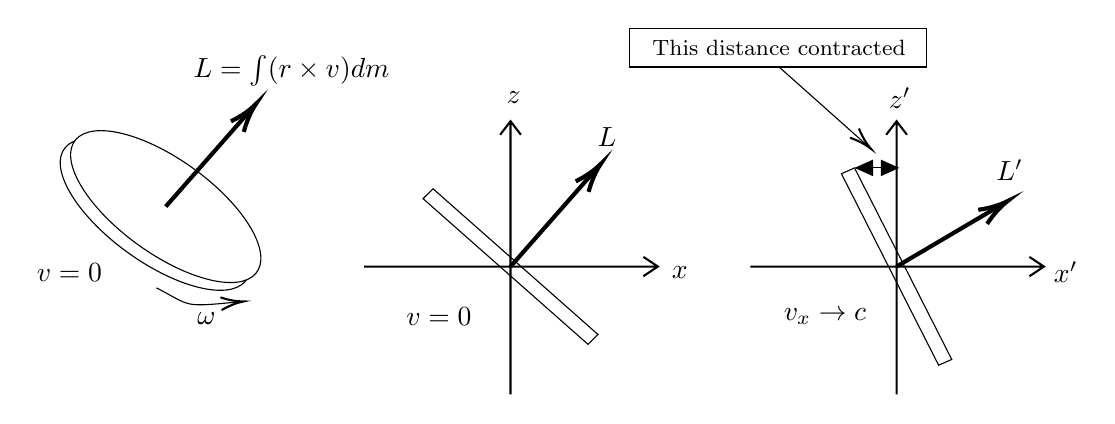
\begin{tikzpicture}[x=0.75pt,y=0.7pt,yscale=-1,xscale=1]
%uncomment if require: \path (0,300); %set diagram left start at 0, and has height of 300

%Shape: Ellipse [id:dp6696584947764774] 
\draw   (105.99,95.55) .. controls (114.14,85.31) and (140.18,92.46) .. (164.14,111.53) .. controls (188.1,130.6) and (200.92,154.36) .. (192.77,164.6) .. controls (184.62,174.85) and (158.58,167.7) .. (134.62,148.63) .. controls (110.66,129.56) and (97.84,105.8) .. (105.99,95.55) -- cycle ;
%Shape: Ellipse [id:dp8843951455763316] 
\draw  [fill={rgb, 255:red, 255; green, 255; blue, 255 }  ,fill opacity=1 ] (110.99,91.55) .. controls (119.14,81.31) and (145.18,88.46) .. (169.14,107.53) .. controls (193.1,126.6) and (205.92,150.36) .. (197.77,160.6) .. controls (189.62,170.85) and (163.58,163.7) .. (139.62,144.63) .. controls (115.66,125.56) and (102.84,101.8) .. (110.99,91.55) -- cycle ;
%Straight Lines [id:da6714691596952527] 
\draw [line width=1.5]    (154.38,126.08) -- (196,75.35) ;
\draw [shift={(197.9,73.03)}, rotate = 489.37] [color={rgb, 255:red, 0; green, 0; blue, 0 }  ][line width=1.5]    (14.21,-4.28) .. controls (9.04,-1.82) and (4.3,-0.39) .. (0,0) .. controls (4.3,0.39) and (9.04,1.82) .. (14.21,4.28)   ;

%Curve Lines [id:da608409716212424] 
\draw    (149.9,168.03) .. controls (167.54,177.83) and (162.13,178.03) .. (190.14,175.21) ;
\draw [shift={(191.9,175.03)}, rotate = 534.29] [color={rgb, 255:red, 0; green, 0; blue, 0 }  ][line width=0.75]    (10.93,-3.29) .. controls (6.95,-1.4) and (3.31,-0.3) .. (0,0) .. controls (3.31,0.3) and (6.95,1.4) .. (10.93,3.29)   ;

%Shape: Rectangle [id:dp2988248655701031] 
\draw  [fill={rgb, 255:red, 255; green, 255; blue, 255 }  ,fill opacity=1 ] (283.18,116.89) -- (362.64,192.09) -- (357.82,197.17) -- (278.36,121.98) -- cycle ;
%Shape: Axis 2D [id:dp3998228460871881] 
\draw [line width=0.75]  (250,157.03) -- (391.5,157.03)(320.5,82) -- (320.5,223.03) (384.5,152.03) -- (391.5,157.03) -- (384.5,162.03) (315.5,89) -- (320.5,82) -- (325.5,89)  ;
%Straight Lines [id:da08204495575914073] 
\draw [line width=1.5]    (320.5,157.03) -- (362.12,106.31) ;
\draw [shift={(364.02,103.99)}, rotate = 489.37] [color={rgb, 255:red, 0; green, 0; blue, 0 }  ][line width=1.5]    (14.21,-4.28) .. controls (9.04,-1.82) and (4.3,-0.39) .. (0,0) .. controls (4.3,0.39) and (9.04,1.82) .. (14.21,4.28)   ;

%Shape: Rectangle [id:dp9756203932975158] 
\draw  [fill={rgb, 255:red, 255; green, 255; blue, 255 }  ,fill opacity=1 ] (486.24,106.1) -- (533.08,204.97) -- (526.76,207.96) -- (479.92,109.1) -- cycle ;
%Shape: Axis 2D [id:dp2253494066411521] 
\draw [line width=0.75]  (436,157.03) -- (577.5,157.03)(506.5,82) -- (506.5,223.03) (570.5,152.03) -- (577.5,157.03) -- (570.5,162.03) (501.5,89) -- (506.5,82) -- (511.5,89)  ;
%Straight Lines [id:da26681235965231986] 
\draw [line width=1.5]    (506.5,157.03) -- (557.46,124.84) ;
\draw [shift={(560,123.23)}, rotate = 507.72] [color={rgb, 255:red, 0; green, 0; blue, 0 }  ][line width=1.5]    (14.21,-4.28) .. controls (9.04,-1.82) and (4.3,-0.39) .. (0,0) .. controls (4.3,0.39) and (9.04,1.82) .. (14.21,4.28)   ;

%Straight Lines [id:da2736459794596652] 
\draw    (489.24,106.1) -- (504.8,106.1) ;
\draw [shift={(507.8,106.1)}, rotate = 180] [fill={rgb, 255:red, 0; green, 0; blue, 0 }  ][line width=0.08]  [draw opacity=0] (8.93,-4.29) -- (0,0) -- (8.93,4.29) -- cycle    ;
\draw [shift={(486.24,106.1)}, rotate = 0] [fill={rgb, 255:red, 0; green, 0; blue, 0 }  ][line width=0.08]  [draw opacity=0] (8.93,-4.29) -- (0,0) -- (8.93,4.29) -- cycle    ;
%Straight Lines [id:da8576239603286319] 
\draw    (450.13,54.23) -- (492.69,94.85) ;
\draw [shift={(494.13,96.23)}, rotate = 223.67000000000002] [color={rgb, 255:red, 0; green, 0; blue, 0 }  ][line width=0.75]    (10.93,-3.29) .. controls (6.95,-1.4) and (3.31,-0.3) .. (0,0) .. controls (3.31,0.3) and (6.95,1.4) .. (10.93,3.29)   ;


% Text Node
\draw (174,184) node    {$\omega $};
% Text Node
\draw (108,160) node    {$v=0$};
% Text Node
\draw (402,160) node    {$x$};
% Text Node
\draw (322,70) node    {$z$};
% Text Node
\draw (215,56) node    {$L=\int ( r\times v) dm$};
% Text Node
\draw (367,90) node    {$L$};
% Text Node
\draw (286,183) node    {$v=0$};
% Text Node
\draw (588,160) node    {$x'$};
% Text Node
\draw (508,70) node    {$z'$};
% Text Node
\draw (561,107) node    {$L^{\prime }$};
% Text Node
\draw (472,183) node    {$v_{x}\rightarrow c$};
% Text Node
\draw    (378,34) -- (521,34) -- (521,54) -- (378,54) -- cycle  ;
\draw (449.87,44) node  [font=\footnotesize] [align=left] {This distance contracted};


\end{tikzpicture}
    \caption{Spinning disk}
    \label{fig:spinning-disk}
\end{figure}
The closer the disk gets to the speed of light, the more the disk surface appears in the observer's frame to align normal to the velocity direction. In the rest frame translating with the disk itself, the disk still appears aligned in the original way. In the observer's frame, though, the angular momentum L appears to turn toward the direction of the velocity becoming $L^{\prime}$. The greater the speed, the greater this turning. At light speed, $L^{\prime}$ and $v$ become parallel.

Quantum mechanically, then, \bluep{at high speed, a particle's angular momentum (spin) magnitude remains unchanged, but its direction appears to us in our frame to realign itself closer to that of the translational velocity vector.}

Mathematically, these kinds of relativistic complications are incorporated into the form of the spinors $u_{r}(\mathrm{p})$ and $v_{r}(\mathrm{p})$ (by their dependence on 3 -momentum and thus ultimately, on velocity) and by how they are combined to form more general spin states.

\begin{qt}
\redp{Note that the spinor components are actually dependent on particle velocity, rather than momentum, by the following logic.} Energy and momentum are expressed (in non-natural units to make it easier to understand)
$$
E=\frac{m c^{2}}{\sqrt{1-v^{2} / c^{2}}} \quad p^{i}=\frac{m v^{i}}{\sqrt{1-v^{2} / c^{2}}}
$$
so in the coefficient and spinor components of the Dirac spinor (\ref{four-spinors}) the mass $m$ drops out. This leaves them a function solely of velocity.
\end{qt}

\subsubsection{What happens when the particle is not stationary}
Note what happens to the spin as seen by us, for an electron whose spin is represented solely by
$u_{1},$ but has $p^{1} \neq 0,$ with $p^{2}=p^{3}=0$ in our frame (the lab.)
$$
\Sigma_{3}\left|\psi^{(1)}\right\rangle=\frac{1}{2}\left[\begin{array}{cccc}
{1} & {} \\
{} & {-1} \\
{} & {} & {1} \\
{} & {} & {}&{-1}
\end{array}\right] \frac{E+m}{2 m}\left(\begin{array}{c}
{1} \\
{0} \\
{0} \\
{\frac{p^{1}}{E+m}}
\end{array}\right) e^{-f p x}=\frac{1}{2} \sqrt{\frac{E+m}{2 m}}\left(\begin{array}{c}
{1} \\
{0} \\
{0} \\
{\frac{-p^{1}}{E+m}}
\end{array}\right) e^{-i p x} \neq \frac{1}{2}\left|\psi^{(1)}\right\rangle
$$
\textbf{\redp{$u_1$ for a non-translating electron has spin up, but $u_1$ for an electron with high trnasverse velocity is not an up eigenstate.}}

Now consider $u_1$ representing an electron traveling in the $z$ direction instead of the x direction
$$
\Sigma_{3}\left|\psi^{(1)}\right\rangle=\frac{1}{2}\left[\begin{array}{cccc}
{1} \\
{} & {-1} \\
{} & {} & {1} \\
{} & {} & {} & {-1}
\end{array}\right]\sqrt{\frac{E+m}{2 m}}\left(\begin{array}{c}
{1} \\
{0} \\
{p^{3}} \\
{\frac{p^{3}}{E+m}} \\
{0}
\end{array}\right) e^{-t p x}=\frac{1}{2} \sqrt{\frac{E+m}{2 m}}\left(\begin{array}{c}
{1} \\
{0} \\
{\frac{p^{3}}{E+m}} \\
{0}
\end{array}\right) e^{-i p x}=\frac{1}{2}\left|\psi^{(1)}\right\rangle
$$
This electron, represented by $u_{1},$ is an up eigenstate as it moves, just as it was when it was at rest. Relativistically, this makes sense, as the plane of a spinning disk with $\mathbf{L}$ aligned in the direction of $\mathbf{p}$ would not appear to turn as $\mathbf{p}$ increased from zero to a relativistic value.

\redp{\textbf{In general, boosts in the spin axis direction leave $u_{1}, u_{2}, v_{2}$ and $v_{1}$ in the same spin eigenstates as they would be at rest. Boosts in other directions take them out of these spin eigenstates.}}

\begin{mybox}
\textbf{The four-spinors span the 4D spinor space}

By analogy, we can surmise that the four Dirac spinors $u_{1}, u_{2}, v_{2}$ and $v_{1}$ of (\ref{four-spinors}) span the $\mathrm{RQM}$ 4D spinor space of all possible spins and momenta, and thus, are basis vectors for that space. Our RQM general solution (\ref{general-Dirac-state}) contains within it all possible relativistic spin states.

More mathematically, we should know that a $4 \mathrm{D}$ space is spanned by four column vectors, where these vectors are all independent of one another. Generally. the vector solutions of an eigenvalue problem, which is what the Dirac equation solutions are, are independent and complete, and thus we can conclude, span the space. They can be used as basis vectors.
\end{mybox}
\subsubsection{General RQM solution contains all possible spin directions}
In (\ref{general-Dirac-state}), different coefficients $C_{1}(\mathbf{p})$ and $\mathcal{C}_{2}(\mathbf{p})$ will yield different spin states for C type particles. And different coefficients $D^{\dagger}_{1(\mathbf{p})}$ and $D^{\dagger}_{2(\mathbf{p})}$ will yield different spin states for $D$ type particles.

To see how this works, we consider how each of the four states shown below can be represented by their respective terms in the general particle state solution (\ref{general-Dirac-state}). 
\begin{figure}[H]
    \centering
\tikzset{every picture/.style={line width=0.75pt}} %set default line width to 0.75pt        

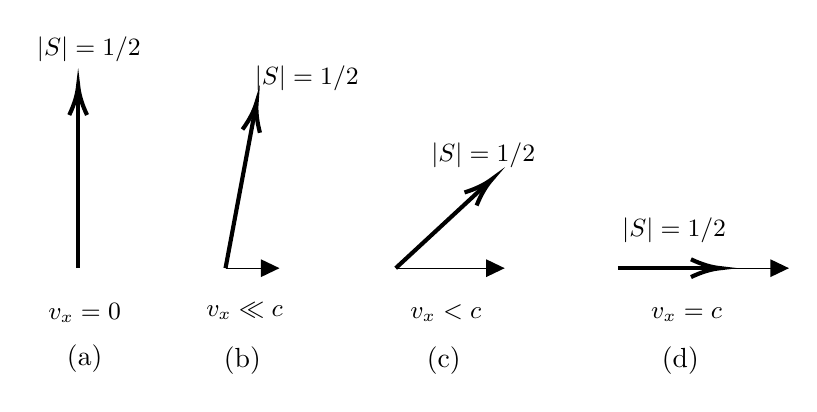
\begin{tikzpicture}[x=0.75pt,y=0.75pt,yscale=-1,xscale=1]
%uncomment if require: \path (0,300); %set diagram left start at 0, and has height of 300

%Straight Lines [id:da533603137195499] 
\draw [line width=1.5]    (79.87,190.5) -- (79.87,105.5) ;
\draw [shift={(79.87,102.5)}, rotate = 450] [color={rgb, 255:red, 0; green, 0; blue, 0 }  ][line width=1.5]    (14.21,-4.28) .. controls (9.04,-1.82) and (4.3,-0.39) .. (0,0) .. controls (4.3,0.39) and (9.04,1.82) .. (14.21,4.28)   ;

%Straight Lines [id:da31466198885223695] 
\draw    (150.87,190.5) -- (173.87,190.5) ;
\draw [shift={(176.87,190.5)}, rotate = 180] [fill={rgb, 255:red, 0; green, 0; blue, 0 }  ][line width=0.08]  [draw opacity=0] (8.93,-4.29) -- (0,0) -- (8.93,4.29) -- cycle    ;

%Straight Lines [id:da6431925700861189] 
\draw [line width=1.5]    (150.87,190.5) -- (165.31,113.45) ;
\draw [shift={(165.87,110.5)}, rotate = 460.62] [color={rgb, 255:red, 0; green, 0; blue, 0 }  ][line width=1.5]    (14.21,-4.28) .. controls (9.04,-1.82) and (4.3,-0.39) .. (0,0) .. controls (4.3,0.39) and (9.04,1.82) .. (14.21,4.28)   ;

%Straight Lines [id:da8282450907912188] 
\draw    (232.87,190.5) -- (282.37,190.5) ;
\draw [shift={(285.37,190.5)}, rotate = 180] [fill={rgb, 255:red, 0; green, 0; blue, 0 }  ][line width=0.08]  [draw opacity=0] (8.93,-4.29) -- (0,0) -- (8.93,4.29) -- cycle    ;

%Straight Lines [id:da09697600465348566] 
\draw [line width=1.5]    (232.87,190.5) -- (277.16,149.54) ;
\draw [shift={(279.37,147.5)}, rotate = 497.24] [color={rgb, 255:red, 0; green, 0; blue, 0 }  ][line width=1.5]    (14.21,-4.28) .. controls (9.04,-1.82) and (4.3,-0.39) .. (0,0) .. controls (4.3,0.39) and (9.04,1.82) .. (14.21,4.28)   ;

%Straight Lines [id:da13695386046952507] 
\draw    (339.87,190.5) -- (419.33,190.5) ;
\draw [shift={(422.33,190.5)}, rotate = 180] [fill={rgb, 255:red, 0; green, 0; blue, 0 }  ][line width=0.08]  [draw opacity=0] (8.93,-4.29) -- (0,0) -- (8.93,4.29) -- cycle    ;

%Straight Lines [id:da04790853968035602] 
\draw [line width=1.5]    (339.87,190.5) -- (386.33,190.5) ;
\draw [shift={(389.33,190.5)}, rotate = 180] [color={rgb, 255:red, 0; green, 0; blue, 0 }  ][line width=1.5]    (14.21,-4.28) .. controls (9.04,-1.82) and (4.3,-0.39) .. (0,0) .. controls (4.3,0.39) and (9.04,1.82) .. (14.21,4.28)   ;


% Text Node
\draw (85,85.07) node  [font=\small]  {$|S|=1/2$};
% Text Node
\draw (83,212.07) node  [font=\small]  {$v_{x} =0$};
% Text Node
\draw (160,211.07) node  [font=\small]  {$v_{x} \ll c$};
% Text Node
\draw (257,212.07) node  [font=\small]  {$v_{x} < c$};
% Text Node
\draw (373,213.07) node  [font=\small]  {$v_{x} =c$};
% Text Node
\draw (190,99.07) node  [font=\small]  {$|S|=1/2$};
% Text Node
\draw (275,136.07) node  [font=\small]  {$|S|=1/2$};
% Text Node
\draw (367,172.07) node  [font=\small]  {$|S|=1/2$};
% Text Node
\draw (83,234.07) node   [align=left] {(a)};
% Text Node
\draw (159,235.07) node   [align=left] {(b)};
% Text Node
\draw (256,235.07) node   [align=left] {(c)};
% Text Node
\draw (370,235.07) node   [align=left] {(d)};


\end{tikzpicture}

    \caption{Effect of Transverse Velocity on Dirac Particle Spin}
    \label{fig:transverse-velocity-effect}
\end{figure}

In general, for $j=a,b,c,d$, the four states shown (for a C type particle) in the figure are
\begin{equation}
\left|\psi_{(j)}\right\rangle=\sqrt{\frac{m}{V E_{p_{j}}}}\left(C_{1}\left(p_{j}\right) u_{1}\left(p_{j}\right)+C_{2}\left(p_{j}\right) u_{2}\left(p_{j}\right)\right) e^{-i p_{j} x}
\label{psi-abcd}
\end{equation}
Not that we have a particle here (so no $D$ type terms), and $\mathbf{p}_j$ is known. State (a) there is effectively spin up with $\mathrm{p}_{\mathrm{a}}=0$, so
\begin{equation}
\left|\psi_{(a)}\right\rangle=\sqrt{\frac{m}{V E_{p_{a}}}} C_{1}(0) u_{1}(0) e^{-i p_{a} x}=\sqrt{\frac{m}{V E_{\mathrm{p}_{a}}}} \sqrt{\frac{E_{\mathrm{p}_{a}}+m}{2 m}}\left(\begin{array}{l}
{\mathrm{I}} \\
{0} \\
{0} \\
{0}
\end{array}\right) e^{-i p_{a} x}
\end{equation}
which is an eigenstate of $\Sigma_3$. So for state (a), $|\psi_a\rangle$ has $C_1=1$ and $C_2=0$.

For the last state (d), where the particle is traveling at the speed of light, (\ref{psi-abcd}) becomes an eigenstate of $\Sigma_1$ with eigenvalue $1/2$,
$$
\left|\psi_{(d)}\right\rangle=\sqrt{\frac{m}{V E_{\mathrm{p}_{d}}}} C_{1}(\infty) u_{1}(\infty) e^{-i p_{d} x}+\sqrt{\frac{m}{V E_{\mathrm{p} d}}} C_{2}(\infty) u_{2}(\infty) e^{-i p_{d} x}
$$
$$
=\sqrt{\frac{m}{V E_{\mathrm{p}_{d}}}} \sqrt{\frac{E_{\mathrm{p}_{d}}+m}{2 m}}\left(\begin{array}{l}
{1} \\
{1} \\
{1} \\
{1}
\end{array}\right) e^{-i p_{d} x}
$$
where here, we must have $C_1=C_2=1$. (in the normalized version, $C_1=C_2=1/\sqrt{2}$).For "in between" states $(b)$ and $(c), C_{1}$ and $C_{2}$ would have other values. The bottumline is:\redp{$\mathbf{p}$ determines $u_{1,2}$ and then spin is represented by correct linear combination of $u_1$ and $u_2$}. Note that \bluep{we can never have a relativistic state where the spin vector and $\mathbf{p}$ are at right angles.}

Note that $u_{1}$ and $u_{2}$ actually exist in spinor space (they are spinor space basis vectors in that space), but they correspond to directions in physical space. For example, in the at-rest system, $u_1$ represents spin up and so can be visualized as a spatial vector that points in the $+z$ direction. Similarly, in the at-rest system, $u_{2}$ represents spin down, so can be visualized as a vector pointing in the $-z$ direction. 
\begin{qt}
\underline{Summary}

1. $u_{1}(\mathrm{p}) e^{-i p x}$ and  $u_{2}(\mathrm{p}) e^{-i p x}$ is each always an eigenstate of the Dirac equation (for any $\mathbf{p}$)

2. $u_{1}(\mathrm{p}) e^{-i p x}$ and $u_{2}(\mathrm{p}) e^{-i p x}$ is each sometimes an eigenstate of $z$ spin, i.e. of $\Sigma_{3}\left(\text { for } \mathbf{p}=0 \text { or }=p^{3} \mathbf{i}_{3}\right)$

3. $u_{1}(\mathbf{p}) e^{-i p x}$ and $u_{2}(\mathbf{p}) e^{-i p x}$ are always basis vectors for any general state $|\psi\rangle$ (for any $\mathbf{p}$ )

4. $u_{1}(p)$ and $u_{2}(p)$ is each sometimes an eigenstate of $z$ spin, i.e. of $\Sigma_{3}$ for $\mathbf{p}=0$ or$=p^{3} \mathbf{i}_{3}$)

5. $u_{1}(\mathbf{p})$ and $u_{2}(\mathbf{p})$ are always basis vectors in $4 \mathrm{D}$ spinor space (for any $\mathbf{p}$) 

6. \textbf{$u_{1}(\mathrm{p})$ and $u_{2}(\mathrm{p})$ change orientation, as visualized in physical space, as $\mathrm{p}$ changes.}

7. Spin S (often in relativity as $\Sigma$ ) changes direction with p, but differently than $u_{1}$ and $u_{2}$
\end{qt}
Any general spin state $u$ can be represented as a linear combination of $u_{1}$ and  $u_{2}$ (for any $\mathbf{p}$)
$$
u(\mathrm{p})=C_{1}(\mathrm{p}) u_{1}(\mathrm{p})+C_{2}(\mathrm{p}) u_{2}(\mathrm{p})
$$
Any general particle state includes a spin part plus a spacetime part(for any given $\mathbf{p}$):
$$
\left|\psi_{\mathfrak{p}}\right\rangle=\sqrt{\frac{m}{2 V E_{\mathrm{p}}}} u(\mathbf{p}) e^{-i p x}=\sqrt{\frac{m}{2 V E_{\mathrm{p}}}}\left(C_{1}(\mathrm{p}) u_{1}(\mathrm{p}) e^{-i p x}+C_{2}(\mathrm{p}) u_{2}(\mathrm{p}) e^{-i p x}\right)
$$
\subsection{RQM Helicity operator}
For massless particles ($v=c$), the velocity vector must perfectly align with the spin vector. This alignment is called \textbf{perfect helicity}. In general, if the spin axis (using the right-hand rule), of a particle is in the direction of $v$ one
says the particle has \textbf{positive helicity}. If spin points in the direction of $- v$, the particle has \textbf{negative helicitv}. 

The degree  of helicity a particle has be define in terms of the angle between the spin vector and the velocity vector. It is maximum if that angle is zero.\textbf{ The dot product of the spin vector with a unit vector in the $\mathbf{p}$ (or equivalently, the $v$) direction has come to be the mathematical definition of helicity}.

\bluep{Our spin operator $\Sigma$ in RQM plays the role of a 3-vector in physical space that points in the direction of spin.} The inner product in physical space of the spin operator $\Sigma$ and the unit vector in the $\mathbf{p}$ direction would then be \textbf{helicity operator}:
\begin{qt}
\begin{equation}
\Sigma_{p}=\Sigma \cdot i_{p}=\Sigma \cdot \frac{p}{|p|}=\Sigma_{1} \frac{p^{1}}{|p|}+\Sigma_{2} \frac{p^{2}}{|p|}+\Sigma_{3} \frac{p^{3}}{|p|}
\label{helicity-operator}
\end{equation}
(\ref{helicity-operator}) is a $4\times4$ matrix in spinor space because each $\Sigma_i$ is a matrix. (\ref{helicity-operator}) is a scalar in physical space because it is the inner product of two vectors.
\end{qt}
\begin{example}
Consider a case where a particle is in the first eigenstate of (\ref{four-spinors}), and if $p^3\neq0$, we have
$$
\Sigma \cdot \frac{\mathbf{p}}{|\mathbf{p}|}\left|\psi^{(1)}\right\rangle=\Sigma_{3} \underbrace{\frac{p^{3}}{|\mathbf{p}|}}_{=1}\left|\psi^{(1)}\right\rangle=\frac{1}{2}\left[\begin{array}{cccc}
{1} \\
{} & {-1} \\
{} & {} & {1} \\
{} & {} & {} & {-1}
\end{array}\right]\sqrt{\frac{E+m}{2 m}}\left(\begin{array}{c}
{1} \\
{0} \\
{\frac{p^3}{E+m}} \\
{0}
\end{array}\right)e^{-ipx}=\frac{1}{2}\left|\psi^{(1)}\right\rangle
$$
\end{example}
\begin{example}
Note that if $p^3$ were negative (-z direction)
$$
\Sigma_{3}\left|\psi^{(1)}\right\rangle=\frac{1}{2}\left[\begin{array}{cccc}
{1} \\
{} & {-1} \\
{} & {} & {1} \\
{} & {} & {} & {-1}
\end{array}\right]\sqrt{\frac{E+m}{2 m}}\left(\begin{array}{c}
{1} \\
{0} \\
{\frac{p^{3}}{E+m}} \\
{0}
\end{array}\right) e^{-i p x}=\frac{1}{2}\left|\psi^{(1)}\right\rangle
$$
but
$$
\Sigma \cdot \frac{\mathbf{p}}{|\mathbf{p}|}\left|\psi^{(1)}\right\rangle=\Sigma_{3} \underbrace{\frac{p^{3}}{|\mathbf{p}|}}_{=-1}\left|\psi^{(1)}\right\rangle=-\frac{1}{2}\left|\psi^{(1)}\right\rangle
$$
\end{example}
In general, a $+1 / 2$ helicity state for spinors means the spin is in the direction of $p$; a $-1 / 2$ helicity eigenvalue means spin is in the direction of $-p$.

\section{The Dirac Equation in QFT}
The Dirac equation for fields (where we will, as with scalar fields, work in the Heisenberg picture), is
\begin{equation}
\left(i \gamma^{\mu} \partial_{\mu}-m\right) \psi=0
\end{equation}
Its eigensolutions
\begin{equation}
\psi^{(1)}=u_{1} e^{-i p x} \quad \psi^{(2)}=u_{2} e^{-i p x} \quad \psi^{(3)}=v_{2} e^{i p x} \quad \psi^{(4)}=v_{1} e^{i p x}
\end{equation}
\textbf{\underline{The adjoint Dirac equation for fields is}}
\begin{equation}
i \partial_{\mu} \bar{\psi} \gamma^{\mu}+m \bar{\psi}=0
\end{equation}
with adjoint eigensolutions
\begin{equation}
\bar{\psi}=\psi^{\dagger} \gamma^{0} \rightarrow \bar{\psi}^{(1)}=u_{1}^{\dagger} \gamma_{e}^{0} e^{i p x}=\bar{u}_{\mathrm{l}} e^{i p x} \quad \bar{\psi}^{(2)}=\bar{u}_{2} e^{i \phi x} \quad \bar{\psi}^{(3)}=\bar{v}_{2} e^{-i \varphi x} \quad \bar{\psi}^{(4)}=\bar{v}_{1} e^{-\dot{\varphi} x}
\end{equation}
\begin{qt}
the general discrete plane wave solutions are
\begin{equation}
\begin{aligned}
\psi &=\sum_{r, \mathbf{p}} \sqrt{\frac{m}{V E_{\mathrm{p}}}}\left(c_{r}(\mathbf{p}) u_{r}(\mathbf{p}) e^{-i p x}+d_{r}^{\dagger}(\mathbf{p}) v_{r}(\mathbf{p}) e^{i p x}\right) \\
&=\quad \psi^{+} \quad+\quad \psi^{-}
\end{aligned}
\end{equation}
\begin{equation}
\begin{aligned}
&\bar{\psi}=\sum_{r, p} \sqrt{\frac{m}{V E_{p}}}\left(d_{r}(p) \bar{v}_{r}(p) e^{-i p x}+c_{r}^{\dagger}(p) \bar{u}_{r}(p) e^{i p x}\right)\\
&=\quad \bar{\psi}^{+} \quad+\quad \bar{\psi}^{-}
\end{aligned}
\end{equation}
\end{qt}
The general continuous plane wave solutions are
\begin{equation}
\begin{aligned}
&\psi=\sum_{r} \sqrt{\frac{m}{(2 \pi)^{3}}} \int \frac{d^{3} \mathbf{p}}{\sqrt{E_{p}}}\left(c_{r}(\mathbf{p}) u_{r}(\mathbf{p}) e^{-i p x}+d_{r}^{\dagger}(\mathbf{p}) v_{r}(\mathbf{p}) e^{i p x}\right)\\
&\bar{\psi}=\sum_{r} \sqrt{\frac{m}{(2 \pi)^{3}}} \int \frac{d^{3} \mathbf{p}}{\sqrt{E_{p}}}\left(d_{r}(\mathbf{p}) \bar{v}_{r}(\mathbf{p}) e^{-i p x}+c_{r}^{\dagger}(\mathbf{p}) \bar{u}_{r}(\mathbf{p}) e^{i p x}\right)
\end{aligned}
\end{equation}
\begin{qt}
the Lagrangian ( density) for free spinor fields to be
\begin{equation}
\mathcal{L}_{0}^{1/2}=\bar{\psi}\left(i \gamma^{\alpha} \partial_{\alpha}-m\right) \psi
\end{equation}
Conjugate momenta for $\psi$ and $\bar{\psi}$ are
\begin{equation}
\pi^{1 / 2}=\frac{\partial \mathcal{L}_{0}^{1 / 2}}{\partial \psi_{0}}=i \psi \gamma^{0}=i \psi^{\dagger} \gamma^{\dagger} \gamma^{0}=i \psi^{\dagger}
\end{equation}
\begin{equation}
\bar{\pi}^{1 / 2}=\frac{\partial \mathcal{L}_{0}^{1 / 2}}{\partial \bar{\psi}_{, 0}}=0
\end{equation}
The Dirac Hamiltonian density can be found from the Legendre transformation as
\begin{equation}
\begin{aligned}
\mathcal{H}_{0}^{1 / 2} &=\pi^{1 / 2} \dot{\psi}+\bar{\pi}^{1 / 2} \dot{\bar{\psi}}-\mathcal{L}_{0}^{1 / 2}=i \psi^{\dagger} \dot{\psi}-\mathcal{L}_{0}^{1 / 2}=i \underbrace{\psi^{\dagger} \gamma^{0}}_{\bar{\psi}} \gamma^{0} \dot{\psi}-\mathcal{L}_{0}^{1 / 2} \\
&=i \bar{\psi} \gamma^{0} \dot{\psi}\underbrace{-i \bar{\psi} \gamma^{0} \dot{\psi}-i \bar{\psi} \gamma^{i} \partial_{i} \psi}_{-i\bar{\psi}\gamma^{\alpha}\partial_{\alpha}\psi}+m \bar{\psi} \psi=-i \bar{\psi} \gamma^{i} \partial_{i} \psi+m \bar{\psi} \psi
\end{aligned}
\end{equation}
\end{qt}
\section{Anti-commutation Relations for Dirac Fields}
\begin{qt}
\begin{equation}
    \left[c_{r}(\mathbf{p}), c_{s}^{\dagger}\left(\mathbf{p}^{\prime}\right)\right]_{+}=\left[d_{r}(\mathbf{p}), d_{s}^{\dagger}\left(\mathbf{p}^{\prime}\right)\right]_{+}=\delta_{r S} \delta_{\mathbf{p p}^{\prime}}(\text { discrete }) ;=\delta_{r s} \delta(\mathbf{p - p ^ { \prime }})(\text { continuous })
\end{equation}
All other anti-commutators between coefficients equal zero.
\end{qt}
\section{The Dirac Hamiltonian in QFT}
Similar to what we did for scalar fields, we find the Dirac Hamiltonian by integrating the Dirac Hamiltonian density over all space (a volume V containing the discrete solutions, which we can make as large as we like), i.e.,
\begin{equation}
H_{0}^{1 / 2}=\int \mathcal{H}_{0}^{1 / 2} d^{3} x=\int\left(-i \bar{\psi} \gamma^{i} \partial_{i} \psi+m \bar{\psi} \psi\right) d^{3} x
\label{Dirac-Hamiltonian}
\end{equation}
we substitute the Dirac general solution into (\ref{Dirac-Hamiltonian}) to give
$$
\begin{aligned}
&H_{0}^{1 / 2}=\int\left(-i \bar{\psi} \gamma^{i} \partial_{i} \psi+m \bar{\psi} \psi\right) d^{3} x=\\
&\int\left(\sum_{r, p} \sqrt{\frac{m}{V E_{p}}}\left(d_{r}(p) \bar{v}_{r}(\mathbf{p}) e^{-i p x}+c_{r}^{\dagger}(\mathbf{p}) \bar{u}_{r}(\mathbf{p}) e^{i p x}\right)\right) \times
\end{aligned}
$$
$$
\left(-i \gamma^{i} \partial_{i}\right)\left(\sum_{s, p^{\prime}} \sqrt{\frac{m}{V E_{p^{\prime}}}}\left(c_{s}\left(\mathbf{p}^{\prime}\right) u_{s}\left(\mathbf{p}^{\prime}\right) e^{-i p^{\prime} x}+d_{s}^{\dagger}\left(\mathbf{p}^{\prime}\right) v_{s}\left(\mathbf{p}^{\prime}\right) e^{i p^{\prime} x}\right)\right) d^{3} x
$$
$$
+\int m\left(\sum_{r, p} \sqrt{\frac{m}{V E_{p}}}\left(d_{r}(p) \bar{v}_{r}(p) e^{-i p x}+c_{r}^{\dagger}(p) \bar{u}_{r}(p) e^{i p x}\right)\right) \times
$$
$$
\left(\sum_{s, \mathbf{p}^{\prime}} \sqrt{\frac{m}{V E_{\mathbf{p}^{\prime}}}}\left(c_{s}\left(\mathbf{p}^{\prime}\right) u_{s}\left(\mathbf{p}^{\prime}\right) e^{-i p^{\prime} x}+d_{s}^{\dagger}\left(\mathbf{p}^{\prime}\right) v_{s}\left(\mathbf{p}^{\prime}\right) e^{i \mathbf{p}^{\prime} \cdot x}\right)\right) d^{3} x
$$
The first of the two integrals above becomes
$$
 \int\left(\sum_{r, \mathbf{p}} \sqrt{\frac{m}{V E_{p}}}d_{r}(\mathbf{p}) \bar{v}_{r}(\mathbf{p}) e^{-i\left(E_{p} t-p^{i} x^{i}\right)}\right)\left(\sum_{s, p^{\prime}} \sqrt{\frac{m}{V E_{p^{\prime}}}} c_{s}\left(\mathbf{p}^{\prime}\right) \gamma^{i} \underbrace{p^{\prime i}}_{\text { from }\partial_i} u_{s}\left(\mathbf{p}^{\prime}\right) e^{-i\left(E_{p^{\prime}}-p^{\prime i} x^{i}\right)}\right)d^3x
$$
$$
+\int\left(\sum_{r, \mathrm{p}} \sqrt{\frac{m}{V E_{\mathrm{p}}}} d_{r}(\mathrm{p}) \bar{v}_{r}(\mathbf{p}) e^{-i\left(E_{\mathrm{p}} t-p^{i} x^{i}\right)}\right)\left(\sum_{s, p^{\prime}} \sqrt{\frac{m}{V E_{p^{\prime}}}} d_{s}^{\dagger}\left(p^{\prime}\right) \gamma^{i}\left(-p^{\prime i}\right) v_{s}\left(p^{\prime}\right) e^{i\left(E_{p^{\prime}}t-p^{\prime i} x^{i}\right)}\right) d^{3} x
$$
$$
+\int\left(\sum_{r, \mathrm{p}} \sqrt{\frac{m}{V E_{\mathrm{p}}}} c^{\dagger}_{r}(\mathrm{p}) \bar{u}_{r}(\mathbf{p}) e^{-i\left(E_{\mathrm{p}} t-p^{i} x^{i}\right)}\right)\left(\sum_{s, p^{\prime}} \sqrt{\frac{m}{V E_{p^{\prime}}}} c_{s}\left(p^{\prime}\right) \gamma^{i}\left(p^{\prime i}\right) u_{s}\left(p^{\prime}\right) e^{i\left(E_{p^{\prime}}t-p^{\prime i} x^{i}\right)}\right) d^{3} x
$$
$$
+\int\left(\sum_{r, \mathrm{p}} \sqrt{\frac{m}{V E_{\mathrm{p}}}} c^{\dagger}_{r}(\mathrm{p}) \bar{u}_{r}(\mathbf{p}) e^{-i\left(E_{\mathrm{p}} t-p^{i} x^{i}\right)}\right)\left(\sum_{s, p^{\prime}} \sqrt{\frac{m}{V E_{p^{\prime}}}} d^{\dagger}_{s}\left(p^{\prime}\right) \gamma^{i}\left(-p^{\prime i}\right) v_{s}\left(p^{\prime}\right) e^{i\left(E_{p^{\prime}}t-p^{\prime i} x^{i}\right)}\right) d^{3} x
$$
\redp{because an integral over all space of the oscillating function $e^{if(\mathbf{x})}$, where $f(\mathbf{x}\neq0)$ is zero. }So,in the first and last lines, only terms with $\mathbf{p}=-\mathbf{p}^{\prime}$ will survive. And in the $2^{\text {nd }}$ and $3^{\text {rd }}$ lines, only terms in $\mathbf{p}^{\prime}=\mathbf{p}$ will. We assume, as in $\mathrm{RQM},$ that \textbf{\redp{the order of spinors and coefficients (such as $c_{r} \text { and } d_{r}$) can be interchanged at will, but we must preserve the order of spinor entities as it represent matrix/vector multiplication in spinor space.}}
$$
+\int\left[\sum_{r, s, \mathbf{p}} \frac{m}{V E_{\mathbf{p}}} d_{r}(-\mathbf{p}) \bar{v}_{r}(-\mathbf{p}) \gamma^{i} p^{i} u_{s}(\mathbf{p}) c_{s}(\mathbf{p}) e^{-i 2 E_{p} t}\right] d^{j}
$$
$$
+\int\left(\sum_{r, s, \mathbf{p}} \frac{m}{V E_{\mathrm{p}}} d_{r}(\mathbf{p}) \bar{v}_{r}(\mathbf{p}) \gamma^{i}\left(-p^{i}\right) v_{s}(\mathbf{p}) d_{s}^{\dagger}(\mathbf{p})\right) d^{3} x
$$
$$
+\int\left(\sum_{r, s, \mathbf{p}} \frac{m}{V E_{p}} c_{r}^{\dagger}(\mathbf{p}) \bar{u}_{r}(\mathbf{p}) \gamma^{i} p^{i} u_{s}(\mathbf{p}) c_{s}(\mathbf{p})\right) d^{3} x
$$
$$
+\int\left(\sum_{r, s, \mathbf{p}} \frac{m}{V E_{p}} c_{r}^{\dagger}(-\mathbf{p}) \bar{u}_{r}(-\mathbf{p}) \gamma^{i}\left(-p^{i}\right) v_{s}(\mathbf{p}) d_{s}^{\dagger}(\mathbf{p}) e^{i 2 E_{p} t}\right) d^{3} x
$$
In similar fashion. the last two lines of the expansion of (\ref{Dirac-Hamiltonian}), representing the mass term in $H^{1/2}_0$, become
$$
\int\left(\sum_{r, s, \mathbf{p}} \frac{m}{V E_{p}} d_{r}(-\mathbf{p}) \bar{v}_{r}(-\mathbf{p}) m u_{s}(\mathbf{p}) c_{s}(\mathbf{p}) e^{-i 2 E_{p} t}\right) d^{3} x
$$
$$
\begin{aligned}
&+\int\left(\sum_{r, s, \mathbf{p}} \frac{m}{V E_{\mathbf{p}}} d_{r}(\mathbf{p}) \bar{v}_{r}(\mathbf{p}) m v_{s}(\mathbf{p}) d_{s}^{\dagger}(\mathbf{p})\right) d^{3} x\\
&+\int\left(\sum_{r, s, \mathbf{p}} \frac{m}{V E_{\mathrm{p}}} c_{r}^{\dagger}(\mathbf{p}) \bar{u}_{r}(\mathbf{p}) m u_{s}(\mathbf{p}) c_{s}(\mathbf{p})\right) d^{3} x
\end{aligned}
$$
$$
+\int\left(\sum_{r, s, \mathbf{p}} \frac{m}{V E_{\mathbf{p}}} c_{r}^{\dagger}(-\mathbf{p}) \bar{u}_{r}(-\mathbf{p}) m v_{s}(\mathbf{p}) d_{s}^{\dagger}(\mathbf{p}) e^{i 2 E_{\mathbf{p}} t}\right) d^{3} x
$$
\begin{mybox}
\textbf{Relationship for $u_{s}(\mathbf{p})$}

Consider the Dirac equation and a single eigensolution to it having 3 -momentum p and spin $s$
$$
\left(i \gamma^{\mu} \partial_{\mu}-m\right) \psi=(i \not \partial-m) \psi=0 \quad \text { with } \quad \psi=c_{\underline{s}}(\mathbf{p}) u_{\underline{s}}(\mathbf{p}) e^{-i p x}
$$
$$
\left(\gamma^{\mu} p_{\mu}-m\right) c_{\underline{s}}(\mathbf{p}) u_{\underline{s}}(\mathbf{p}) e^{-i p x}=(\not p-m) c_{\underline{s}}(\mathbf{p}) u_{\underline{s}}(\mathbf{p}) e^{-i p x}=0
$$
\textbf{Neither $c_{s}(p)$ nor the exponential equal zero, so the remaining factors must equal zero}, thus
$$
\left(\gamma^{\mu} p_{\mu}-m\right) u_{s}(\mathbf{p})=(\not p-m) u_{s}(\mathbf{p})=0
$$
Now from the complex conjugate transpose of (\ref{coefficient-orthogonality}), where r and s are dummy variables and thus interchangeable and the relation holds for any $\mathbf{p}$, including $-\mathbf{p}$,
$$
\begin{aligned}
u_{r}^{\dagger}(\mathbf{p}) v_{s}(-\mathbf{p})=0 & \rightarrow v_{s}^{\dagger}(-\mathbf{p}) u_{r}(\mathbf{p})=0 \rightarrow v_{r}^{\dagger}(-\mathbf{p}) u_{s}(\mathbf{p})=0 \\
v_{r}^{\dagger}(-\mathbf{p}) \gamma^{0} \gamma^{0} u_{s}(\mathbf{p})=0 & \rightarrow \bar{v}_{r}(-\mathbf{p}) \gamma^{0} u_{s}(\mathbf{p})=0 \rightarrow \bar{v}_{r}(-\mathbf{p}) \gamma^{0} p_{0} u_{s}(\mathbf{p})=0
\end{aligned}
$$
And thus,
$$
\bar{v}_{r}(-\mathrm{p}) \gamma^{i} p^{i} u_{s}(\mathrm{p})=\bar{v}_{r}(-\mathrm{p}) \gamma^{i}\left(-p_{i}\right) u_{s}(\mathrm{p})-\bar{v}_{r}(-\mathrm{p}) \gamma^{0} p_{0} u_{s}(\mathrm{p})=-\bar{v}_{r}(-\mathrm{p}) \underbrace{\gamma^{\mu} p_{\mu}}_{\not p} u_{s}(\mathrm{p})
$$
When we then use the RHS instead of the LHS of the equation above, we get
$$
-\int\left(\sum_{r, s, \mathbf{p}} \frac{m}{V E_{\mathbf{p}}} d_{r}(-\mathbf{p})(\bar{v}_{r}(-\mathbf{p})\underbrace{(\not p-m)u_s(\mathbf{p})}_{=0} c_{s}(\mathbf{p}) e^{-i 2 E_{p} t}\right) d^{3} x=0
$$
\end{mybox}
Recall that 
$$
v_{r}^{\dagger}(\mathbf{p}) v_{s}(\mathbf{p})=\bar{v}_{r}(\mathbf{p}) \gamma^{0} v_{s}(\mathbf{p})=\frac{E_{p}}{m} \delta_{r s}=\frac{p_{0}}{m} \delta_{r s}
$$
we have
$$
\bar{v}_{r}(\mathbf{p}) \gamma^{0} p_{0} v_{s}(\mathbf{p})=\frac{\left(p_{0}\right)^{2}}{m} \delta_{r s}=\frac{E_{p}^{2}}{m} \delta_{r s}
$$
Adding the integrals above, and using the relationship in the box, we find
\begin{equation}
\begin{aligned}
&\int\left(\sum_{r, s, \mathbf{p}} \frac{m}{V E_{p}} d_{r}(\mathbf{p}) \bar{v}_{r}(\mathbf{p})\left(-\gamma^{i} p^{i}+m\right) v_{s}(\mathbf{p}) d_{s}^{\dagger}(\mathbf{p})\right) d^{3} x\\
&=\int\left(\sum_{r \leq p} \frac{m}{V E_{p}} d_{r}(p)\left(\bar{v}_{r}(p)\left(\gamma^{i} p_{i}+m+\gamma^{0} p_{0}\right) v_{s}(p)-\frac{E_{p}^{2}}{m} \delta_{r s}\right) d_{s}^{\dagger}(p)\right) d^{3} x\\
&=\frac{1}{V} \int_{=1}^{1} d^{3} x\left(\sum_{r,s, p} \frac{m}{E_{p}} d_{r}(p)\left(\gamma^{\mu} p_{\mu}+m\right){v_{s}(p)-\frac{E_{p}^{2}}{m} \delta_{r s}}\right) d_{s}^{\dagger}(p)
\end{aligned}
\end{equation}
Note that $(\not p+m) v_{s}(p)=0$, the equation above reduces to
\begin{equation}
\sum_{r, \mathrm{p}} \frac{m}{E_{\mathrm{p}}} d_{r}(\mathbf{p})\left(-\frac{E_{\mathrm{p}}^{2}}{m}\right) d_{r}^{\dagger}(\mathbf{p})=-\sum_{r, \mathbf{p}} E_{\mathbf{p}} \underbrace{d_{r}(\mathbf{p}) d_{r}^{\dagger}(\mathbf{p})}_{\text {use anti-commutator }}
\end{equation}
Finally,
\begin{qt}
\begin{equation}
H_{0}^{1 / 2}=\sum_{r, p} E_{p}\left(N_{r}(p)-\frac{1}{2}+\bar{N}_{r}(p)-\frac{1}{2}\right)
\end{equation}
\begin{equation}
N_{r}(\mathbf{p})=c_{\underline{r}}^{\dagger}(\mathbf{p}) c_{\underline{r}}(\mathbf{p}) \quad \bar{N}_{r}(\mathbf{p})=d_{\underline{r}}^{\dagger}(\mathbf{p}) d_{\underline{r}}(\mathbf{p}) \quad \text { (underbars mean no summation) }
\end{equation}
where

$N_{r}(\mathbf{p})=$ number operator with eigenvalue $n_{r}(\mathbf{p})=$ number of $c$ particles of 3 -mom $\mathbf{p},$ spin $r$ in the ket,

$\bar{N}_{r}(\mathbf{p})=$ number operator with eigenvalue $\bar{n}_{r}(\mathbf{p})=$ number of $d$ particles with $\mathbf{p}$ and spin $r$ in the ket,

and, the vacuum has $-1 / 2$ quantum of energy for each $\mathrm{p}, r$ for $c$ particles, and also for $d$ particles
\end{qt}
Note that
\begin{equation}
H_{0}^{1 / 2}|0\rangle=\sum_{r, p} E_{p}\left(N_{r}(p)-\frac{1}{2}+\bar{N}_{r}(p)-\frac{1}{2}\right)|0\rangle=\sum_{r, p} E_{p}\left(-\frac{1}{2}-\frac{1}{2}\right)|0\rangle
\end{equation}
\textbf{This infinite negative energy indicates that there is still something missing from the extant theory.}

\section{Creation and Destruction Operators}
It will probably not come as a big surprise that the $c_{r}(\mathbf{p})$ and $d_{r}(\mathbf{p})$ operators destroy Dirac particles, and their complex conjugates create Dirac particles. We prove this below.

From the anti-commutation relations,
\begin{equation}
\left[c_{r}^{\dagger}(\mathbf{p}), c_{r}^{\dagger}(\mathbf{p})\right]_{+}=\left[c_{r}(\mathbf{p}), c_{r}(\mathbf{p})\right]_{+}=0
\end{equation}
Thus,
\begin{equation}
c_{r}^{\dagger}(\mathbf{p}) c_{r}^{\dagger}(\mathbf{p})+c_{r}^{\dagger}(\mathbf{p}) c_{r}^{\dagger}(\mathbf{p})=0 \rightarrow\left(c_{r}^{\dagger}(\mathbf{p})\right)^{2}=0
\end{equation}
Similarly
$$\left(c_{r}(\mathbf{p})\right)^{2}=0 \quad\left(d_{r}^{\dagger}(\mathbf{p})\right)^{2}=0\quad \left(d_{r}(p)\right)^{2}=0
$$
\underline{Proof that $c_r(\mathbf{p})$ is a Destruction operator}
$$
c_{r}(\mathbf{p})\left|\psi_{r . p}\right\rangle=|?\rangle
$$
Use the number operator, we have
$$
N_{r}(\mathbf{p})|?\rangle= n_{?}|?\rangle= n_{?} c_{r}(\mathbf{p})\left|\psi_{r, \mathbf{p}}\right\rangle=\left(1-c_{r}(\mathbf{p}) c_{r}^{\dagger}(\mathbf{p})\right) c_{r}(\mathbf{p})\left|\psi_{r, \mathbf{p}}\right\rangle
$$
$$
=c_{I}(\mathbf{p})\left|\psi_{r, \mathbf{p}}\right\rangle- c_{r}(\mathbf{p}) \underbrace{n_{r}(\mathbf{p})}_{=1}\left|\psi_{r, \mathbf{p}}\right\rangle=(1-1) \underbrace{c_{r}(\mathbf{p})\left|\psi_{r, \mathbf{p}}\right\rangle}_{|?\rangle}
$$
When $c_r^{\dagger}(\mathbf{p})$ acts on a single particle state, we find
\begin{qt}
\begin{equation}
c_{r}^{\dagger}(\mathbf{p}) \underbrace{\left|\psi_{r, \mathbf{p}}\right\rangle}_{c_{r}^{\dagger}(\mathbf{p})|0\rangle}=\left(c_{r}^{\dagger}(\mathbf{p})\right)^{2}|0\rangle= 0
\end{equation}
So, the theory we've developed tells us that we cannot create (we cannot have) multiparticle with more than one Dirac particle in a given single particle state.
\end{qt}
\bluep{\textbf{General rule}}

Coefficient commutation relations work for bosons and allow more than one identical single particle state to $\mathrm{co}$ -exist in the same multiparticle state.

Coefficient anti-commutation relations work for fermions and do not allow more than one identical single particle state to co-exist in the same multiparticle state.

\subsection{Total Particle number}
As with scalars, total particle rtl.llilber is defined as the number of particles (i.e. c types) minus the number of antiparticles (d types). For spinors, the total particle number operator is
\begin{equation}
N(\psi)=\sum_{r, p}\left(N_{r}(\mathbf{p})-\bar{N}_{r}(\mathbf{p})\right)
\end{equation}
\textbf{Again, note the subtle difference in phraseology. "Number of particles" (which is different from "total particle number") equals the number of particles plus the number of antiparticles.}

\section{QFT Spinor Charge Operator and Four Current}
From what we know about the number operators, and parallel to what we found for scalar fields, we can simply define our Dirac charge operator as
\begin{qt}
\begin{equation}
Q=-e \sum_{r, p}\left(N_{r}(\mathbf{p})-\bar{N}_{r}(\mathbf{p})\right)
\label{Dirac-charge-operator}
\end{equation}
\end{qt}
Where - e is the charge on the electron. Note that, with this definition, d type particles will ~ave a
charge of+ e, which would qualify them as antiparticles of the electron. Note the operation of
(\ref{Dirac-charge-operator})on a typical state
$$
-e \sum_{r, \mathbf{p}}\left(N_{r}(\mathbf{p})-\bar{N}_{r}(\mathbf{p})\right)\left|\psi_{n, \mathbf{p}_{1}}, \psi_{n, \mathbf{p}_{2}}, \bar{\psi}_{n, \mathbf{p}_{1}}\right\rangle=\underbrace{-e(1+1-1)}_{\text { to charge }=-e}\left|\psi_{n, \mathbf{p}_{1},} \psi_{n, \mathbf{p}_{2}}, \bar{\psi}_{n, \mathbf{p}_{1}}\right\rangle
$$
A state With two electrons and one positron has a total charge Of -e.
\subsection{The Dirac charge operator from the four current}
\begin{qt}
\begin{equation}
\text { spinor 4-current operator } j^{\mu}=(\rho, \mathbf{j})=\bar{\psi} \gamma^{\mu} \psi \quad \text { with } \quad \partial_{\mu} j^{\mu}=0
\end{equation}
\end{qt}
\section{Dirac Three Momentum Operator}
we can simply define our Dirac 3-momentum operator as
\begin{equation}
\mathbf{P}=\sum_{r, \mathbf{p}} \mathbf{p}\left(N_{r}(\mathbf{p})+\bar{N}_{r}(\mathbf{p})\right)
\end{equation}
\section{Dirac Spin Operator in QFT}
\begin{qt}
We can define the \textbf{QFT Dirac spin operator} as
\begin{equation}
{}_\mathrm{QFT}{\Sigma_{i}}=\int_{V} \psi^{\dagger} \Sigma_{i} \psi d^{3} x \rightarrow \quad {}_\mathrm{QFT}{\Sigma_{3}}=\int_{V} \psi^{\dagger} \Sigma_{3} \psi d^{3} x
\end{equation}
\end{qt} 
For type c particles, we have
\begin{equation}
{}_{ QFT }{}^{c} \Sigma_{3}=\int_{V}\left(\sum_{r, p} \sqrt{\frac{m}{V E_{\mathbf{p}}}} c_{r}^{\dagger}(\mathbf{p}) u_{r}^{\dagger}(\mathbf{p}) e^{i p x}\right) \Sigma_{3}\left(\sum_{s, \mathbf{p}^{\prime}} \sqrt{\frac{m}{V E_{\mathbf{p}^{\prime}}}} c_{s}\left(\mathbf{p}^{\prime}\right) u_{s}\left(\mathbf{p}^{\prime}\right) e^{-i p^{\prime} x}\right) d^{3} x
\end{equation}
As we should be getting used to by now, all terms where $\mathbf{p} \neq \mathbf{p}^{\prime}$ will go to zero in the integration. giving us
\begin{equation}
{}_{ QFT }{}^{c} \Sigma_{3}=\left(\sum_{r, s, \mathrm{p}} c_{r}^{\dagger}(\mathbf{p}) c_{s}(\mathbf{p}) u_{r}^{\dagger}(\mathbf{p}) \Sigma_{3} u_{s}(\mathbf{p})\right) \frac{1}{V} \int d^{3} x=\left(\sum_{r, s, \mathbf{p}} u_{r}^{\dagger}(\mathbf{p}) \Sigma_{3} u_{s}(\mathbf{p}) c_{r}^{\dagger}(\mathbf{p}) c_{s}(\mathbf{p})\right)
\end{equation}
For a single particle state of spin s, the c operators will destroy that state, then create ones of spins r, i.e.,
\begin{equation}
\left(\sum_{r, s^{\prime}, p^{\prime}} \frac{m}{E_{p^{\prime}}} u_{r}^{\dagger}\left(\mathbf{p}^{\prime}\right) \Sigma_{3} u_{s^{\prime}}\left(\mathbf{p}^{\prime}\right) c_{r}^{\dagger}\left(\mathbf{p}^{\prime}\right) c_{s^{\prime}}\left(\mathbf{p}^{\prime}\right)\right) \left| \psi_{s, \mathbf{p}}\right\rangle=\sum_{r} \frac{m}{E_{\mathbf{p}}} \underbrace{\left(u_{r}^{\dagger}(\mathbf{p}) \Sigma_{3} u_{s}(\mathbf{p})\right)}_{\text {a number }}\left|\psi_{r, \mathbf{p}}\right\rangle
\end{equation}
So, the expectation value of what we would measure for spin in the z direction for the given state with s spin would be
$$
\left\langle\psi_{s, \mathrm{p}}\left|{}_{QFT}{}^{c} \Sigma_{3}\right| \psi_{s, \mathbf{p}}\right\rangle=\sum_{r} \frac{m}{E_{p}}\left\langle\psi_{s, p}\right|(\text { a number })\left|\psi_{r, \mathbf{p}}\right\rangle
$$
$$
=0 \text { for } r \neq s ; \quad=\frac{m}{E_{\mathrm{p}}} u_{r}^{\dagger}(\mathbf{p}) \Sigma_{3} u_{r}(\mathbf{p}) \text { for } r=s
$$
All of the above steps can be repeated analogously for $\Sigma_1$ and $\Sigma_2$ to yield the general result
\begin{qt}
\begin{equation}
{}_{QFT}{}^{c} \Sigma_{i}=\sum_{r, \mathrm{p}} \frac{m}{E_{\mathrm{p}}} u_{r}^{\dagger}(\mathbf{p}) \Sigma_{i} u_{r}(\mathbf{p}) N_{r}(\mathbf{p})
\end{equation}
For both type c and d particles
\begin{equation}
{}_{QFT}{}^{d} \Sigma_{i}=\left(\sum_{r, \mathrm{p}} \frac{m}{E_{\mathrm{p}}} v_{r}^{\dagger}(\mathbf{p}) \Sigma_{i} v_{r}(\mathbf{p}) \bar{N}_{r}(\mathbf{p})\right)
\end{equation}
Thus, \textbf{QFT spin operator in terms of number operators is}
\begin{equation}
{}_{QFT} \Sigma_{i}\sum_{r, \mathbf{p}} \frac{m}{E_{\mathbf{p}}}\left(u_{r}^{\dagger}(\mathbf{p}) \Sigma_{i} u_{r}(\mathbf{p}) N_{r}(\mathbf{p})+v_{r}^{\dagger}(\mathbf{p}) \Sigma_{i} v_{r}(\mathbf{p}) \bar{N}_{r}(\mathbf{p})\right)
\end{equation}
\end{qt}
\section{QFT Helicity Operator}
\begin{equation}
{}_{QFT} \Sigma_{\mathbf{p}}=\sum_{r, \mathbf{p}} \frac{m}{E_{\mathbf{p}}}\left(u_{r}^{\dagger}(\mathbf{p}) \Sigma_{i} \frac{p^{i}}{p} u_{r}(\mathbf{p}) N_{r}(\mathbf{p})+v_{r}^{\dagger}(\mathbf{p}) \Sigma_{i} \frac{p^{\prime}}{p} v_{r}(\mathbf{p}) \bar{N}_{r}(\mathbf{p})\right)
\end{equation}
\section{Odds and Ends}
For products of two fields, when the adjoint field is on the left and spinor indices are suppressed, an inner product is implied. Thus, where, as always, repeated indices mean summation,
\begin{equation}
\bar{\psi} \psi=\bar{\psi}_{\beta} \psi_{\beta}=\psi_{\alpha}^{\dagger} \gamma_{\alpha \beta}^{0} \psi_{\beta}=\text { a scalar quantity }
\end{equation}
When the adjoint field is on the right, an outer product (a tensor/matrix) is implied. For example,
\begin{equation}
\psi \bar{\psi}=\psi_{\alpha} \bar{\psi}_{\beta}=\psi_{\alpha} \psi_{\delta}^{\dagger} \gamma_{\delta \beta}^{0}=X_{\alpha \beta}=\text { a matrix quantity in spinor space }
\end{equation}
\textbf{For spinor field anti-commutators, which for us, are almost always outer products, we mean}
\begin{equation}
[\psi, \bar{\psi}]_{+}=[\psi, \bar{\psi}]_{+\alpha \beta}=\psi_{\alpha} \bar{\psi}_{\beta}+\bar{\psi}_{\beta} \psi_{\alpha}=[\bar{\psi}, \psi]_{+}=[\bar{\psi}, \psi]_{+\alpha \beta}
\end{equation}
\chapter{Vectors: Spin 1 Fields}
\section{Review of Classical Electromagnetism}
\subsection{Maxwell's Equations in 3D plus time formulation}
In the formulation conceived by Oliver Heaviside, we have the sourceless Maxwell's equations as:
\begin{equation}
\begin{aligned}
&\nabla \cdot \mathbf{E}=0\\
&\nabla \times \mathbf{B}=\frac{\partial \mathbf{E}}{\partial t}\\
&\nabla \cdot \mathbf{B}=0\\
&\vec{\nabla} \times \mathbf{E}=-\frac{\partial \mathbf{B}}{\partial t}
\end{aligned}
\end{equation}
Now, if we define a scalar potential $\Phi(\mathbf{x},t)$ and a vector potential $\mathbf{A}(\mathbf{x},t)$ so they solve
\begin{equation}
\mathbf{B}=\nabla \times \mathbf{A}, \quad \mathbf{E}=-\nabla \Phi-\frac{\partial \mathbf{A}}{\partial t}
\end{equation}
Substitution gives
\begin{equation}
-\nabla^{2} \Phi-\frac{\partial}{\partial t}(\nabla \cdot \mathbf{A})=0
\label{sourceless-maxwell1}
\end{equation}
\begin{equation}
\underbrace{\nabla \times \nabla \times \mathbf{A}}_{\nabla(\nabla \cdot \mathbf{A})-\nabla^{2} \mathbf{A}}=-\nabla \frac{\partial \Phi}{\partial t}-\frac{\partial^{2} \mathbf{A}}{\partial t^{2}}\Rightarrow \frac{\partial^{2} \mathbf{A}}{\partial t^{2}}-\nabla^{2} \mathbf{A}=-\nabla \frac{\partial \Phi}{\partial t}-\nabla(\nabla \cdot \mathbf{A})
\label{sourceless-maxwell2}
\end{equation}
which $\Phi$ and $\mathbf{A}$ must solve. If we can solve for $\Phi$ and $\mathbf{A}$, then we can find the fields $\mathbf{E}$ and $\mathbf{B}$.

\bluep{ $\Phi$ and $\mathbf{A}$ are not unique. Note we can define other quantities by}
\begin{equation}
\Phi^{\prime}=\Phi+\frac{\partial f}{\partial t}, \quad \mathbf{A}^{\prime}=\mathbf{A}-\nabla f
\end{equation}
and the new quantities still solve the Maxwell's equation, regardless of the form of $f$.

\bluep{The formal name for any theory formulated in terms of one or more potentials (two potentials, $\Phi$ and $A$ here), where different potentials result in the same observable quantities (E and B here), is \textbf{gauge theory}. A gauge-invariant transformation changes the potential(s), also called gauge(s), from one form to another, but leaves the observables unchanged (invariant).}

\subsubsection{Picking a Useful Gauge}
Let's pick $f$ such that the following \redp{Coulomb gauge} is true:
\begin{qt}
    \begin{equation}
\nabla \cdot \mathbf{A}=0
\label{coulomb-gauge}
\end{equation}
\end{qt}
When we do this,(\ref{sourceless-maxwell1}) and (\ref{sourceless-maxwell2}) become
\begin{equation}
\begin{aligned}
&\nabla^{2} \Phi=0\\
&\frac{\partial^{2} \mathbf{A}}{\partial t^{2}}-\nabla^{2} \mathbf{A}=-\nabla \frac{\partial \Phi}{\partial t}
\end{aligned}
\end{equation}
One solution to the equations above is $\Phi=0$. Using that, we have
\begin{equation}
\partial_{\mu} \partial^{\mu} \mathbf{A}=\square^{2} \mathbf{A}=0
\end{equation}
i.e., the wave equation. This has the simple plane wave solution
\begin{equation}
\mathbf{A}(\mathbf{x}, t)=\mathbf{A}_{0} e^{\pm i(\omega t-\mathbf{k} \cdot \mathbf{x})}
\end{equation}
Leading to
\begin{equation}
\mathbf{E}=-{\nabla \Phi}-\frac{\partial \mathbf{A}}{\partial t}=\mp i \omega \mathbf{A}_{0} e^{\pm i(\omega t-\mathbf{k} \cdot \mathbf{x})}=\mp\omega\mathbf{A}
\end{equation}
\textbf{\redp{From the eqn. above, we can see field $\mathbf{E}$ is parallel to $\mathbf{A}$.}}
\begin{equation}
\mathbf{B}=\nabla \times \mathbf{A}=\mp i\left(\mathbf{k} \times \mathbf{A}_{0}\right) e^{\pm i(\omega t-\mathbf{k} \cdot \mathbf{x})}
\end{equation}
\textbf{\redp{From the eqn. above, we can see field $\mathbf{B}$ is perpendicular to $\mathbf{A}$.}}

Since we can always readily find $\mathbf{E}$ and $\mathbf{B}$ from $\mathbf{A}$ whenever we want, it is simplest to work with a single equation and the single field $\mathbf{A}$, rather than multiple equations in $\mathbf{E}$ and $\mathbf{B}$. Thus, it is common practice to represent, and refer to, electromagnetic fields as $\mathbf{A}$.
\begin{qt}
    If we pick our potential $\mathbf{A}$ such that it satisfies the Coulomb gauge (\ref{coulomb-gauge}), then solving Maxwell's equations becomes greatly simplified. That gauge lets us take $\Phi=0$ and results in the single, well know, and  easily solvable eave equation in $\mathbf{A}$:
    \begin{equation}
\partial_{\mu} \partial^{\mu} \mathbf{A}=0
\end{equation}
\end{qt}
\subsection{Maxwell's equation in 4D(covariant) formualtion}
The formulation in the previous section \textbf{is not relativisitcally covariant}. For that, let's define a 4D potential using $\Phi$ and $\mathbf{A}$ as:
\begin{equation}
A^{\mu}(x)=\left(\begin{array}{c}
{\Phi(x)} \\
{A^{1}(x)} \\
{A^{2}(x)} \\
{A^{3}(x)}
\end{array}\right)
\label{4D-vector-potentail}
\end{equation}
Then, let's define a field $F^{\mu \nu}(x)$ (which is a tensor field since it has two 4D indices $\mu$ and $\nu$) that we can construct from (\ref{4D-vector-potentail}) as
\begin{equation}
F^{\mu v}(x)=\partial^{\nu} A^{\mu}(x)-\partial^{\mu} A^{\nu}(x)
\label{Fmunu}
\end{equation}
Consider (\ref{Fmunu}), where $\mu=1$ and $v=2$ and we refer to (\ref{sourceless-maxwell1},\ref{sourceless-maxwell2}), we have
$$
F^{12}(x)=\underbrace{\partial^{2}}_{\partial_{2}} A^{1}(x)-\underbrace{\partial^{1}}_{\partial_{1}} A^{2}(x)=\partial_{1} A^{2}(x)-\partial_{2} A^{1}(x)
$$
$$
=\frac{\partial}{\partial x^{1}} A^{2}(x)-\frac{\partial}{\partial x^{2}} A^{1}(x)=\underbrace{(\nabla \times \mathbf{A}(x))^{3}}_{x^{3} \text { direction component }}=B^3(x)
$$
For $\mu=0$ and $v=1$, we have instead
$$
F^{01}=\partial^{1} A^{0}-\partial^{0} A^{1}=\frac{\partial \Phi}{\partial x_{1}}-\frac{\partial A^{1}}{\partial t}=\underbrace{\left(-(\nabla \Phi)-\frac{\partial \mathbf{A}}{\partial t}\right)^{1}}_{x^1{\text { direction component }}}=E^{1}
$$
If can be shown that
\begin{equation}
F^{\mu \nu}(x)=\left[\begin{array}{cccc}
{0} & {E^{1}} & {E^{2}} & {E^{3}} \\
{-E^{1}} & {0} & {B^{3}} & {-B^{2}} \\
{-E^{2}} & {-B^{3}} & {0} & {B^{1}} \\
{-E^{3}} & {B^{2}} & {-B^{1}} & {0}
\end{array}\right]
\end{equation}
where $E^{1}$ and $B^{1}$ represent what we designated by $E_{x}$ and $B_{x}$ in Cartesian coordinates before we worked with contravariant and covariant components, just as $x^{1}$ represents $X_{1}$ in Cartesian coordinates. Ditto for the other $E^{i}$ and $B^{i}$.

With the aid of (\ref{sourceless-maxwell1},\ref{sourceless-maxwell2}), we can show that \textbf{Maxwell's equations for $A^{\mu}(x)$ are}
\begin{equation}
\partial^{\alpha} \partial_{\alpha} A^{\mu}(x)-\partial^{\mu}\left(\partial_{\nu} A^{\nu}(x)\right)=0
\label{maxwell-covariant-eqn}
\end{equation}
Again, if we have a solution to Maxwell's equations $A^{\mu}(x),$ then we can transform that solution to another solution $A^{\prime \prime}(x),$ using the same function $f(x),$ i.e.,
$$
A^{\mu} \rightarrow A^{\prime \mu}=A^{\mu}+\partial^{\mu} f
$$
\subsubsection{Picking a useful 4D gauge}
\begin{qt}
    If we have a gauge like the following, called the \textbf{Lorenz gauge}, then (\ref{maxwell-covariant-eqn}) would be greatly simplified
    \begin{equation}
\partial_{v} A^{v}(x)=0
\label{Lorenz-gauge}
\end{equation}
\end{qt}
Let's assume we have a valid solution $A^{\prime\prime\mu}(x)$ for Maxwell's equation. Then
\begin{equation}
A^{\mu}(x)=A^{\prime \mu}(x)+\partial^{\mu} f(x)
\label{lorenz-gauge-2}
\end{equation}
is also a solution to Maxwell's equations. But to make those solutions easier to solve we also want $A^{\mu}$ also solve (\ref{Lorenz-gauge}). \textit{Can we choose $A^{\mu}(x)$ so this is so?}

Plugging $A^{\mu}(x)$ of (\ref{lorenz-gauge-2}) into (\ref{Lorenz-gauge}) yields
\begin{equation}
\partial_{\mu} A^{\mu}(x)+\partial_{\mu} \partial^{\mu} f(x)=0 \quad \rightarrow \partial_{\mu} A^{\mu}(x)=-\partial_{\mu} \partial^{\mu} f(x)
\label{lorenz-gauge-3}
\end{equation}
So, knowing $A^{\prime \prime \mu}(x)$ we can, in principle, solve (\ref{lorenz-gauge-3}) for $f(x),$ and for that particular $f(x), A^{\mu}(x)$ will, in addition to solving Maxwell's equations, also solve (\ref{Lorenz-gauge}). By doing the latter it will make our Maxwell equations in terms of the four-potential easier to solve.

\bluep{We never need to actually solve for $f(x) .$ We just need to know that we could solve for it, and so doing would give us a four potential $A^{\mu}(x)$ that solves the Lorenz gauge. We also never need to know what $A^{\prime \prime\mu} (x)$ is. We just know that such a solution must exist. Knowing that $f(x)$ and $A^{\prime \prime}(x)$ exist if we wanted to find them 1s all that is necessary.}

So, with (\ref{Lorenz-gauge}), Maxwell's equation become
\begin{equation}
\partial^{\alpha} \partial_{\alpha} A^{\mu}(x)=\left(\frac{\partial^{2}}{\partial t^{2}}+\frac{\partial^{2}}{\partial x^{i} \partial x_{i}}\right) A^{\mu}(x)=\left(\frac{\partial^{2}}{\partial t^{2}}-\frac{\partial^{2}}{\partial x^{i} \partial x^{i}}\right) A^{\mu}(x)=0
\end{equation}
\begin{qt}
The bottom line is that the Maxwell's equations in Lorenz gauge is
    \begin{equation}
\partial_{\alpha} \partial^{\alpha} A^{\mu}(x)=0
\label{4D-wave-func-A-mu}
\end{equation}
\end{qt}
\subsubsection{Solutions to the 4D wave equation}
The wave equation (\ref{4D-wave-func-A-mu}) is virtually identical to the Klein-Gordon equation except for three thins:\bluep{i) photons are massless $(\mu=0$ in Klein-Gordon equation),ii) an electromagnetic wave is a classical world, measurable entity and thus is real, not complex, and in the solution $A^{\mu}(x)$ is a four-vector, not a scalar like $\phi$ Hence, we can show that if the photon field is real,$A^{\mu}(x)=A^{\dagger \mu}(x)$, then its \textbf{plane wave discrete solution has form}}
\begin{qt}
\begin{equation}
\begin{aligned}
A^{\mu}(x) &=\underbrace{\sum_{r, \mathbf{k}} \frac{1}{\sqrt{2 V{\omega_k}}} \varepsilon_{r}^{\mu} A_{r}(\mathbf{k}) e^{-i k x}}_{A^{\mu+}}+\underbrace{\sum_{r, \mathbf{k}} \frac{1}{\sqrt{2 V{\omega_k}}} \varepsilon_{r}^{\mu} A_{r}^{\dagger}(\mathbf{k}) e^{i k x}}_{A^{\mu-}}  \\
&=A^{\mu+} \quad+\quad A^{\mu-}
\end{aligned}
\label{4D-maxwell-solution}
\end{equation}
\textbf{where $A_{r}(\mathbf{k})$ is a number}, generally complex, and \textbf{for each $r, \epsilon_{r}^{\mu}$ is a four dimensional vector}, which We can take, without loss of generality, to be unit length.\redp{For each $r,\mu$, $\epsilon_r^{\mu}$ is a real number}.
\end{qt}
\subsubsection{The four polarization vectors}
The $\varepsilon_{r}^{\mu},$ called polarization vectors, \textbf{must have four components. Second, to span a 4D space, we need four independent vectors.} The $\mu$ superscript stands for the four components $(\mu=0,1,2,3) .$ The subscript $r$ stands for the four independent vectors $(r=0,1,2,3),$ which we will take to be orthogonal. In general, each independent vector $\epsilon_r^{\mu}$ has components along each of the four axes in 4D.
\begin{qt}
In general, the orthogonality conditions for $\epsilon_r^{\mu}$ are
\begin{equation}
\varepsilon_{\mu r} \varepsilon_{s}^{\mu}=g_{r s}=-\zeta_{\underline{r}} \delta_{\underline{r}s} \quad \text { where } \quad \zeta_{0}=-1 \quad \zeta_{1}=\zeta_{2}=\zeta_{3}=1
\end{equation}
\end{qt}
Note we can choose to align our $\varepsilon_{3}^{\mu}$ vector with the $\mathbf{k},$ the direction of travel of the photon. We call this the \textbf{photon polarization vector alignment}, and for it, $\epsilon_3^{\mu}$ is called the \textbf{longitudinal polarization}(vector), i.e.,
$$
\varepsilon_{3}=\mathbf{k} /|\mathbf{k}|
$$
$\varepsilon_{1}^{\mu}$ and $\varepsilon_{2}^{\mu}$ are orthogonal to $\varepsilon_{3}^{\mu}$, and for this alignment, are called the \textbf{transverse polarizations}
$$
\mathbf{k} \cdot \varepsilon_{1}=\mathbf{k} \cdot \mathbf{\varepsilon}_{2}=0
$$
Thus, we will expect $\varepsilon_{1}^{\mu}$ and $\varepsilon_{2}^{\mu}$ here to be in the same plane as the $\mathbf{E}$ and $\mathbf{B}$ vectors, since they are transverse to the direction of travel of an electromagnetic wave.

$\varepsilon_{0}^{\mu},$ points in the time ($4^{\text {th }}$ dimension) direction and in such systems is called \textbf{the time-like or scalar polarization}.

\subsection{The classical electromagnetic Lagrangian}
The simplest form of the Lagrangian is
\begin{equation}
\mathcal{L}_{0}^{e / m}=-\frac{1}{2}\left(\partial_{v} A_{\mu}(x)\right)\left(\partial^{v} A^{\mu}(x)\right)
\label{classical-electromagnetic-Lagrangia}
\end{equation}
which can be verified by inserting it into Euler-Lagrange field equation
\begin{equation}
\frac{\partial}{\partial x^{v}}\left(\frac{\partial \mathcal{L}}{\partial \phi^{n}, v}\right)-\frac{\partial \mathcal{L}}{\partial \phi^{n}}=0, \quad \text { with } \quad \phi^{n}=A_{\mu} ; \mathcal{L}=\mathcal{L}_{0}^{e / m}
\end{equation}
\section{RQM for Photons}
\subsection{First quantization}
The first step in $1^{\text {st }}$ quantization comprises taking the same e/m wave equation we had classically, and thus, the same solution form for the state $\left|A^{\mu}(x)\right\rangle$ as for the classical $A^{\mu}(x)$  which we repeat below.
\begin{equation}
\begin{array}{c}
{\partial_{\alpha} \partial^{\alpha} A_{\text {state}}^{\mu}(x)=\partial_{\alpha} \partial^{\alpha}\left|A^{\mu}\right\rangle= 0} \\
{\left|A^{\mu}\right\rangle=\sum_{r, \mathbf{k}} \frac{1}{\sqrt{2 V \omega_{k}}} \varepsilon_{r}^{\mu}(\mathbf{k}) A_{r}(\mathbf{k}) e^{-i k x}+\sum_{r, \mathbf{k}} \frac{1}{\sqrt{2 V \omega_{k}}} \varepsilon_{r}^{\mu}(\mathbf{k}) A_{r}^{\dagger}(\mathbf{k}) e^{i k x}}
\end{array}
\end{equation}
\begin{mybox}
\begin{center}
    \textbf{Polarization, B, E Unrelated to Spin}
\end{center}
When people learn of circular polarization states, where the transverse $\mathbf{E}$ and $\mathbf{B}$ states rotate around the $\mathbf{k}$ vector direction as the e/m wave propagates, they often confuse that rotation with photon spin. The two are unrelated. Classical angular momentum increases with rotation rate, and the rate of the rotation of $A$ (and thus of $E$ and $B$ ) increases with $\omega_k$, i.e., with the energy of the photon. But every photon, regardless of energy, has the same spin 1 value.
\end{mybox}
\bluep{In electromagnetism and the quantum theories derived from it, we formulate the theory with polarization states rather than spin states. Photon spin is always in the $+$ or $-\mathbf{k}$ direction and comprises only two possible states for given $\mathbf{k} .$ Polarization vectors have four possible states, mutually orthogonal in 4D space, and thus can serve as basis states, wheres, whereas spin (for photons) cannot.}

\subsubsection{RQM comutation relations for photons}
The second step in 1st quantization is taking Poisson brackets over into commutators (with the
factor of $i$):
$$
\left[x^{1}, p^{1}\right]=i \quad \rightarrow \quad\left[x^{1}, p^{1}\right]\left|A^{\mu}\right\rangle= i\left|A^{\mu}\right\rangle= i \frac{1}{\sqrt{2 V \omega_{k}}} \varepsilon_{r}^{\mu} A_{r}(\mathrm{k}) e^{-i k x}
$$
$$
\underbrace{p^{1}}_{\text {operator }}=-i \frac{\partial}{\partial x^{1}}
$$
\redp{The commutation relations-mean the dynamical variables in classical theory become operators in
quantum theory, as we have seen before.} Note now, why the term "vector" is used for spin 1 bosons. Because $A^{\mu}(x),$ which represents that boson, is a four vector.
\section{The Maxwell Equation in QFT}
The classical Lagrangian density (\ref{classical-electromagnetic-Lagrangia}) equals the QFT Lagrangian density. We repeat it here, but change the superscript from "e/m" to "1", indicating a spin 1 boson.
\begin{equation}
\mathcal{L}_{0}^{1}=-\frac{1}{2}\left(\partial_{v} A_{\mu}(x)\right)\left(\partial^{v} A^{\mu}(x)\right)
\end{equation}
And from Euler-Lagrange equation, the QFT field equation is
\begin{equation}
\partial_{\alpha} \partial^{\alpha} A^{\mu}(x)=0
\end{equation}
\textbf{where $A^{\mu}(x)$ is a quantum field, not a quantum state.}
\begin{qt}
\textbf{The discrete plane wave solution is}
\begin{equation}
A^{\mu}(x)=\underbrace{\sum_{r, \mathbf{k}} \frac{1}{\sqrt{2 V \omega_{\mathbf{k}}}} \varepsilon_{r}^{\mu}(\mathbf{k}) a_{r}(\mathbf{k}) e_{t}^{-i k x}}_{A^{\mu+}}+\underbrace{\sum_{r, \mathbf{k}} \frac{1}{\sqrt{2 V \omega_{\mathbf{k}}}} \varepsilon_{r}^{\mu}(\mathbf{k}) a_{r}^{\dagger}(\mathbf{k}) e^{i k x}}_{A^{\mu-}}
\label{discrete-solution-boson}
\end{equation}
\textbf{The continuous plane wave solutions.}
\begin{equation}
A^{\mu}(x)=\underbrace{\sum_{r} \int \frac{d^{3} k}{\sqrt{2(2 \pi)^{3} \omega_{k}}} \varepsilon_{r}^{\mu}(\mathbf{k}) a_{r}(\mathbf{k}) e^{-i k x}}_{A^{\mu}+}+\underbrace{\sum_{r} \int \frac{d^{3} k}{\sqrt{2(2 \pi)^{3} \omega_{k}}} \varepsilon_{r}^{\mu}(\mathbf{k}) a_{r}^{\dagger}(\mathbf{k}) e^{i k x}}_{A^{\mu}-}
\end{equation}
\end{qt}
\subsection{Conjugate momentum and Hamiltonian density}
\begin{equation}
\begin{array}{l}
{\pi_{\mu}^{1}=\frac{\partial \mathcal{L}_{0}^{1}}{\partial \dot{A}^{\mu}}=\frac{\partial}{\partial \dot{A}^{\mu}}\left(-\frac{1}{2} \underbrace{\left(\partial_{0} A_{v}\right)}_{\dot{A}_{v}} \underbrace{\left(\partial^{0} A^{v}\right)}_{\dot{A}^{v}} \underbrace{\frac{1}{2}\left(\partial_{i} A_{v}\right)\left(\partial^{i} A^{v}\right)}_{\text { no } \dot{A}^{v}, \dot{A}_{v}, \text { so drops out }}\right)}\\
{=-\frac{1}{2}(\underbrace{\frac{\partial}{\partial \dot{A}^{\mu}} \dot{A}_{v}}_{g_{\mu v}}) \dot{A}^{v}+\dot{A}_{v}(\underbrace{\frac{\partial}{\partial \dot{A}^{\mu}} \dot{A}^{v}}_{\delta_{\mu v}})=-\dot{A}_{\mu}}
\end{array}
\end{equation}
\begin{equation}
\begin{aligned}
\mathcal{H}_{0}^{1} &=\pi_{\mu}^{1} \dot{A}^{\mu}-\mathcal{L}_{0}^{1}=-\dot{A}_{\mu} \dot{A}^{\mu}+\frac{1}{2} \dot{A}_{\mu} \dot{A}^{\mu}+\frac{1}{2}\left(\partial_{i} A_{\mu}\right)\left(\partial^{i} A^{\mu}\right) \\
&=-\frac{1}{2} \dot{A}_{\mu} \dot{A}^{\mu}+\frac{1}{2}\left(\partial_{i} A_{\mu}\right)\left(\partial^{i} A^{\mu}\right)\\
&=-\frac{1}{2} \dot{A}_{\mu} \dot{A}^{\mu}-\frac{1}{2}\left(\partial^{i} A_{\mu}\right)\left(\partial^{i} A^{\mu}\right)=-\frac{1}{2}\left(\partial^{\nu} A_{\mu}\right)\left(\partial^{\nu} A^{\mu}\right)
\end{aligned}
\end{equation}
\section{Commutation Relations for Photon Fields}
\begin{equation}
\left[A^{\mu}(\mathbf{x}, t), \pi_{v}^{1}(\mathbf{y}, t)\right]=i \delta_{v}^{\mu} \delta(\mathbf{x}-\mathbf{y}) \rightarrow\left[A^{\mu}(x), \pi^{v 1}(y)\right]=i g^{\mu v} \delta(\mathbf{x}-\mathbf{y})
\end{equation}
\begin{equation}
\begin{aligned}
\left[a_{r}(\mathbf{k}), a_{s}^{\dagger}\left(\mathbf{k}^{\prime}\right)\right] &=\zeta_{\underline{r}} \delta_{\underline{r} s} \delta_{\mathbf{k k}^{\prime}} & & \zeta_{0}=-1, \zeta_{1,2,3}=1 \\
&=\zeta_{\underline{r}} \delta_{\underline{r}s} \delta\left(\mathbf{k}-\mathbf{k}^{\prime}\right) & & \text { (continuous) }
\end{aligned}
\end{equation}
\textbf{All other commutators, such as $\left[a_{r}(\mathbf{k}), a_{s}(\mathbf{k})\right]$, equal zero for any $r$ and $s,$ as with scalar.}
\section{The QFT Hamiltonian for Photons}
\begin{equation}
H_{0}^{1}=\sum_{\mathbf{k}, r} \omega_{\mathbf{k}}\left(N_{r}(\mathbf{k})+\frac{1}{2}\right)
\end{equation}
\begin{equation}
N_{r}(\mathbf{k})=\zeta_{\underline{r}} a_{\underline{r}}^{\dagger}(\mathbf{k}) a_{\underline{r}}(\mathbf{k}) \text { the number operator for photons }
\end{equation}
\section{Other Photon Operators in QFT}
\textbf{Photon creation and destruction operators}
\begin{equation}
\begin{aligned}
&a_{r}^{\dagger}(\mathbf{k})\left|n_{\mathbf{k}, r}\right\rangle=\sqrt{n_{\mathbf{k}, r}+1}\left|n_{\mathbf{k}, r}+1\right\rangle\\
&a_{r}(\mathbf{k})\left|n_{\mathbf{k}, r}\right\rangle=\sqrt{n_{\mathbf{k}, r}}\left|n_{\mathbf{k}, r}-1\right\rangle
\end{aligned}
\end{equation}
\textbf{Total photon particle number}
\begin{equation}
N\left(A^{\mu}\right)=\sum_{\mathbf{k}, r} N_{r}(\mathbf{k})
\end{equation}
\textbf{Total particle number lowering and raising}

$\left.A^{\mu+} \quad \text { particle lowering loperator field (contains } a_{r}(\mathbf{k})\right)$

$\left.A^{\mu-} \quad \text { particle raising operator field (contains } a_{r}^{\dagger}(\mathbf{k})\right)$

\textbf{Four-current operator}
\begin{equation}
j^{\mu}=-i\left(A_{\alpha}^{, \mu \dagger} A^{\alpha}-A_{\alpha}^{, \mu} A^{\alpha \dagger}\right)=0
\end{equation}
If we were to take $j^{0}$ of the eqn. above as our probability operator, as early researchers expected it to be, then we would have zero probability of ever finding a photon. 

\textbf{Three-momentum operator}
\begin{equation}
\mathbf{P}=\sum_{\mathbf{k}, r} \mathbf{k} N_{r}(\mathbf{k})
\end{equation}
\section{Photon Propagator}
\begin{equation}
D_{F}^{\mu \nu}(x-y)=\frac{-g^{\mu \nu}}{(2 \pi)^{4}} \int \frac{e^{-i k(x-y)}}{k^{2}+i \varepsilon} d^{4} k \quad \text { in physical space }
\end{equation}
\begin{equation}
D_{F}^{\mu \nu}(k)=\frac{-g^{\mu v}}{k^{2}+i \varepsilon} \quad \text { in four-momentum space }
\end{equation}
\section{Weak Lorenz Condition}
$\partial_{\mu} A^{\mu}$ of the Lorenz gauge would be considered an operator in QFT that is identically equal to zero. Unfortunately, that is not strictly true, because, the Lorenz condition, employed in the direct way, is incompatible with the commutation relations.

Consider the commutator
$$
[\underbrace{\partial_{\mu} A^{\mu}(x)}_{=0 \text { in Lorenz gauge }}, A^{v}(y)]=\sum_{r, \mathbf{k}} \frac{-i k_{\mu}}{2 V \omega_{\mathbf{k}}} \zeta_{r} \varepsilon_{r}^{\mu}(\mathbf{k}) \varepsilon_{r}^{\nu}(\mathbf{k})\left(e^{-i k(x-y)}+e^{i k(x-y)}\right)
$$
$$
=\sum_{r, \mathbf{k}} \frac{-i k_{\mu}}{V \omega_{\mathbf{k}}} \zeta_{r} \varepsilon_{r}^{\mu}(\mathbf{k}) \varepsilon_{r}^{\nu}(\mathbf{k}) \cos (k(x-y)) \neq 0
$$
Now, \textbf{we replace the Lorenz condition with the weaker condition}:
\begin{equation}
\partial_{\mu} A^{\mu+}(x)|\Psi\rangle= 0
\label{weak-lorenz-gauge}
\end{equation}
and its adjoint is
\begin{equation}
\langle\Psi| \partial_{\mu} A^{\mu-}(x)=0
\end{equation}
So, the expectation value of the Lorenz condition equals zero,
$$
\overline{\partial_{\mu} A^{\mu}(x)}=\left\langle\Psi\left|\partial_{\mu} A^{\mu}(x)\right| \Psi\right\rangle=\underbrace{\langle\Psi|\left(\partial_{\mu} A^{\mu-}(x)\right.}_{=0}+\underbrace{\left.\partial_{\mu} A^{\mu+}(x)\right)|\Psi\rangle}_{=0}=0
$$
\subsection{Meaning of the weak Lorenz condition}
To understand (\ref{weak-lorenz-gauge}), we substitute $A^{\mu+}$ and consider the photon aligned coordinate system, where
$$
\varepsilon_{0}^{\mu}=(1,0,0,0)^{\mathrm{T}} \quad \varepsilon_{1}^{\mu}=(0,1,0,0)^{\mathrm{T}} \quad \varepsilon_{2}^{\mu}=(0,0,1,0)^{\mathrm{T}} \quad \varepsilon_{3}^{\mu}=(0,0,0,1)^{\mathrm{T}}
$$
Thus,
$$
\partial_{\mu} A^{\mu+}(x)=\sum_{\mu} \partial_{\mu}\left(\sum_{r, \mathbf{k}} \frac{1}{\sqrt{2 V \omega_{\mathrm{k}}}} \varepsilon_{r}^{\mu} a_{r}(\mathbf{k}) e^{-i k x}\right)=\sum_{r, \mathbf{k}, \mu} \frac{1}{\sqrt{2 V \omega_{\mathrm{k}}}} \varepsilon_{r}^{\mu} a_{r}(\mathbf{k}) \partial_{\mu} e^{-i k x}
$$
$$
=\sum_{\mathbf{k}} \frac{-i}{\sqrt{2 V \omega_{\mathbf{k}}}}\left[\underbrace{\varepsilon_{0}^{0}}_{=1} a_{0}(\mathbf{k}) \omega_{\mathbf{k}}+\underbrace{\varepsilon_{0}^{1}}_{=0}a_{0}(\mathbf{k}) \underbrace{k_{1}}_{=0}+\underbrace{\varepsilon_{0}^{2}}_{=0}a_{0}(\mathbf{k})\underbrace{k_{2}}_{=0}+\underbrace{\varepsilon_{0}^{3}}_{=0}a_{0}(\mathbf{k}) k_{3}+\dots\right.
$$
$$
\left.+\underbrace{\varepsilon_{3}^{0}}_{=0} a_{3}(\mathbf{k}) \omega_{\mathbf{k}}+\underbrace{\varepsilon_{3}^{1}}_{=0}a_{3}(\mathbf{k})\underbrace{k_1}_{=0}+\underbrace{\varepsilon_{3}^{2}}_{=0}a_{3}(\mathbf{k}) \underbrace{k_{2}}_{=0}+\underbrace{\varepsilon_{3}^{3}}_{=1}a_{3}(\mathbf{k})k_3\right]e^{-ikx}
$$
In the very last term we invoke the relativistic relation $m^{2}=E^{2}-\mathbf{p}^{2}=(a k)^{2}-p^{2}=(a k)^{2}-\left(k^{3}\right)^{2},$ where $m=0 .$ So $k^{3}=\omega_{k}=-k_{3} .$ Then, for every $\mathbf{k}$, $\partial_{\mu} A^{\mu+}(x)$ acting on $|\psi\rangle$ becomes
\begin{equation}
\partial_{\mu} A^{\mu+}(x)|\Psi\rangle= 0 \rightarrow\left(a_{3}(\mathbf{k})-a_{0}(\mathbf{k})\right)|\Psi\rangle= 0, \quad \text { all } \mathbf{k}
\end{equation}
Its adjoint is
\begin{equation}
a_{3}(\mathbf{k})|\Psi\rangle= a_{0}(\mathbf{k})|\Psi\rangle \quad \rightarrow \quad\left\langle\Psi\left|a_{3}^{\dagger}(\mathbf{k})=\langle\Psi| a_{0}^{\dagger}(\mathbf{k})\right.\right.
\end{equation}
Thus
\begin{equation}
\bar{H_{0}^{1}}=\left\langle\Psi\left|H_{0}^{1}\right| \Psi\right\rangle=\sum_{\mathbf{k}} \omega_{\mathbf{k}} \sum_{r=1}^{2}\left\langle\Psi\left|a_{r}^{\dagger}(\mathbf{k}) a_{r}(\mathbf{k})\right| \Psi\right\rangle
\end{equation}
which means \bluep{the only contribution to the energy expectation value is from transverse photons. The scalar energy expectation value is negative, but it is always cancelled by a positive longitudinal energy expectation value of the same magnitude.}

This jibes with classical e/m theory, since we know that $\mathbf{E}$ and $\mathbf{b}$ in a classical electromagnetic wave are always perpendicular to $\mathbf{k}$. And from the definition of our potential $A^{\mu}$, we know that $\mathbf{E}$ points in the same direction as $\mathbf{A}$. Thus, classically, $\mathbf{A}$ is always othogonal to the wave propagation direction $\mathbf{k} /|\mathbf{k}|$.
\section{Appendix: Completeness Relations}
\begin{equation}
\sum_{r=0}^{3} \zeta_{r} \varepsilon_{r}^{\mu} \varepsilon_{r}^{\nu}=-g^{\mu \nu} \quad \text { where } \quad \zeta_{0}=-1 \quad \zeta_{1}=\zeta_{2}=\zeta_{3}=1
\end{equation}
Since the equation above is a tensor equation,transformation to another Lorentz coordinate system (such as by
rotating the spatial axes) will leave the relation unchanged. (i.e., it is valid no matter how we choose to align the axes.)
\chapter{Symmetry, Invariance, and Conservation for Free Fields}
\section{Symmetry Mathematically}
The transformation depicted in Fig. (\ref{fig:cylinder-rot}) can be can be understood either as a rotation of the cylinder in one direction while we remain fixed (an \textbf{\underline{active transformation}}, by name), or alternatively, as a rotation of our viewing frame of reference in the other direction while the cylinder remains fixed (a\underline{ \textbf{passive transformation}}).
\begin{figure}[H]
    \centering
\tikzset{every picture/.style={line width=0.75pt}} %set default line width to 0.75pt        

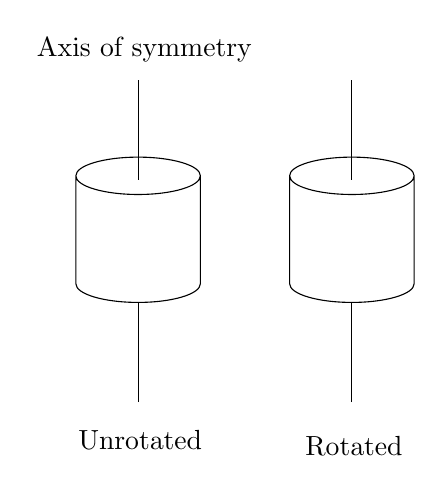
\begin{tikzpicture}[x=0.75pt,y=0.75pt,yscale=-1,xscale=1]
%uncomment if require: \path (0,300); %set diagram left start at 0, and has height of 300

%Shape: Can [id:dp6111663527038986] 
\draw   (154,122) -- (154,174) .. controls (154,178.97) and (140.57,183) .. (124,183) .. controls (107.43,183) and (94,178.97) .. (94,174) -- (94,122) .. controls (94,117.03) and (107.43,113) .. (124,113) .. controls (140.57,113) and (154,117.03) .. (154,122) .. controls (154,126.97) and (140.57,131) .. (124,131) .. controls (107.43,131) and (94,126.97) .. (94,122) ;
%Straight Lines [id:da6016989853853066] 
\draw    (124,124) -- (124,76) ;
%Straight Lines [id:da7742642520386162] 
\draw    (124,231) -- (124,183) ;
%Shape: Can [id:dp6333770541501842] 
\draw   (257,122) -- (257,174) .. controls (257,178.97) and (243.57,183) .. (227,183) .. controls (210.43,183) and (197,178.97) .. (197,174) -- (197,122) .. controls (197,117.03) and (210.43,113) .. (227,113) .. controls (243.57,113) and (257,117.03) .. (257,122) .. controls (257,126.97) and (243.57,131) .. (227,131) .. controls (210.43,131) and (197,126.97) .. (197,122) ;
%Straight Lines [id:da2230680788551479] 
\draw    (227,124) -- (227,76) ;
%Straight Lines [id:da2565843946616415] 
\draw    (227,231) -- (227,183) ;

% Text Node
\draw (125,249) node   [align=left] {Unrotated};
% Text Node
\draw (228,252) node   [align=left] {Rotated};
% Text Node
\draw (127,61) node   [align=left] {Axis of symmetry};


\end{tikzpicture}
    \caption{Symmetry of a cylinder}
    \label{fig:cylinder-rot}
\end{figure}
Mathematically, when we change our position of observation, it is equivalent to using a new, different reference frame and coordinate system, oriented differently from, and/or displaced relative to, the original. So a transformation can be viewed simply as a change of coordinate system, and this is often represented as a shifting from unprimed to primed coordinates. In QFT, \textbf{we will focus on passive transformation interpretation.}

\begin{example}
Consider the function 
\begin{equation}
g\left(x^{1}, x^{2}\right)=\left(x^{2}\right)^{2}
\end{equation}
if we have the following rorational transformation as
$$
\left[\begin{array}{l}
{x^{\prime 1}} \\
{x^{\prime 2}}
\end{array}\right]=\underbrace{\left[\begin{array}{cc}
{\cos \theta} & {\sin \theta} \\
{-\sin \theta} & {\cos \theta}
\end{array}\right]}_T\left[\begin{array}{l}
{x^{1}} \\
{x^{2}}
\end{array}\right]
\quad
\left[\begin{array}{l}
{x^{1}} \\
{x^{2}}
\end{array}\right]=\underbrace{\left[\begin{array}{ll}
{\cos \theta} & {-\sin \theta} \\
{\sin \theta} & {\cos \theta}
\end{array}\right]}_{T^{-1}=T^T}\left[\begin{array}{l}
{x^{\prime1}} \\
{x^{\prime2}}
\end{array}\right]
$$
we can express the function in the primed coordinate as:
$$
g=\left(x^{2}\right)^{2}=\left(x^{\prime 1} \sin \theta+x^{\prime 2} \cos \theta\right)^{2}=\left(x^{\prime 1}\right)^{2} \sin ^{2} \theta+\left(x^{\prime 2}\right)^{2} \cos ^{2} \theta+2 x^{\prime 1} x^{\prime 2} \sin \theta \cos \theta \neq\left(x^{\prime 2}\right)^{2}
$$
The transformed form of $g,$ represented by $g^{\prime}$, has the same value at the same physical point, but it is not the same form in terms of the primed coordinates as $g$ was in terms of the unprimed coordinates. But $f^{\prime},$ the transformed form of $f,$ did have the same form in terms of both sets of coordinates, and thus, we dropped the prime on $f$ on the RHS.

In spite of its non-symmetry under rotation, $g$ is symmetric under a different kind of Fransfort of the firc-symment ander founding $f$ the bynaced relative to the first along transformation, the translation to a coordinate system which is displaced relative to the first along the $x^{1}$ axis, i.e., $x^{1} \rightarrow x^{1}=x^{1}+$ constant $,$ or
$$
\left[\begin{array}{l}
{x^{\prime 1}} \\
{x^{\prime 2}}
\end{array}\right]=\left[\begin{array}{l}
{x^{1}} \\
{x^{2}}
\end{array}\right]+\left[\begin{array}{l}
{K} \\
{0}
\end{array}\right] \quad K=\text { constant }
$$
Substitution yields $g^{\prime}$ have the same form.
\end{example}
\begin{qt}
    From the example above, we can deduce the general rule that if a coordinate is missing in a given function, that function is invariant under a transformation solely in the direction of that coordinate (and also under multiplication of the coordiante by a constant).
\end{qt}
\textbf{\redp{So under any transformation of coordinate axes, the value at a physical point of every possible scalar function is invariant.}}
\subsection{Scalar are invariant, vectors are covariant}
\textbf{The scalar value at the point ( equal to the length of the position vector at that point) is the same in both systems, but the coordinate values are not.} For a 2D position vector in physical space, we have
$$
|x|=\left|x^{i}\right|=\sqrt{\left(x^{1}\right)^{2}+\left(x^{2}\right)^{2}}=\sqrt{\left(x^{\prime1}\right)^{2}+\left(x^{\prime2}\right)^{2}}=\left|x^{\prime i}\right|
$$
It is generally true of every vector $\mathbf{v},$ not just the position vector shown here, that its physical, measurable length (a scalar value) remains unchanged under any coordinate transformation, but its component values change. This is called covariance. Scalar values are invariant under coordinate transformation; vector components are \textbf{covariant}.
\begin{qt}
    General rule: if a function $h$ is not a function of the $j$th coordinate $x^j$, then h is symmetric under the transformation $x^{j} \rightarrow x^{j}+$ constant.
\end{qt}
\section{Symmetry in Classical Mechanics}
Recall that a Galilean transformation is
$$
\left[\begin{array}{c}
{x^{1}} \\
{x^{2}} \\
{x^{3}}
\end{array}\right] \rightarrow\left[\begin{array}{c}
{x^{11}} \\
{x^{\prime 2}} \\
{x^{3}}
\end{array}\right]=\left[\begin{array}{c}
{x^{1}-v^{1} t} \\
{x^{2}-v^{2} t} \\
{x^{3}-v^{3} t}
\end{array}\right]
$$
Newtonian mechanics is invariant under the Galilean transformation. But \textbf{Maxwell's eqs are not invariant under Galilean transformation. Instead, it is invariant under Lorentz transformation}
\begin{qt}
    \begin{equation}
\left[\begin{array}{c}
{x^{0}} \\
{x^{1}} \\
{x^{2}} \\
{x^{3}}
\end{array}\right] \rightarrow\left[\begin{array}{c}
{x^{\prime 0}} \\
{x^{\prime 1}} \\
{x^{\prime 2}} \\
{x^{\prime 3}}
\end{array}\right]=\left[\begin{array}{c}
{\gamma\left(x^{0}-\frac{v}{c} x^{1}\right)} \\
{\gamma\left(x^{1}-\frac{v}{c} x^{0}\right)} \\
{x^{2}} \\
{x^{3}}
\end{array}\right]=\underbrace{\left[\begin{array}{cccc}
{\gamma} & {-\gamma \frac{v}{c}} & {0} & {0} \\
{-\gamma \frac{v}{c}} & {\gamma} & {0} & {0} \\
{0} & {0} & {1} & {0} \\
{0} & {0} & {0} & {1}
\end{array}\right]}_{\Lambda}\left[\begin{array}{c}
{x^{0}} \\
{x^{1}} \\
{x^{2}} \\
{x^{3}}
\end{array}\right]
\label{lorentz-trans}
\end{equation}
where
$$
\gamma=\frac{1}{\sqrt{1-\frac{v^{2}}{c^{2}}}} \quad v=v^{1}
$$
\end{qt}
The index notation for Lorentz transformations is 
\begin{qt}
    \begin{equation}
x^{\prime \mu}=\Lambda^{\mu}{}_{v} x^{v} \quad V^{\prime \mu}\left(x^{\prime \alpha}\right)=\Lambda^{\mu}{}_{v} V^{v}\left(x^{\alpha}\right) \quad T^{\prime \mu v}\left(x^{\prime \alpha}\right)=\Lambda^{\mu}{}_{\delta} \Lambda^{v}{}_{\gamma} T^{\delta \gamma}\left(x^{\alpha}\right)
\end{equation}
Note that $\Lambda^{-1},$ the inverse of $\Lambda,$ can be obtained by taking $\mathbf{v} \rightarrow-\mathbf{v}$ since each coordinate system seems to be going in the opposite direction with respect to the other. $\Lambda^{-1}$ will transform $x^{\prime \mu}$ back into $x^{\mu}$.
\end{qt}
\bluep{Recall that the length of a vector in 3D is unchanged under a coordinate system transformation, 1.e., the length 1s a scalar and thus invariant. The same thing is true in 4D for four-vectors.}
$$
w_{\mu} w^{\mu}=w_{0} w^{0}+w_{1} w^{1}+w_{2} w^{2}+w_{3} w^{3}=w^{0} w^{0}-w^{1} w^{1}-w^{2} w^{2}-w^{3} w^{3}=\text { scalar invariant }
$$
\textbf{and that this is the same for any observer in any inertial coordinate system. This applies to any
vector, be it a position vector like $x^{\mu},$ the differential of position $d x^{\mu},$ the four-velocity $u^{\mu}$, the four potential $A^{\mu}$, the partial derivative $\partial^{\mu}$, or any other}.For instance,
$$
\frac{\partial}{\partial x^{\mu}} \frac{\partial}{\partial x_{\mu}}=\partial_{\mu} \partial^{\mu}=\frac{\partial}{\partial x^{0}} \frac{\partial}{\partial x^{0}}-\frac{\partial}{\partial x^{1}} \frac{\partial}{\partial x^{1}}-\frac{\partial}{\partial x^{2}} \frac{\partial}{\partial x^{2}}-\frac{\partial}{\partial x^{3}} \frac{\partial}{\partial x^{3}}=\text { scalar invariant derivative, }
$$
So if X represents a quantity, we have
$$
\frac{\partial}{\partial x^{\mu}} \frac{\partial}{\partial x_{\mu}}=\frac{\partial}{\partial x^{\prime \mu}} \frac{\partial}{\partial x_{\mu}^{\prime}} \rightarrow \frac{\partial}{\partial x^{\mu}} \frac{\partial}{\partial x_{\mu}} X=\frac{\partial}{\partial x^{\prime\mu}} \frac{\partial}{\partial x_{\mu}^{\prime}} X
$$
\subsection{Poincare transformation}
The most general transformation we could have in spacetime would comprise 1) a 4D translation(translating our coordinate axes in space, time, or both), 2) a rotation in space, and 3) a Lorentz transformation to a frame with different relative velocity. (We ignore reflection.)

The rotation in 3D is the same. It does allow us to rotate our 3D axes, however, so that the relative velocity between our original and transformed systems is along the $x^1$ axes of both. \textbf{This lets us use the Lorentz transformation in its simplest form (\ref{lorentz-trans})}. With this form we state the general transformation between coordinate systems, know as \redp{\textbf{Poincare transformation}} as
\begin{equation}
x^{\mu}=\Lambda_{\nu}^{\mu}\left(x^{\nu}+a^{\nu}\right) \quad a^{\nu}=\mathrm{constant} \text { four vector }
\label{poincare-trans}
\end{equation}

\subsection{Other kinds of symmetry}
Consider the Euler-Lagrange equation for a particle in Newtonian mechanics
$$
\frac{d}{d t}\left(\frac{\partial L}{\partial \dot{x}^{i}}\right)-\frac{\partial L}{\partial x^{i}}=0 \quad L=T-V \quad p_{i}=\frac{\partial L}{\partial \dot{x}^{i}}
$$
If the Lagrangian $L$ is not an explicit function of the spatial coordinate $x^i,$ then $\partial L / \partial x^{i}=0$ on the LHS above. Thus, the time derivative of $p_{i}$ is zero.
$$
\frac{d}{d t}\left(\frac{\partial L}{\partial \dot{x}^{i}}\right)=\frac{d p_{i}}{d t}=0 \quad \text { with } \frac{\partial L}{\partial x^{i}}=0 \quad \text { when } \quad L \neq L\left(x^{i}\right)
$$
Hence $p^i$ is constant and thus, conserved. This makes sense since the only source for spatial dependence in $L$ is the potential energy $V$. If we have no $V$ dependence on $x^i$, then there is no force in the $x^i$ direction, and momentum $p_i$ is constant.\textbf{Note this means the Lagrangian is symmtric.}

\redp{If the Lagrangian is symmetric in a coordinate, then the conjugate momentum for that coordiante is conserved.}

\section{Transformations in QFT}
\subsection{Spinor transformation}
For spinor, we seek a matrix which is four by four in spinor space and which represents what ha~pens to a spmor under a Lorentz transformation and/or a rotation of coordinates. That is, we seek D in
\begin{equation}
\psi^{\prime}\left(x^{\prime \mu}\right)=D \psi\left(x^{\mu}\right) \quad \frac{\text { with spinor indices }}{\text { written out }} \quad \psi_{\alpha}^{\prime}\left(x^{\prime \mu}\right)=D_{\alpha \beta} \psi_{\beta}\left(x^{\mu}\right)
\end{equation}
The spinor transformation under Lorentz and rotation transformation is
\begin{equation}
D=e^{-i(\mathbf{L} \mathbf{\Theta}+\mathbf{M} \mathbf{Q})} \quad L^{k}=-\frac{i}{2} \varepsilon_{i j}^{k} \gamma^{i} \gamma^{j}, \quad \Theta^{k}=\left(\theta^{1}, \theta^{2}, \theta^{3}\right), M^{k}=\frac{i}{2} \gamma^{0} \gamma^{k}, Q^{k}=\left(v^{1}, v^{2}, v^{3}\right)
\end{equation}
where $\Theta^{k}$ represents rotation angles of the primed system with respect to the unprimed system; $Q^k$ is a three vector of the boost velocities; and $\epsilon_{ij}{}^{k}$ is zero unless $i,j,k$ are all different, 1 if $ijk=123,231,312$, and -1 for the others.

Note that in formal mathematical language, the set of all possible Lorentz transformations (all possible v) is known as the Lorentz group. When the Lorentz group acts on the coordinate system, it changes what our spinors look like in the new system and this change is represented by $D$. So, \textbf{$D$ is called a representation of the Lorentz group.} It "represents" that group in spinor space.
\begin{qt}
    $\bar{\psi} \psi=$ world scalar $\quad \bar{\psi} \gamma^{\mu} \psi=$ transforms like four vector.
\end{qt}
\section{Lorentz Symmetry of the Lagrangian Density}
Lagrangian Density is symmetric under Lorentz transformation. We conclude this because of Einstein's postulate that the laws of nature (the field equation here) is invariant in form under Lorentz transformation. The Euler-Lagrange equation for fields, which is another form of the field equation, is a law of nature and must, therefore be invariant in form as well.

\section{Noether's Theorem}
There are other ways the Lagrangian density can be symmetric, for example
\begin{equation}
\phi \rightarrow \phi^{\prime}=\phi e^{-i \alpha}
\label{phase-trans}
\end{equation}
and for free scalar field, we have
$$
\mathcal{L}_{0}^{0}=\partial_{v} \underbrace{\phi^{r+} e^{-i \alpha}}_{\phi^{\dagger}} \partial^{v} \underbrace{\phi^{\prime} e^{i a}}_{\phi}-\mu^{2} \underbrace{\phi^{\prime} e^{-i \alpha}}_{\phi^{\dagger}} \underbrace{\phi^{\prime} e^{i \alpha}}_{\phi}=\mathcal{L}_{0}^{0}\left(\phi^{\prime\dagger}, \phi^{\prime}\right)
$$
\subsection{Internal and external symmetries}
Poincaré transformations (Lorentz plus $4 \mathrm{D}$ translation) and $3 \mathrm{D}$ rotations involve changes $\mathrm{t}$ to physical coordinates $x^{\mu}$ of our external world and are called \textbf{external transformations}.

Transformation like (\ref{phase-trans}) have nothing to do with $x^{\mu}$, but instead function in hidden spaces, behind the scene, like Hilbert or Fock space. They are called \textbf{internal transformation}.
\begin{qt}
   Noether's theorem in words: \textbf{ A symmetry in the Lagrangian density implies an associated quantity is conserved.}
   
   Mathematically:If the Lagrangian density $\mathcal{L}\left(\phi^{r}, \phi^{r}, \mu\right)$ is symmetric in form with respect to a transformation in $\phi^{r}$ which is a function of parameter $\alpha$,i.e., $\phi^{r}\left(x^{\mu}\right) \rightarrow \phi^{r}\left(x^{\mu}, \alpha\right)$ then the four current (using $\left.\phi^{r}\left(x^{\mu}, \alpha\right)\right)$
   \begin{equation}
j^{\mu}\left(\phi^{r}, \phi_{, \nu}^{r}\right)=\frac{\partial \mathcal{L}}{\partial \phi_{, \mu}^{r}} \frac{\partial \phi^{r}}{\partial \alpha} \quad(\text { sum on } r)
\end{equation}
bas zero four-divergence,$\partial_{\mu} j^{\mu}=0$. Thus, its zeroth component $j^0$ integrated over all the space is conserved, as is $q j^{0}$ integrated over all space, where $q$ is a constant.
\end{qt}
\subsection{Apply Noether's theorem to free scalar field}
$$
\frac{\partial \mathcal{L}_{0}^{0}}{\partial \phi_{\mu}}=\frac{\partial}{\partial \phi_{, \mu}}\left(\phi_{, \nu}^{\dagger} \phi^{\nu}-\mu^{2} \phi^{\dagger} \phi\right)=\frac{\partial}{\partial \phi_{\mu}}\left(\phi_{, \mu}^{\dagger} \phi^{\nu}\right)
=\frac{\partial \phi_{, \nu}^{\dagger}}{\partial \phi_{\mu}} \phi^{,\nu}+\phi_{, \nu}^{\dagger} \frac{\partial \phi^{,\nu}}{\partial \phi_{,\mu}}=\phi_{, \nu}^{\dagger} g^{\nu \mu}=\phi^{\dagger, \mu}
$$
$$
\frac{\partial \mathcal{L}_{0}^{0}}{\partial \phi^{\dagger}, \mu}=\frac{\partial}{\partial \phi^{\dagger}, \mu}\left(\phi_{, \nu}^{\dagger} \phi^{\nu}-\mu^{2} \phi^{\dagger} \phi\right)=\frac{\partial}{\partial \phi^{\dagger}}\left(\phi^{\dagger}, \phi^{,\nu}\right)=\frac{\partial \phi^{\dagger}_{, \nu}}{\partial \phi^{\dagger}_{, \mu}} \phi^{,\nu}=\delta_{v}^{\mu} \phi^{, v}=\phi^{,\mu}
$$
and
$$
\begin{array}{l}
{\frac{\partial \phi\left(x^{\eta}, \alpha\right)}{\partial \alpha}=\frac{\partial}{\partial \alpha} \phi\left(x^{\eta}\right) e^{-i \alpha}=-i \phi\left(x^{\eta}\right) e^{-i \alpha}} \\
{\frac{\partial \phi^{\dagger}\left(x^{\eta}, \alpha\right)}{\partial \alpha}=\frac{\partial}{\partial \alpha} \phi^{\dagger}\left(x^{\eta}\right) e^{i \alpha}=i \phi^{\dagger}\left(x^{\eta}\right) e^{i \alpha}}
\end{array}
$$
Using the relation above, we have
$$
j^{\mu}\left(\phi^{r}, \phi^{r}_{,v}\right)=i\left(\phi^{,\mu}\left(x^{\eta}\right) \phi^{\dagger}\left(x^{\eta}\right)-\phi^{\dagger, \mu}\left(x^{\eta}\right) \phi\left(x^{\eta}\right)\right)
$$
This is identical to the scalar four-current.\redp{The expectation value ( expected measurement) of a conserved operator is conserved. If the state measured is in an eigenstate, any measurement at any time will yield the same eigenvalue}.
\section{Symmetry, Gauges, and Gauge theory}
\begin{itemize}
    \item \textbf{Gauge invariance }(or gauge symmetry) is the property of a field theory in which different configurations of the underlying fundamental, but unobservable, field(s) result in identical observable properties.
    \item the unobservable field, often a potential field, is called the\textbf{ gauge field}.
    \item A gauge transformation changes the gauge field from one configuration to another. \redp{Each different configuration of the gauge field is a different gauge.}
    \item A theory have gauge invariance (symmetry) is called a gauge theory.
\end{itemize}
\redp{\textbf{We can also say that a gauge theory is a type of field theory in which the Lagrangian ( density) is invariant under a continuous (not discrete) transformation.}}
\section{A Solved Exercises}
\textbf{Problem 14.} Show that the total (not density) 3-momentum $k^{i}$ for free scalars is conserved. Use our knowledge that the conjugate momentum for $x^{i}$ is $k_{i}$, the total (not density) 3 -momentum (expressed in covariant components), and it is conserved if $L$ is symmetric (invariant) under the coordinate translation transformation $x^{t} \rightarrow x^{1}=x^{t},$ where $\alpha^{t}$ is a constant $3 \square$ vector. Then, show the same result via commutation of the three-momentum operator.

\textbf{Solution}
The Lagrangian density is $\mathcal{L}_{0}^{0}=\phi_{, \mu}^{\dagger} \phi^{\mu}-\mu^{2} \phi^{\dagger} \phi .$ We must integrate this over all volume to get the total Lagrangian $L$. If $k_{i}$ is conserved, then of course, so is $k^{i}$. So, we need to show $L$ is invariant under $x^{i} \rightarrow x^{i}=x^{i}+\alpha^{i}$
$$
\phi=\sum_{\mathbf{k}} \frac{1}{\sqrt{2 V a_{\mathbf{k}}}}\left(a(\mathbf{k}) e^{-i k_{\mu} x^{\mu}}+b^{\dagger}(\mathbf{k}) e^{i k_{\mu} x^{\mu}}\right) \quad \phi^{\dagger}=\sum_{\mathbf{k}} \frac{1}{\sqrt{2 V a_{k}}}\left(b(\mathbf{k}) e^{-i k_{\mu} x^{\mu}}+a^{\dagger}(\mathbf{k}) e^{i k_{\mu} x^{\mu}}\right)
$$
$$
\begin{array}{l}
{\phi_{s}, \mu=\sum_{\mathbf{k}} \frac{i k_{\mu}}{\sqrt{2 V \omega_{\mathbf{k}}}}\left(-a(\mathbf{k}) e^{-i k_{\mu} x^{\mu}}+b^{\dagger}(\mathbf{k}) e^{i k_{\mu} x^{\mu}}\right)} \\
{\phi^{, \mu}=\sum_{\mathbf{k}} \frac{i k^{\mu}}{\sqrt{2 V a_{k}}}\left(-a(\mathbf{k}) e^{-i k_{\mu} x^{\mu}}+b^{\dagger}(\mathbf{k}) e^{i k_{\mu} x^{\mu}}\right)}
\end{array}
$$
$$
\begin{aligned}
\phi^{\dagger}_{z \mu} \phi^{z}=\sum_{\mathbf{k}} \sum_{\mathbf{k}^{*}} \frac{-1}{2 V} \frac{k_{\mu} k^{* \mu}}{\sqrt{\omega_{\mathbf{k}} \omega_{\mathbf{k}^{*}}}}\left(b(\mathbf{k}) a\left(\mathbf{k}^{*}\right) e^{-i k_{A} x^{\mu}} e^{-i k_{A}^{*} x^{\mu}}-b(\mathbf{k}) b^{\dagger}\left(\mathbf{k}^{*}\right) e^{-i k_{\mu} x^{\mu}} e^{i k_{\mu} x^{\mu}}\right.\\
-a^{\dagger}(\mathbf{k}) a\left(\mathbf{k}^{*}\right) e^{i k_{\mu} x^{\mu}} e^{-i k_{\mu} x^{\mu}}+a^{\dagger}(\mathbf{k}) b^{\dagger}\left(\mathbf{k}^{*}\right) e^{i k_{\mu} x^{\mu}} e^{i k_{\mu} x^{\mu}}
\end{aligned}
$$
For $k_{i}=-k^*_i$, we have $$
\left.k_{\mu} k^{* \mu}=\omega_{\mathbf{k}}^{2}+k_{i} k^{*i}=\omega_{\mathbf{k}}^{2}+k_{i}\left(-k^{i}\right)=\omega_{\mathbf{k}}^{2}+k_{i} k_{i}=k_{\mu} k_{\mu}\right.
$$
$$
\int \phi^{\dagger}_{,\mu} \phi^{, \mu} d V=\sum_{k} \frac{-1}{2 \omega_{k}}\left(\begin{array}{c}
{k_{\mu} k_{\mu} e^{-i 2 \omega_{k} t} b(\mathbf{k}) a(-\mathbf{k})-k_{\mu} k^{\mu} b(\mathbf{k}) b^{\dagger}(\mathbf{k})} \\
{-k_{\mu} k^{\mu} a^{\dagger}(\mathbf{k}) a(\mathbf{k})+k_{\mu} k_{\mu} e^{i 2 \omega_{k} t} a^{\dagger}(\mathbf{k}) b^{\dagger}(-\mathbf{k})}
\end{array}\right)
$$
Similarly,
$$
\int \mu^{2} \phi^{\dagger} \phi d V=-\sum_{\mathbf{k}} \frac{\mu^{2}}{2 \omega_{\mathbf{k}}}\left(e^{-i 2 \omega_{\mathbf{k}} t} b(\mathbf{k}) a(-\mathbf{k})+b(\mathbf{k}) b^{\dagger}(\mathbf{k})+a^{\dagger}(\mathbf{k}) a(\mathbf{k})+e^{i 2 \omega_{\mathbf{k}} t} a^{\dagger}(\mathbf{k}) b^{\dagger}(-\mathbf{k})\right)
$$
It is easy to show that, after the transformation the forms of $\int \mu^{2} \phi^{\dagger} \phi d V$ and $\int \phi^{\dagger}_{,\mu} \phi^{, \mu} d V$ will not change, so L is symmetric in some coordinate, then the conjugate momentum of that coordinate is conserved. $k_{i}$, the particle(s) 3 -momentum is the conjugate momentum of $x^{i} .$ Thus, $k_{i}$, is conserved.

Also
$$
H=\sum_{\mathbf{k}} \omega_{\mathbf{k}}\left(N_{a}(\mathbf{k})+N_{b}(\mathbf{k})\right) \quad \mathbf{P}=\sum_{\mathbf{k}} \mathbf{k}\left(N_{a}(\mathbf{k})+N_{b}(\mathbf{k})\right) \rightarrow[H, \mathbf{P}]=0 \quad\left(\begin{array}{ll}
{\text { because all number }} \\
{\text { operators commute }}
\end{array}\right)
$$
Thus $\mathbf{P}$ is conserved for the free Hamiltonian.
\chapter{Interactions: The Underlying Theory}
\section{Interactions in RQM}
\subsection{Maxwell's equation with sources}
If we include the charge density and current density into Maxwell's equation, we have
\begin{equation}
\begin{aligned}
&\nabla \cdot \mathbf{E}=\rho_{charge}\\
&\nabla \times \mathbf{B}-\frac{\partial \mathbf{E}}{\partial t}=\mathbf{j}_{charge}\\
&\nabla \cdot \mathbf{B}=0\\
&\vec{\nabla} \times \mathbf{E}=-\frac{\partial \mathbf{B}}{\partial t}
\end{aligned}
\end{equation}
By introducing the potentials $\Phi$ and $\mathbf{A}$, where 
$$
\mathbf{B}=\nabla \times \mathbf{A}, \quad \mathbf{E}=-\nabla \Phi-\frac{\partial \mathbf{A}}{\partial t}
$$
one gets
\begin{equation}
\begin{aligned}
&-\nabla \frac{\partial \Phi}{\partial t}-\nabla(\nabla \cdot \mathbf{A})=\rho_{charge}\\
&\frac{\partial^{2} \mathbf{A}}{\partial t^{2}}-\nabla^{2} \mathbf{A}+\nabla \frac{\partial \Phi}{\partial t}+\nabla(\nabla\cdot\mathbf{A})=\mathbf{j}_{charge}
\end{aligned}
\end{equation}
Rewrite the equations above in terms of 4-potential and 4-current $-ej^{\mu}$=($\rho_{charge},\mathbf{j}_{charge}$):
\begin{equation}
    \partial^{\alpha}\partial_{\alpha}A^{\mu}(x)-\partial^{\mu}\left(\partial_{\nu}A^{\nu}(x)\right)=-ej^{\mu}(x)
\end{equation}
Using Lorenz gauge condition, we have
\begin{qt}
\begin{equation}
    \partial^{\alpha}\partial_{\alpha}A^{\mu}(x)=-ej^{\mu}
    \label{maxwell-4D-interaction-eqn}
\end{equation}
\end{qt}
\subsection{The classical Lagrangian density for interaction}
The full electromagnetic Lagrangian(density), including interactions, must give rise to (\ref{maxwell-4D-interaction-eqn}) when substituted into the Euler-Lagrange field equation:
$$
\frac{\partial}{\partial x^{v}}\left(\frac{\partial \mathcal{L}}{\partial \phi_{v}^{n}}\right)-\frac{\partial \mathcal{L}}{\partial \phi^{n}}=0, \quad \text { with } \quad \phi^{n}=A_{\mu} ; \mathcal{L}=\mathcal{L}^{e / m}
$$
One can prove that the full electromagnetic field classical Lagrangian is
\begin{qt}
\begin{equation}
\mathcal{L}^{e / m}=\underbrace{-\frac{1}{2}\left(\partial_{v} A_{\mu}(x)\right)\left(\partial^{v} A^{\mu}(x)\right)}_{\mathcal{L}_{0}^{e / m}}+ \underbrace{e j^{\mu}(x) A_{\mu}(x)}_{\mathcal{L}_{1}^{e / m}}
\label{full-electromagnetic-field-classical-lagrangian}
\end{equation}
where "0" and "1" subscripts denote the free and interaction parts, respectively, of the Lagrangian.
\end{qt}
\subsection{Electromagnetic Interactions in RQM}
Relations (\ref{maxwell-4D-interaction-eqn}) and (\ref{full-electromagnetic-field-classical-lagrangian}) hold for classical electromagnetism where $-ej^{\mu}$ is the classical electric charge 4-current. \textbf{In quantization, we assume the quantum form of the Lagrangian (density or total) is the same as the classical, and thus, so would be the resulting wave equation.} In RQM, we would then consider $A^{\mu}$ to represent the quantum photon state (ket, wave function). Thus, (\ref{full-electromagnetic-field-classical-lagrangian}) represents the RQM electromagnetic Lagrangian. But then, \bluep{how should one interpret $-ej^{\mu}$?} In Chap.3, we saw that the probability 4-current for an electron in RQM, where $\psi_{state}$ represents the electron wave function state, is
$$
j^{\mu}=(\rho, \mathbf{j})=\bar{\psi}_{\text {state}} \gamma^{\mu} \psi_{\text {state}} \quad \text { where } \partial_{\mu} j^{\mu}=0
$$
\redp{It seems natural to assume charge density varies directly with probability density.} Thus, we can assume
\begin{equation}
-e j^{\mu}=-e \bar{\psi}_{\text {state}} \gamma^{\mu} \psi_{\text {state}}
\label{electron-4-current-state}
\end{equation}
where the total charge of the electron would be
$$
-e \int j^{0} d^{3} x=-e
$$
Using (\ref{maxwell-4D-interaction-eqn}),(\ref{full-electromagnetic-field-classical-lagrangian}), and(\ref{electron-4-current-state}), we can then represent the \textbf{\redp{RQM interaction wave equation for a photon}} as
\begin{equation}
\partial^{\alpha} \partial_{\alpha} A_{\text {stale}}^{\mu}=-e \bar{\psi}_{\text {state}} \gamma^{\mu} \psi_{\text {state}}
\label{RQM-photon-interaction-wave-eqn}
\end{equation}
with the corresponding \textbf{\redp{RQM e/m interaction Lagrangian for a photon}} as
\begin{equation}
\mathcal{L}^{e / m}=\underbrace{-\frac{1}{2}\left(\partial_{v} A_{\mu,state}\right)\left(\partial^{v} A_{\text {state }}^{\mu}\right)}_{\mathcal{L}_0^{e/m}}+\underbrace{e \bar{\psi}_{\text {state}} \gamma^{\mu} \psi_{\text {state}} A_{\mu,state}}_{\mathcal{L}_I^{e/m}}
\label{RQM-em-interaction Lagrangian-for-photon}
\end{equation}
\redp{\textbf{(\ref{RQM-photon-interaction-wave-eqn}) governs the behavior of a photon ($A^{\mu}_{state}$) in the presence of an electron ($\psi_{state}$)}}.
\subsection{The electromagnetic interaction Dirac equation}
We now develop the full Dirac equation describing the electron interacting with a photon. To this end, consider that $\mathcal{L}_{0}^{e / m}$ of (\ref{RQM-em-interaction Lagrangian-for-photon}) represents the free photon part of the full e/m Lagrangian. If we assume $\mathcal{L}_{1}^{e / m}$ represents the e/m interaction part for both the photon and the electron, then \textbf{\redp{we need only add the free electron contribution to (\ref{RQM-em-interaction Lagrangian-for-photon}) to get a Lagrangian containing all terms relevant to photons, electrons, and interactions between them.}} Since from Chap 3
$$
\mathcal{L}_{0}^{1 / 2}=\bar{\psi}_{\text {state}}\left(i \gamma^{\mu} \partial_{\mu}-m\right) \psi_{\text {state}}
$$
Thus, the \textbf{full e/m Lagrangian} is
\begin{equation}
\mathcal{L}^{1 / 2,1}=\underbrace{-\frac{1}{2}\left(\partial_{v} A_{\mu,state}\right)\left(\partial^{v} A_{\text {state}}^{\mu}\right)}_{\mathcal{L}_{0}^{1}=\mathcal{L}_{0}^{e / m}}+\underbrace{\bar{\psi}_{\text {state}}\left(i \gamma^{\mu} \partial_{\mu}-m\right) \psi_{\text {state}}}_{\mathcal{L}_{0}^{1 / 2}}+\underbrace{e \bar{\psi}_{\text {state}} \gamma^{\mu} \psi_{\text {state}} A_{\mu,state}}_{\mathcal{L}_{1}^{1 / 2,1}=\mathcal{L}_{1}^{e/m}}
\label{full-e/m-lagrangian}
\end{equation}
To find the interaction form of the Dirac equation, we use (\ref{full-e/m-lagrangian}) in Euler-Lagrange equation with $\phi^{n=1}=\bar{\psi}$. The result is
\begin{qt}
\begin{equation}
\left(i \gamma^{\mu} \partial_{\mu}-m\right) \psi_{\text {state }}=-e \gamma^{\mu} \psi_{\text {state }} A_{\mu,state}
\label{full-Dirac-eqn}
\end{equation}
As an aside, using (\ref{full-e/m-lagrangian}) with $\phi^{n=2}=\psi$ results in the adjoint full Dirac equation.
\end{qt}

\begin{mybox}
A this point, some might be concerned that we have used the Lagrangian density methodology, which is normally reserved for quantum and classical fields, to develop the full Dirac equation for quantum states (corresponding to particles, not fields).One would expect to use the
total Lagrangian L (integration of $\mathcal{L}$ over all space) instead of $\mathcal{L}$, since (\ref{full-Dirac-eqn}) is a wave equation for interacting states, not fields.

However, even in the context of $1^{\text {st }}$ (particle) and $2^{\text {nd }}$ (field) quantization as we have come to understand them, the issue is not such a big one. This is because we did not employ commutation relations for fields $A^{\mu}$ and $\psi,$ analogous to Poisson bracket relations, in the above development, It is the adth $^{\mu} A^{\mu}$ and $\psi,$ analogous to Poisson bracket relations, in the above development, \textbf{it is the adoption of commutation relations for those fields that turns them into creation and destruction operators quantum mechanically.} We did not do that, so $A^{\mu}$ and $\psi$ remain as states, not quantum fields, in the above treatment. Of course, for RQM, we would still have commutation relations for dynamical variable gnerators, such as $p_{x}$ and $X_{1}$, though we would not have them for $A^{\mu}$ and $\psi$
\end{mybox}
\section{Interactions in QFT}
Our interacting spinor field and photon wave equations in the Heisenberg picture should simply be the following for fields,
\begin{equation}
\partial^{\alpha} \partial_{\alpha} A^{\mu}=-e \bar{\psi} \gamma^{\mu} \psi
\label{fields-interaction-wave-eqn-1}
\end{equation}
\begin{equation}
\left(i \gamma^{\mu} \partial_{\mu}-m\right) \psi=-e \gamma^{\mu} A_{\mu} \psi
\label{fields-interaction-wave-eqn-2}
\end{equation}
where the order of $\psi$ and $A_{\mu}$ in the equations above is unimportant, even though they are operators, since \redp{different type fields commute}. The associated Lagrangian for the $\psi$ and $A^{\mu}$ operator fields is
\begin{equation}
\mathcal{L}^{1 / 2,1}=\underbrace{-\frac{1}{2}\left(\partial_{v} A_{\mu}\right)\left(\partial^{v} A^{\mu}\right)}_{\mathcal{L}_{0}^{1}}+\underbrace{\bar{\psi}\left(i \gamma^{a} \partial_{\alpha}-m\right) \psi}_{\mathcal{L}_0^{1/2}}+\underbrace{e \bar{\psi} \gamma^{\mu} A_{\mu} \psi}_{\mathcal{L}_{I}^{1 / 2,1}}
\end{equation}

Modern day computers can help in providing numerical solutions to these equations, but early researchers in QFT did not have such things. Also, the route those researchers did take provides considerable insight into the inner workings of the theory. That route, for the QFT e/m interaction theory known as \textbf{quantum electrodynamics (QED)}, was forged in large part by Richard Feynman, Freeman Dyson, Julian Schwinger, and Sin-Itiro Tomonaga. It involves two things,
\begin{itemize}
    \item perturbation theory, and
    \item a trick known as the Interaction picture
\end{itemize}
\begin{qt}
The expectation value for any quantum field, including spinor and vector fields, is zero.
\end{qt}

\section{Interaction Picture}
It turns out that a third picture, the Interaction Picture (I.P.) is easier to use for interactions in
QFT. For one reason, it facilitates use of perturbation theory in place of trying to solve the coupled, non-linear, partial differential equations (\ref{fields-interaction-wave-eqn-1}) and (\ref{fields-interaction-wave-eqn-2}).

Additionally, the LP. allows us to analyze interacting fields using all the results of our free QFT development.

\underline{Breaking the Hamiltonian into Free and Interaction Parts}
The Hamiltonian (total, not density) for e/m interactions in the (Schrödinger Picture) S.P. can be expressed, from the Lagrangian density (\ref{full-e/m-lagrangian}) and the Legendre transformation, as (with $\phi^{r}$ generically representing any quantum field)
\begin{equation}
\underbrace{H^{S}}_{H}=\underbrace{H^{1 / 2,1}}_{\text {just e/m }}=\underbrace{\int\left(\pi_{r} \dot{\phi}^{r}-\mathcal{L}_{0}^{1}-\mathcal{L}_{0}^{1 / 2}\right) d^{3} x}_{H_{0}^{S}=H_{0}(\text { free part })}-\underbrace{\int \mathcal{L}_{I}^{1 / 2,1} d^{3} x}_{H_{I}^{S}(\text { interaction part })}
\end{equation}
Thus,$H=H_{0}+H_{I}^{S}$. Note, for future reference, that for all cases  $\mathcal{H}_{I}=-\mathcal{L}_{I}$ and $ H_{I}=-L_{I}$.

\underline{Using only the free part of the Hamiltonian to transform to the interaction picture}

The transformation from the S.P. to the I.P. is
\begin{equation}
    U_{0}=e^{-i H_{0} t}
\end{equation}
where $U_0$ is a unitary operator, where
\begin{equation}
U_{0}^{\dagger}|\Psi\rangle_{S}=|\Psi\rangle_{I}
\end{equation}
and where subscripts "S" and "I" on generic states $|\Psi\rangle$ indicate the S.P. and I.P, respectively. For operators, where superscripts "S" and "I" represent the S.P. and I.P., respectively,
\begin{equation}
U_{0}^{\dagger} \mathcal{O}^{S} U_{0}=\mathcal{O}^{I}
\end{equation}

\underline{Parts of the Hamiltonian expressed in the I.P.}

For the free part of the Hamiltonian operator $H_{0}=H_{0}^{S},$ we see that
\begin{equation}
H_{0}^{I}=U_{0}^{\dagger} H_{0}^{S} U_{0}=U_{0}^{\dagger} H_{0} U_{0}=e^{i H_{0} t} H_{0} e^{-i H_{0} t}=H_{0} e^{i H_{0} t} e^{-i H_{0} t}=H_{0}
\end{equation}
because $H_{0}$ commutes with itself. Thus,
\begin{equation}
H_{0}=H_{0}^{S}=H_{0}^{I}
\end{equation}
\bluep{this equality generally does not hold for the interaction part:}
$$
H_{I}^{I}=U_{0}^{\dagger} H_{I}^{S} U_{0} \neq H_{I}^{S}
$$
and thus, we will represent the interaction picture Hamiltonian as
\begin{equation}
H^{I}=H_{0}+H_{I}^{I}
\end{equation}
\subsection{Equations of Motion in the I.P.}
$$
\frac{d \mathcal{O}^{l}}{d t}=\frac{d}{d t}\left(U_{0}^{+} \mathcal{O}^{s} U_{0}\right)=\frac{d U_{0}^{\dagger}}{d t} \mathcal{O}^{s} U_{0}+\underbrace{U_{0}^{\dagger} \frac{\partial \mathcal{O}^{S}}{\partial t} U_{0}}_{\text {defined }=\frac{\partial \mathcal{O}^{I}}{\partial t}}+U_{0}^{\dagger} \mathcal{O}^{s} \frac{d U_{0}}{d t}=
$$
$$
\frac{d e^{i H_{0} t}}{d t} \mathcal{O}^{S} e^{-i H_{0} t}+e^{i H_{0} t} \mathcal{O}^{S} \frac{d e^{-i H_{0} t}}{d t}+\frac{\partial \mathcal{O}^{I}}{\partial t}=i H_{0} \underbrace{e^{i H_{0} t} \mathcal{O}^{S} e^{-i H_{0} t}}_{\mathcal{O}^{I}}-\underbrace{e^{i H_{0} t} \mathcal{O}^{S} e^{-i H_{0} t}}_{\mathcal{O}^{I}} i H_{0}+\frac{\partial \mathcal{O}^{I}}{\partial t}
$$
or
\begin{qt}
\begin{equation}
\frac{d \mathcal{O}^{I}}{d t}=-i\left[\mathcal{O}^{I}, H_{0}\right]+\frac{\partial \mathcal{O}^{I}}{\partial t}
\label{IP-operator-time-derivative}
\end{equation}
\end{qt}
where the last term is zero in this note, because we only deal with operators for which $\partial \mathcal{O}^{S} / \partial t=0$. \redp{Thus, the equation of motion for operators in the I.P. depends only on the free part of the Hamiltonian.}

The \underline{I.P. equation of motion for states is}
\begin{equation}
i \frac{d}{d t}|\Psi\rangle_{I}=H_{I}^{I}|\Psi\rangle_{I}
\label{IP-eq-of-motion-state}
\end{equation}
\redp{and hence, the equation of motion for states in the I.P. depends only on the interaction part of the Hamiltonian.}

\underline{The I.P. equation of motion for expectation values is}
\begin{equation}
\frac{d \overline{\mathcal{O}}}{d t}={}_{I}\left\langle\Psi\left|\left(-i\left[\mathcal{O}^{I}, H^{I}\right]+\frac{\partial \mathcal{O}^{I}}{\partial t}\right)\right| \Psi\right\rangle_{I}
\end{equation}
\begin{mybox}
Note that (\ref{IP-operator-time-derivative}) has the same form as the operator equation of motion in the H.P., except that we have $H_0$ in the I.P. and H in the H.P.\textbf{ Hence, we can teke all results we obtained for operator behavior in the H.P. free field and use them in the I.P. for interacting fields.}

For field operators such as $\mathcal{O}^{l}=\phi,\psi, \text { or } A^{\mu})$, (\ref{IP-operator-time-derivative}) has identical form to the H.P. equation of motion for fields where $H=H_0$. Thus (\ref{IP-operator-time-derivative}) reduces to the Klein-Gordon equation for scalars, the free Dirac equation for spinor fields, and the free Maxwell equation for photons. \textbf{Quantum fields in the I.P. behave just like the free quantum fields}
\end{mybox}
\subsection{Visualizing states in the I.P.}
Consider a single  particle scalar plane wave state expressed in the coordinate basis. In the S.P., it looks like, where K is a normalization factor and sub/superscript meaning should be obvious,
$$
|\phi\rangle_{S}=\phi_{\text {state }}^{S}=K e^{-i E t+i \mathbf{k} \cdot \mathbf{x}}=K e^{-i E_{0} t-i E_{I} t+i \mathbf{k} \cdot \mathbf{x}}
$$
Note that $E_{t}$ is a number, and thus is the same in any picture. Transform the state to the I.P.,
$$
U_{0}^{\dagger}|\phi\rangle_{S}=e^{i H_{0} t} \phi_{S, \text { state }}=K e^{i H_{0} t} e^{-i E_{0} t-i E_{I} t+i k \cdot x}=K e^{i E_{0} t} e^{-i E_{0} t-i E_{I} t+i \mathbf{k} \cdot \mathbf{x}}=K e^{-i E_{I} t+i \mathbf{k} \cdot \mathbf{x}}
$$
So we see that \redp{the state in the I.P. varies in time only with the interaction energy}. The operator $U_{0}^{\dagger}$ takes out the $H_{0}$ dependence of the ket.

In the I.P.
\begin{itemize}
    \item the state equation of motion depends on only the interaction Hamiltonian $H_I^I$, \item operator equations of motion depend on only the free Hamiltonian $H_{0},$ thus, importantly, 
    \item the operator equations of motion in the I.P. are the same as the operator equations of motion in the H.P. for free fields (i.e., for $\left.H^{H}=H_{0} \text { with } H_{I}^{H}=0\right),$ so all operator relations derived for free field are valid in I.P.
    \item meaning the free field case Klein-Gordon, Dirac, and Maxwell equations (of motion) from the H.P. are the same as those in the interacting case in the I.P., and so
    \item quantum fields $\phi, \psi,$ and $A^{\mu}$ in the L.P. (the solutions to the field equations of motion) are the same as the free quantum fields solutions in the H.P.
\end{itemize}
So in the I.P. \redp{We only need to solve the state equation of motion(\ref{IP-eq-of-motion-state}).}
\section{S matrix}
\redp{Each $S_{f i}$ of $S$ Matrix is the transition amplitude between an initial eigenstate and a final eigenstate, $S_{f i}^{2}$ is probability of transition from initial eigenstate $|i\rangle$ to final eigenstate $|f\rangle$}. For example
\begin{center}
    $S_{21}^{\dagger} S_{21}=\left|S_{21}\right|^{2}=$ probability of 1 st eigenstate transitioning to $2 \mathrm{nd}$
\end{center}
$S_{fi}$ is a transition amplitude for a particular reaction. That is, for the operator $S_{oper,fi}$
$$
S_{fi}=\left\langle f\left|S_{\text {oper}, fi}\right| i\right\rangle
$$
\begin{equation}
\left.S_{\text {oper}, f i}|i\rangle= S_{f i}|f\rangle \quad \text { (no sum on } i \text { or } f\right)
\end{equation}
and
\begin{equation}
\sum_{f}\left|S_{fi}\right|^{2}=1
\end{equation}
in general
\begin{qt}
\begin{equation}
S_{f i}=\left\langle f\left|S_{o p e r}\right| i\right\rangle
\end{equation}
\end{qt}
\section{Finding the S operator}
We can find the $S_{\text {oper }}$ from the state equation of motion, the only thing we haven't already solved for in the I.P. formulation. In the I.P., our state equation of motion, where $\mathbf{\Psi}$ ) represents a generic state (multiparticle typically), is
$$
i \frac{d}{d t}|\Psi(t)\rangle_{I}=H_{I}^{I}|\Psi(t)\rangle_{I}
$$
Let
\begin{equation}
|F\rangle=\sum_{f} S_{f i}|f\rangle=\left|\Psi\left(t_{f}\right)\right\rangle_{I}=S_{o p e r}\left(t_{f}, t_{i}\right)\left|\Psi\left(t_{i}\right)\right\rangle_{I}=S_{o p e r}\left(t_{f}, t_{i}\right)|i\rangle
\end{equation}
Taking our final time $t_f$ as time $t$ in the eqn. of motion, we have
\begin{equation}
|\Psi(t)\rangle_{I}=S_{\text {oper}}\left(t, t_{i}\right)\left|\Psi\left(t_{i}\right)\right\rangle_{I}
\end{equation}
Using the equation  above in the equation of motion for state yields
\begin{equation}
i \frac{d}{d t}\left(S_{o p e r}\left|\Psi\left(t_{i}\right)\right\rangle_{I}\right)=H_{l}^{I}\left(S_{o p e r}\left|\Psi\left(t_{i}\right)\right\rangle_{I}\right)
\end{equation}
This becomes
\begin{equation}
i \frac{d S_{\text {oper }}}{d t}\left|\Psi\left(t_{i}\right)\right\rangle_{I}+i S_{\text {oper }}\underbrace{ \frac{d}{d t}\left|\Psi\left(t_{i}\right)\right\rangle_{I}}_{=0\text{ as indep. of }t_f}=H_{I}^{I} S_{\text {oper }}\left|\Psi\left(t_{i}\right)\right\rangle_{I}
\end{equation}
\begin{qt}
and thus the differential equation for $S_{oper}$
\begin{equation}
i \frac{d S_{\text {oper}}}{d t}=H_{I}^{I} S_{\text {oper}}
\end{equation}
This has the solution
\begin{equation}
S_{\text {oper}}=e^{-i \int_{t_{i}}^{t_{f}} H_{I}^{I} d t}=e^{-i \int_{t_{i}}^{I f} \int_{V} \mathcal{H}_{I}^{I} d^{4} x}
\end{equation}
In infinite volume and time frame,
\begin{equation}
S=S_{\text {oper }}\left(V\rightarrow\infty t_{f} \rightarrow \infty, t_{i} \rightarrow-\infty\right)=e^{-i \int_{-\infty}^{\infty} \mathcal{H}_{I}^{I} d^{4} x}
\label{S-oper}
\end{equation}
\end{qt}
\begin{mybox}
In Fock space where every eigenstate can be visualized as a separate axis in an infinite dimensional space, the $S_{oper}$ can be visualized as a sort of abstract "rotation" in that space. \textbf{The initial state vector $|i\rangle$ is "rotated" by the $S_{oper}$ into a new vector with components along the eigenstate basis axes.}
\end{mybox}
\section{Expanding S operator}
$S_{oper}$ can be expanded (in a Taylor series like $e^{x}=1+x+x^{2} / 2 !+x^{3} / 3 !+\ldots$ ) as
$$
S_{o p e r}\left(t_{f}, t_{i}\right)=e^{-i \int_{t_{i}}^{t_{f}} H_{I}^{I}(t) d t}=\sum_{n=0}^{\infty} \frac{(-i)^{n}}{n !} \int_{t_{i}}^{t_{f}} \dots \int_{t_{i}}^{t_{f}} T\left\{H_{I}^{I}\left(t_{1}\right) H_{I}^{I}\left(t_{2}\right) \dots H_{I}^{I}\left(t_{n}\right)\right\} d t_{1} d t_{2} \dots d t_{n}
$$
If the $H^{I}$ above were numeric functions of time, it wouldn't really matter what order, with respect to the $t_{n}$, we carry out the integrations above. However, since they are comprised of operators that act on a ket state to their right, we have to be sure that at each point in the integration, the time-wise earliest operators are acting first.

This means that at each point in the $n$ dimensional space each axis is a different $t_{n}$, the $H_{I}^{I}$ dependent on the earliest time of the $t_{n}$ should act first, the $H_{I}^{I}$ dependent on the next earliest of the $t_{n}$ should act next. \textbf{The e order of the integrand operators is rearranged as we integrate over all $t_n$ dimensions, such taht the operator are time ordered at every point ($t_1,t_2,t_3,...$)}

Taking our integration limits to infinity in both space and time into the time ordered infinite spacetime $S_{\text {oper }},$ i.e., the \textbf{Dyson expansion of the S operator},
\begin{qt}
\begin{equation}
S=\sum_{n=0}^{\infty} \frac{(-i)^{n}}{n !} \int_{-\infty}^{\infty} \ldots . \int_{-\infty}^{\infty} T\left\{\mathcal{H}_{I}^{I}\left(t_{1}\right) \mathcal{H}_{I}^{I}\left(t_{2}\right) \ldots \mathcal{H}_{I}^{I}\left(t_{n}\right)\right\} d^{4} x_{1} d^{4} x_{2} \ldots d^{4} x_{n}
\end{equation}
Also note the symbols we can use for the terms above as
$$
S=\underbrace{I}_{S^{(0)}}\underbrace{-i \int_{-\infty}^{\infty} \mathcal{H}_{I}^{I}\left(x_{1}\right) d^{4} x_{1}}_{S^{(1)}}\underbrace{-\frac{1}{2!} \int_{-\infty}^{\infty} \int_{-\infty}^{\infty} T\left\{\mathcal{H}_{I}^{I}\left(x_{1}\right) \mathcal{H}_{I}^{I}\left(x_{2}\right)\right\} d^{4} x_{1} d^{4} x_{2}}_{S^{(2)}}+...=\sum_{n=0}^{\infty} S^{(n)}
$$
\end{qt}

\section{Wick's Theorem Applied to Dyson Expansion}
Time ordering is cumbersome to handle, because \textbf{we can't keep the same order of operators throughout the integration over time}. Fortunately, we can convert $S$ into non-time ordered form, where the order of operators does not change during integration, via a handy theorem developed by Gian-Carlo Wick.

\redp{Wick's theorem converts time ordered products of operators into normal ordered t products of operators and some things called "contractions".}
\begin{qt}
For generic fields $A$ and $B$ (either of which could be $\phi, \psi, A^{\mu}, \phi,$ etc) where
$$
A=\underbrace{A^{+}}_{\text {destruc }}+\underbrace{A^{-}}_{\text {creation }}=A^{d}+A^{c}
$$
$$
B=\underbrace{B^{+}}_{\text {destruc }}+\underbrace{B^{-}}_{\text {creation }}=B^{d}+B^{c}
$$
A contraction is defined as (note the under bracket symbol)
\begin{equation}
\underbracket{A\left(x_{1}\right) B}\left(x_{2}\right)=\left[A_{1}^{+}\left(x_{1}\right), B^{-}\left(x_{2}\right)\right]_{\mp}=\left[A^{d}\left(x_{1}\right), B^{c}\left(x_{2}\right)\right]_{\mp} \quad \text { if } t_{2}<t_{1}
\end{equation}
\begin{equation}
=\pm\left[B^{+}\left(x_{2}\right), A^{-} \left(x_{1}\right)\right]_{\mp}=\pm\left[B^{d}\left(x_{2}\right), A^{c}\left(x_{1}\right)\right]_{\mp} \quad \text { if } t_{1}<t_{2}
\label{contraction}
\end{equation}
In these two cases, we have two sets of time+location coordinates $(t_1,x_1)$ and $(t_2,x_2)$. The plus sign subscript implies anti-commutation, which is used \textbf{is both A and B are fermions.}$\pm$ in front of the relations on the 2 nd row takes a "+" sign for commutation, "-" for anti-commutation. \redp{All commutators/anti-commutators are zero unless $A=\phi$ and $B=\phi^{\dagger}$, or $A=\psi$ and $B=\bar{\psi}$.}
\end{qt}
Note that (\ref{contraction}) has the same form as the Feynmann propagator. Thus, whenever a contraction of scalar field is non-zero, it is a scalar Feynmann propagator. Similar results hold for Spinor and photon fields. Thus, \bluep{special cases of contractions (the only non-zero cases) are}
\begin{equation}
    \underbracket{\phi\left(x_{1}\right) \phi^{\dagger}}\left(x_{2}\right)=\underbracket{\phi^{\dagger}\left(x_{2}\right) \phi}\left(x_{1}\right)=i \Delta_{F}\left(x_{1}-x_{2}\right)
    \label{contraction-scalar-field}
\end{equation}

Remember, the propagator is a number because of the commutation relations like $[a(k),a^{\dagger}(k)]=[b(k),b^{\dagger}(k)]=1$.
\begin{equation}
    \underbracket{\psi_{\alpha}\left(x_{1}\right) \bar{\psi}}_{\beta}\left(x_{2}\right)=-\underbracket{\bar{\psi}_{\beta}\left(x_{2}\right) \psi}_{ }\left(x_{1}\right)=i S_{F \alpha \beta}\left(x_{1}-x_{2}\right)
    \label{contraction-spinor-field}
\end{equation}

\begin{equation}
    \underbracket{A^{\mu}\left(x_{1}\right) A}^{\nu}\left(x_{2}\right)=i D_{F}^{\mu \nu}\left(x_{1}-x_{2}\right)
    \label{contraction-em-field}
\end{equation}

\subsection{Review of normal ordering}
Normal ordering consists of placing construction operators to the right-hand side inside a given term.
\begin{center}
    $N(A B C D \ldots)=$ all destruction operators placed to right of all creation operators.
\end{center}
As part of our definition of normal ordering, note that the \textbf{switching places of two adjacent fermionic fields gives rise to a sign change}. This can be justified, in part, because fermionic fields obey anti-commutation relations. For example $^{1},$ given $[C, D]_{+}=0, C D=-D C$
\begin{qt}
Normal ordering of terms including contractions:

For B a destruction operator
\begin{equation}
N\left\{\underbracket{A\left(x_{1}\right) B^{d}\left(x_{2}\right) C}\left(x_{3}\right)\right\}=\pm \underbracket{A\left(x_{1}\right) C}\left(x_{3}\right) B^{d}\left(x_{2}\right)
\end{equation}
where minus sign for C and $B^{d}$ both fermionic. And for B a creation operator
\begin{equation}
N\left\{\underbracket{A\left(x_{1}\right) B^{c}\left(x_{2}\right) C}\left(x_{3}\right)\right\}=\pm B^{c}\left(x_{2}\right) \underbracket{A\left(x_{1}\right) C}\left(x_{3}\right)
\end{equation}
\end{qt}
\begin{mybox}
We will henceforth use subscripts in place of parenthesis arguments for fields, i.e.,
$$
A\left(x_{1}\right) \rightarrow A_{x_{1}} \quad A\left(x_{1}\right) B\left(x_{1}\right) C\left(x_{1}\right) \rightarrow(A B C)_{x_{1}}
$$
$$
\psi\left(x_{1}\right) \gamma^{\mu} A_{\mu}\left(x_{1}\right) \bar{\psi}\left(x_{1}\right) \rightarrow\left(\psi \gamma^{\mu} A_{\mu} \bar{\psi}\right)_{x_{1}}
$$
\end{mybox}
\subsection{Wick's theorem}
We only state Wick's theorem here and leave the justification to other textbook. The theorem turns a time ordered product into a series of normal ordered terms and contractions, which, as we noted, helps us in calculating interaction probabilities, because we can keep the operators in the same order as we integrate over time.
\begin{qt}
$$
T\left\{(A B \ldots)_{x_{1}} \ldots \ldots(A B \ldots)_{x_{n}}\right\}=N\left\{(A B \ldots)_{x_{1}} \ldots \ldots .(A B \ldots)_{x_{n}}\right\}
$$
$$
+N\left\{(\underbracket{A B . .) x_{1}(A} B .) x_{2} \cdots\right\}+N\left\{(\underbracket{A B . .) x_{1}(A B} .) x_{2} \cdots\right\}+\dots
$$
\begin{equation}
    +N\left\{(\overunderbraces{&\br{2}{A-A-contraction}}{&A&B C...) x_{1}(&AB}{&&\br{2}{B-B-contraction}}C...) x_{2} \cdots\right\}+N\left\{(\overunderbraces{&\br{2}{A-A-contraction}}{&A&BC.. .) x_{1}(&ABC}{&&\br{2}{B-C-contraction}}...) x_{2} \cdots\right\}+etc
\label{wick-theorem}
\end{equation}
Note that there are no contractions between operators operating-at the same time. We say there
are no "equal times contractions" in Wick's theorem. \redp{Equal-time contractions don't play a role in Wick's theorem for QED}.
\end{qt}

\section{Wick's Theorem in Words}
To get Wick's theorem, we start with a series of operator fields, operating in arbitrary order and
set it equal to itself, i.e., $A_{1} B_{2} C_{3} D_{4} \ldots=A_{1} B_{2} C_{3} D_{4} \ldots$

On the LHS, we then re-arrange operator fields using commutation/ant-commutation relations such that earlier times are to the right of later times. We herein use the symbol $T_{c}$ to represent this re-ordering procedure.  The final result of the LHS equals the original LHS expression, since at each, we simply substituted equivalent relations for the original pair of adjacent operators.

On the RHS, we re-arrange operator fields using commutation/anti-commutation relations such that destruction are all to the right of creation operators. We herein use the symbol $N_{c}$ to represent this re-ordering procedure. The final result of the RHS equals the original RHS expression.

The final result of these operations is the same as employing Wick's theorem.

\section{Comment on Normal Ordering of the Hamiltonian Density}
Non-zero commulators (anti-commulators) values are very small, $\approx0$ at macroscopic scales. So from human perspective, all fields effectively commute(anti-commute). So $\mathcal{H}$ could be normal ordered at microscale, but our classical theory formulation would be blind to it \& have evolved in non-normal ordered from.
\chapter{QED: Quantum Field Interaction Theory Applied to EM}
\section{Dyson-Wick's Expansion/or QED Hamiltonian Density}
The Dyson expansion of the S operator is
\begin{equation}
S=I-i \int_{-\infty}^{\infty} \mathcal{H}_{I}^{I}\left(x_{1}\right) d^{4} x_{1}-\frac{1}{2 !} \int_{-\infty}^{\infty} T\left\{\mathcal{H}_{I}^{I}\left(x_{1}\right) \mathcal{H}_{l}^{I}\left(x_{2}\right)\right\} d^{4} x_{1} d^{4} x_{2}+\ldots .
\label{dyson-wick-expansion}
\end{equation}
For the interaction Hamiltonian density in (\ref{dyson-wick-expansion}) we use the relation discovered to work for RQM, because we have learned that Hamiltonians for RQM expressed in the Schrödinger Picture, as a rule, take the same form for QFT expressed in the Heisenberg Picture. We are working in the Interaction Picture, for which operators (such as the Hamiltonian density) take the same form in the I.P. as in the H.P. So, for electromagnetic interactions between electrons, positrons, and photons, the quantum Hamiltonian density takes the form, where, $A_{\mu}\gamma^{\mu}=\cancel{A}$
\begin{equation}
\mathcal{H}_{I}^{I}=-\mathcal{L}_{I}^{I}=-e \bar{\psi} A_{\mu} \gamma^{\mu} \psi=-e \bar{\psi} \cancel{A} \psi=-e\left(\bar{\psi}^{+}+\bar{\psi}^{-}\right)\left(A^{+}+\bar{A}^{-}\right)\left(\psi^{+}+\psi^{-}\right)
\end{equation}
and
\begin{equation}
S=\underbrace{I}_{S^{(0)}} + \underbrace{i e \int_{-\infty}^{\infty}(\bar{\psi} \cancel{A} \psi)_{x_{1}} d^{4} x_{1}}_{S^{(1)}}-\underbrace{\frac{1}{2 !} e^{2} \int_{-\infty}^{\infty} \int_{-\infty}^{\infty} T\left\{(\bar{\psi} \cancel{A} \psi)_{x_{1}}(\bar{\psi} \cancel{A} \psi)_{x_{2}}\right\} d^{4} x_{1} d^{4} x_{2}}_{S^{(2)}}+\dots
\label{explicit-S}
\end{equation}
\bluep{We can approximate (\ref{explicit-S}) by taking only the first few terms.} In this chapter, we only deal with $S^{(0)},S^{(1)},S^{(2)}$.

The second term in (\ref{explicit-S}) has factors operating all at the same time $t_1$, and so can be considered time ordered. Wick's theorem for this case reduces to
$$T\left\{(A B \ldots)_{x_{1}}\right\}=N\left\{(A B \ldots)_{x_{1}}\right\}$$
$$
S^{(1)}=i e \int_{-\infty}^{\infty} N\{\bar{\psi} \cancel{A} \psi\}_{x_{1}} d^{4} x_{1}
$$
\section{Physical Meaning of S(1)}
Consider $S^{(1)}$ term on an initial state
\begin{equation}
S^{(1)}|i\rangle=(-i) \int d^{4} x_{1} N\{-e \bar{\psi} \cancel{A} \psi\}_{x_{1}}|i\rangle= i \int d^{4} x_{1} N\left\{e\left(\bar{\psi}^{+}+\bar{\psi}\right)\left(\cancel{A}^{+}+\cancel{A}^{-}\right)\left(\psi^{+}+\psi^{-}\right)\right\}_{x_{1}}|i\rangle
\label{S(1)}
\end{equation}
If we multiply out the factors in (\ref{S(1)}) we will have eight different sub-terms contributing to the
$S^{(1)}$ term in $S .$ We will label these sub-terms as $S_{j}^{(1)}$ where $j=1,2, \ldots, 8$. For example
$$
\left.S_{1}^{(1)} | e_{p_{1}, q}^{-}, e_{p_{2}, r_{2}}^{+}\right\rangle=i e \int d^{4} x_{1} N\left\{\bar{\psi}^{+} A^-_{\mu} \gamma^{\mu} \psi^{+}\right\}_{x_{1}}\left|e_{p_{1}, r_{1}}^{-}, e_{p_{2}, r_{2}}^{+}\right\rangle\left.=i e \int d^{4} x_{1}\left\{A_{\mu}^{-} \bar{\psi}^{+} \gamma^{\mu} \psi^{+}\right\}_{x_{1}} | e_{\mathrm{p}_{1}, r_{1}}^{-}, e_{p_{2}, r_{2}}^{+}\right\rangle
$$
Substituting the expressions for the photon and spinor fields, we have
$$
S_{1}^{(1)}\left|e_{p_{1}, n}^{-}, e_{p_{2}, r_{2}}^{+}\right\rangle= i e \int d^{4} x_{1}\left(\sum_{s, k} \sqrt{\frac{1}{2 V{\omega_{k}}}} \varepsilon_{\mu, s}(\mathbf{k}) a_{s}^{\dagger}(\mathbf{k}) e^{i kx_1}\right)\left(\sum_{r^{\prime}, p^{\prime}} \sqrt{\frac{m}{V E_{p^{\prime}}}} d r^{\prime}\left(p^{\prime}\right) \bar{v}_{r^{\prime}}\left(p^{\prime}\right) e^{-i p^{\prime} x_{1}}\right) \gamma^{\mu}\times
$$
$$
\left(\sum_{r^{''}, p^{''}} \sqrt{\frac{m}{V E_{p^{''}}}} c_{r^{''}}\left(p^{\prime \prime}\right) u_{r^{''}}\left(p^{''e}\right) e^{-p^{''} \gamma_{1}^{''}}\right)\left.| e_{p_{1}, r_{2}}^{-}, e^{+}_{ p_{2}, r_{2}}\right\rangle
$$
Destruction operators $d_{r^{\prime}}$ and $c_{r^{\prime \prime}}$ will destroy the ket (i.e., make it equal to zero) for all terms in the sum except when i) $p^{\prime}=p_{2}$ and $r^{\prime}=r_{2},$ and when in $r^{\prime \prime}=r_{1}$. Those will reduce the ket to the vacuum state by destroying the electron and positron we started out with. Thus, we have 
$$
\left.S_{1}^{(1)} | e_{p_{1}, r_{1}}^{-}, e_{p_{2}, r_{2}}^{+}\right\rangle=
$$
$$
ie  \int d^{4} x_{1}\left\{\left(\sum_{s, k} \sqrt{\frac{1}{2 V{\omega_{k}}}} \varepsilon_{\mu, s}(\mathbf{k}) a_{s}^{\dagger}(\mathbf{k}) e^{i kx_1}\right)\right.\left.\frac{m}{V} \sqrt{\frac{1}{E_{p_{1}} E_{p 2}}} \bar{v}_{r_{2}}\left(p_{2}\right) e^{-i p_{2} x_{1}} \gamma^{\mu} u_{r_1}\left(p_{1}\right) e^{-i p_{1} x_{1}}\right\}|0\rangle
$$
Each term of the remaining sum above creates a photon with different momentum and polarization states. So
$$
\left.S_{1}^{(1)} | e_{\mathrm{p}_{1}, r_{1}}^{-}, e_{\mathrm{p}_{2}, r_{2}}^{+}\right)=
$$
$$
ie \int d^{4} x_{1}\left\{\sum_{s, k} \sqrt{\frac{1}{2 V\omega_k}} \varepsilon_{\mu, s}(\mathbf{k}) e^{i kx_1} \frac{m}{V} \sqrt{\frac{1}{E_{p_1} E_{p_{2}}}} \bar{v}_{r_{2}}\left(\mathbf{p}_{2}\right) e^{-i p_{2} x_{1}} \gamma^{\mu} u_{r_1}\left(\mathbf{p}_{1}\right) e^{-i p_{1} x_{1}}\right\}\left|\gamma_{\mathbf{k}, s}\right\rangle
$$
Suppose $\left|\gamma_{\mathbf{k}_1, s_1}\right\rangle$ is our final state of a single photon. For this final state, note that
$$
\left\langle\gamma_{\mathbf{k}_{1},s_{1}}\left|S_{1}^{(1)}\right| e_{\mathbf{p}_{1}, r_{1}}^{-}, e_{\mathrm{p}_{2}, r_{2}}^{+}\right\rangle=S_{1, f i}^{(1)}
$$
which is the transition amplitude for the following Feynman diagram
\begin{figure}[H]
    \centering
    
\tikzset{every picture/.style={line width=0.75pt}} %set default line width to 0.75pt        

\begin{tikzpicture}[x=0.75pt,y=0.75pt,yscale=-1,xscale=1]
%uncomment if require: \path (0,300); %set diagram left start at 0, and has height of 300

%Straight Lines [id:da307650809518932] 
\draw    (58,58.37) -- (158,158.37) ;
%Straight Lines [id:da4053696323117585] 
\draw    (158,158.37) -- (59.87,247.8) ;
%Shape: Wave [id:dp5998613246245391] 
\draw   (157,157.8) .. controls (161.14,161.39) and (165.11,164.8) .. (169.63,164.8) .. controls (174.16,164.8) and (177.99,161.39) .. (182,157.8) .. controls (186.01,154.21) and (189.84,150.8) .. (194.37,150.8) .. controls (198.89,150.8) and (202.85,154.21) .. (207,157.8) .. controls (211.14,161.39) and (215.11,164.8) .. (219.63,164.8) .. controls (224.16,164.8) and (227.99,161.39) .. (232,157.8) .. controls (236.01,154.21) and (239.84,150.8) .. (244.37,150.8) .. controls (248.89,150.8) and (252.85,154.21) .. (257,157.8) .. controls (261.14,161.39) and (265.11,164.8) .. (269.63,164.8) .. controls (274.16,164.8) and (277.99,161.39) .. (282,157.8) .. controls (286.01,154.21) and (289.84,150.8) .. (294.37,150.8) .. controls (298.89,150.8) and (302.85,154.21) .. (307,157.8) .. controls (311.14,161.39) and (315.11,164.8) .. (319.63,164.8) .. controls (324.16,164.8) and (327.99,161.39) .. (332,157.8) .. controls (332,157.8) and (332,157.8) .. (332,157.8) ;
%Shape: Triangle [id:dp4766081790625024] 
\draw  [fill={rgb, 255:red, 0; green, 0; blue, 0 }  ,fill opacity=1 ] (115.33,115.49) -- (97.69,104.32) -- (103.66,98.17) -- cycle ;
%Shape: Triangle [id:dp2439506934283957] 
\draw  [fill={rgb, 255:red, 0; green, 0; blue, 0 }  ,fill opacity=1 ] (101.73,210.33) -- (113.1,192.82) -- (119.17,198.86) -- cycle ;

% Text Node
\draw (86,61.37) node    {$e^{-}$};
% Text Node
\draw (88,244.37) node    {$e^{+}$};
% Text Node
\draw (162,183.37) node    {$x_{1}$};
% Text Node
\draw (326,138.37) node    {$\gamma $};


\end{tikzpicture}

    \caption{Single vertex interaction}
    \label{fig:single-vertex}
\end{figure}
From equations above, where all terms having different bra and ket states drop out,
$$
S_{1, f i}^{(1)}=i e \int d^{4} x_{1}\left\{\sqrt{\frac{1}{2 V \omega_{k_{1}}}} \varepsilon_{\mu, s_{1}}\left(\mathbf{k}_{1}\right) e^{i k_{1} x_{1}} \frac{m}{V}\right.\left.\sqrt{\frac{1}{E_{p_{1}} E_{p_{2}}}} \bar{v}_{r_{2}}\left(\mathbf{p}_{2}\right) e^{-i p_{2} x_{1}} \gamma^{\mu} u_{r_{1}}\left(\mathbf{p}_{1}\right) e^{-i p_{1} x_{1}}\right\}\left\langle\gamma \| \gamma\right\rangle
$$
$$
=ie \frac{m}{\sqrt{2 V^{3}}} \sqrt{\frac{1}{\omega_{\mathrm{k}_{1}} E_{\mathrm{p}_{1}} E_{\mathrm{p}_{2}}}} \varepsilon_{\mu, s_{1}}\left(\mathrm{k}_{1}\right) \bar{v}_{\mathrm{r}_{2}}\left(\mathrm{p}_{2}\right) \gamma^{\mu} u_{r_1}\left(\mathrm{p}_{1}\right)\underbrace{\int e^{i\left(k_{1}-p_{2}-p_{1}\right) x_{1}} d^{4} x_{1}}_{(2 \pi)^{4} \delta^{(4)}\left(k_{1}-p_{2}-p_{1}\right)}
$$
\begin{equation}
    =i e(2 \pi)^{4} \delta^{(4)}\left(k_{1}-p_{2}-p_{1}\right) \sqrt{\frac{1}{2 V \omega_{1}}} \sqrt{\frac{m}{V_{\mathrm{p}}}} \sqrt{\frac{m}{V E_{p_{2}}}} \varepsilon_{\mu, s_{1}}\left(\mathbf{k}_{1}\right) \bar{v}_{r_{2}}\left(\mathbf{p}_{2}\right) \gamma^{\mu} u_{\mathrm{r_1}}\left(\mathbf{p}_{1}\right)
    \label{S-1-fi}
\end{equation}
The Dirac delta function arising
in our calculation ensures that \redp{the outgoing 4-momentum of the final state photon equals the incoming total 4-momentum of the two initial state particles.} This, we will see, is a general principle that holds for all transition amplitudes, throughout QFT. Outgoing 4-momentum for any interaction vertex (three particles interacting at a
point in a Feynman diagram) equals incoming 4-momentum.

\textbf{\redp{The interaction represented mathematically above and pictorially by Fig. (\ref{fig:single-vertex}) is not physically viable and does not occur.}}
\begin{center}
\tikzset{every picture/.style={line width=0.75pt}} %set default line width to 0.75pt        

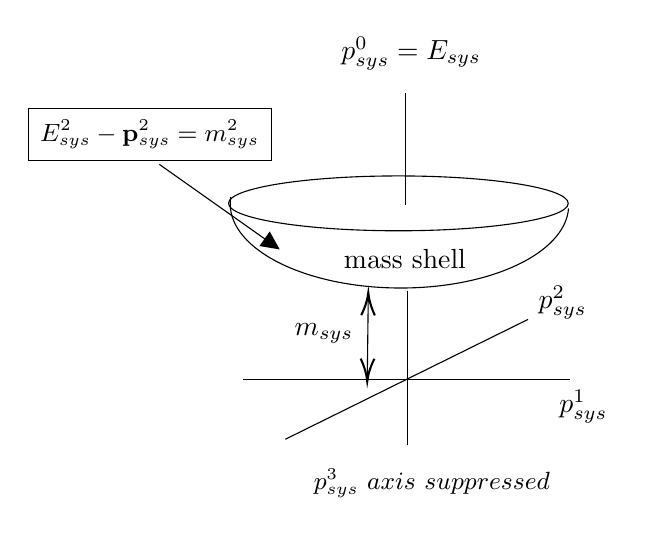
\begin{tikzpicture}[x=0.75pt,y=0.75pt,yscale=-1,xscale=1]
%uncomment if require: \path (0,300); %set diagram left start at 0, and has height of 300

%Shape: Ellipse [id:dp5571456664169634] 
\draw   (405,104.58) .. controls (405,97.28) and (441.64,91.37) .. (486.83,91.37) .. controls (532.03,91.37) and (568.67,97.28) .. (568.67,104.58) .. controls (568.67,111.88) and (532.03,117.8) .. (486.83,117.8) .. controls (441.64,117.8) and (405,111.88) .. (405,104.58) -- cycle ;
%Shape: Arc [id:dp5755134037737296] 
\draw  [draw opacity=0] (568.82,107.06) .. controls (567.12,128.58) and (531.16,145.6) .. (487.13,145.37) .. controls (442.1,145.14) and (405.69,126.94) .. (405.81,104.73) .. controls (405.81,103.68) and (405.9,102.64) .. (406.06,101.61) -- (487.34,105.16) -- cycle ; \draw   (568.82,107.06) .. controls (567.12,128.58) and (531.16,145.6) .. (487.13,145.37) .. controls (442.1,145.14) and (405.69,126.94) .. (405.81,104.73) .. controls (405.81,103.68) and (405.9,102.64) .. (406.06,101.61) ;
%Straight Lines [id:da112253833250195] 
\draw    (490.34,51.59) -- (490.34,105.16) ;
%Straight Lines [id:da11852275241679622] 
\draw    (491.34,146.59) -- (491.34,220.8) ;
%Straight Lines [id:da8670761805887259] 
\draw    (412,189.37) -- (569.67,189.37) ;
%Straight Lines [id:da3801545380094623] 
\draw    (432.38,218.24) -- (549.29,160.5) ;
%Straight Lines [id:da8071395461508041] 
\draw    (471.86,188.37) -- (472.32,149.59) ;
\draw [shift={(472.34,147.59)}, rotate = 450.68] [color={rgb, 255:red, 0; green, 0; blue, 0 }  ][line width=0.75]    (10.93,-3.29) .. controls (6.95,-1.4) and (3.31,-0.3) .. (0,0) .. controls (3.31,0.3) and (6.95,1.4) .. (10.93,3.29)   ;
\draw [shift={(471.83,190.37)}, rotate = 270.68] [color={rgb, 255:red, 0; green, 0; blue, 0 }  ][line width=0.75]    (10.93,-3.29) .. controls (6.95,-1.4) and (3.31,-0.3) .. (0,0) .. controls (3.31,0.3) and (6.95,1.4) .. (10.93,3.29)   ;
%Straight Lines [id:da37867462769054516] 
\draw    (371.67,85.8) -- (427.22,125.07) ;
\draw [shift={(429.67,126.8)}, rotate = 215.26] [fill={rgb, 255:red, 0; green, 0; blue, 0 }  ][line width=0.08]  [draw opacity=0] (8.93,-4.29) -- (0,0) -- (8.93,4.29) -- cycle    ;

% Text Node
\draw (451,167.37) node    {$m_{sys}$};
% Text Node
\draw (490,131.37) node   [align=left] {mass shell};
% Text Node
\draw (576,202.37) node    {$p^{1}_{sys}$};
% Text Node
\draw (566,152.37) node    {$p^{2}_{sys}$};
% Text Node
\draw (493,32.37) node    {$p^{0}_{sys} =E_{sys}$};
% Text Node
\draw    (308.5,58.87) -- (425.5,58.87) -- (425.5,83.87) -- (308.5,83.87) -- cycle  ;
\draw (367,71.37) node  [font=\small]  {$E^{2}_{sys} -\mathbf{p}^{2}_{sys} =m^{2}_{sys}$};
% Text Node
\draw (503,239.37) node  [font=\small]  {$p^{3}_{sys} \ axis\ suppressed$};


\end{tikzpicture}

\end{center}
The schematic above shows the following relation:(i.e. a shell upon which real particle energies and 3-momenta values must lie.)
\begin{equation}
E_{s y s}^{2}-\mathbf{p}_{s y s}^{2}=m_{s y s}^{2}
\end{equation}
For a system of particles, we determine an invariant mass $m_{sys}$. The surface in the figure is called the \textbf{mass shell}. Real particles must be "on the mass shell". Virtual particles can be, and generally are "off shell". $m_{sys}=0$ for photons, so the photon mass shell touches the origin.

From the delta function in (\ref{S-1-fi}), we know that the outgoing 4-momentum for the photon of Fig(\ref{fig:single-vertex}) equals the incoming total 4-momentum of the electron and positron:
$$
p_{i}^{\mu}=\left(\begin{array}{l}
{E_{1}+E_{2}} \\
{\mathbf{p}_{1}+\mathbf{p}_{2}}
\end{array}\right)=p_{f}^{\mu}=\left(\begin{array}{c}
{\omega_{k_{1}}} \\
{\mathbf{k}_{1}}
\end{array}\right)
$$
For initial state
$$
p_{i}^{\mu} p_{i \mu}=\left(E_{1}+E_{2}\right)^{2}-\left(\mathbf{p}_{1}+\mathbf{p}_{2}\right) \cdot\left(\mathbf{p}_{1}+\mathbf{p}_{2}\right)=m_{s y s}^{2} \neq 0
$$
For final state
$$
p_{f}^{\mu} p_{f \mu}=\underbrace{\left(E_{1}+E_{2}\right)^{2}}_{\omega_{\mathrm{k}_{1}}}-\underbrace{\left(\mathrm{p}_{1}+\mathrm{p}_{2}\right)}_{\mathrm{k}_{1}} \cdot \underbrace{\left(\mathrm{p}_{1}+\mathrm{p}_{2}\right)}_{\mathrm{k}_{1}}=m_{\mathrm{sys}}^{2} \neq 0
$$
\textbf{which must equal zero for a photon. That it doesn't equal zero means we can't produce a real photon.}
\begin{qt}
    $$
S_{f i}=\left\langle\gamma\left|S_{1}^{(1)} +\underbrace{S_{2}^{(1)}+\ldots+S_{8}^{(1)}}_{\text {all yield zero }}\right| e_{\mathbf{p}_{1}, n}^{-}, e_{\mathbf{p}_{2}, r_{2}}^{+}\right\rangle=\underbrace{\langle\gamma|}_{\text {on-shell }} \underbrace{\left.S_{1}^{(1)} | e_{p_{1}, n}^{-}, e^{+}_{\mathrm{p}_{2}, r_{2}}\right\rangle}_{\text {off-shell photon }}=0
$$
because the only ket left is an off-shell photon with $k^{\mu}=p_{1}^{\mu}+p_{2}^{\mu},$ and that is a different state from, and thus orthogonal to, any real final state photon, which cannot have this value for $k^{\mu} .$ Thus, the transition amplitude for Fig. (\ref{fig:single-vertex}) is zero. Similar logic for all single vertex interactions means we can simply ignore $S^{(1)}$ from here on.
\end{qt}
\section{Physical Meaning of S(2)}
\textbf{$S^{(2)}$ will represent two vertex interactions.} The first term of $S^{(2)}$ is $S_A^{(2)}$:
$$
S_{A}^{(2)}=-\frac{1}{2 !} e^{2} \iint d^{4} x_{1} d^{4} x_{2} N\left\{(\bar{\psi} \cancel{A} \psi)_{x_{1}}(\bar{\psi} \cancel{A} \psi)_{x_{2}}\right\}
$$
\textbf{\redp{This represents two independent processes like $S^{(1)}$.}} The two processes
do not interact with one another and each behaves as if the other did not exist. There is no virtual particle (Feynman propagator) linking them. Think of two separate single vertex Feynman diagrams. Neither of these can occur, so $S_A^{(2)}$ does not represent a real physical process and is ignored in QFT.

\subsection{The photon propagator term}
Consider the second term of $S^{(2)}$ acting on an initial state
\begin{equation}
S_{B}^{(2)}|i\rangle=-\frac{1}{2 !} e^{2} \iint d^{4} x_{1} d^{4} x_{2} N\left\{(\bar{\psi} \linktwoterms{\cancel{A}}{\psi)_{x_{1}}(\bar{\psi}}{\cancel{A}} \psi)_{x_{2}}\right\}|i\rangle
\label{four-external-lepton-interactions}
\end{equation}
The only initial states (\ref{four-external-lepton-interactions}) could destroy would be electron/positron states; and the only final states it could create would be electron/positron states. \textbf{We call these types of interactions four external lepton interactions.}
\begin{figure}[H]
    \centering
\tikzset{every picture/.style={line width=0.75pt}} %set default line width to 0.75pt        
\begin{tikzpicture}[x=0.75pt,y=0.75pt,yscale=-1,xscale=1]
%uncomment if require: \path (0,300); %set diagram left start at 0, and has height of 300

%Straight Lines [id:da29515338597014595] 
\draw    (39,63) -- (121.87,98.2) ;
%Straight Lines [id:da8356384809428652] 
\draw    (121.87,98.2) -- (42.87,149.2) ;
%Shape: Wave [id:dp48547110897765466] 
\draw   (121,97.7) .. controls (123.45,100.52) and (125.79,103.2) .. (128.5,103.2) .. controls (131.21,103.2) and (133.55,100.52) .. (136,97.7) .. controls (138.45,94.88) and (140.79,92.2) .. (143.5,92.2) .. controls (146.21,92.2) and (148.55,94.88) .. (151,97.7) .. controls (153.45,100.52) and (155.79,103.2) .. (158.5,103.2) .. controls (161.21,103.2) and (163.55,100.52) .. (166,97.7) .. controls (168.45,94.88) and (170.79,92.2) .. (173.5,92.2) .. controls (176.21,92.2) and (178.55,94.88) .. (181,97.7) .. controls (183.45,100.52) and (185.79,103.2) .. (188.5,103.2) .. controls (191.21,103.2) and (193.55,100.52) .. (196,97.7) .. controls (198.45,94.88) and (200.79,92.2) .. (203.5,92.2) .. controls (206.21,92.2) and (208.55,94.88) .. (211,97.7) .. controls (213.45,100.52) and (215.79,103.2) .. (218.5,103.2) .. controls (221.21,103.2) and (223.55,100.52) .. (226,97.7) .. controls (227.29,96.21) and (228.56,94.75) .. (229.87,93.72) ;
%Straight Lines [id:da12560516877601058] 
\draw    (308.87,43.2) -- (229.87,94.2) ;
%Straight Lines [id:da6163580842382406] 
\draw    (229.87,94.2) -- (312.73,129.4) ;
%Shape: Triangle [id:dp685466344952348] 
\draw  [fill={rgb, 255:red, 0; green, 0; blue, 0 }  ,fill opacity=1 ] (72.99,77.4) -- (89.03,81.1) -- (86.72,86.49) -- cycle ;
%Shape: Triangle [id:dp005741777290943051] 
\draw  [fill={rgb, 255:red, 0; green, 0; blue, 0 }  ,fill opacity=1 ] (263.86,108.6) -- (279.9,112.3) -- (277.58,117.69) -- cycle ;
%Shape: Triangle [id:dp11625025303653935] 
\draw  [fill={rgb, 255:red, 0; green, 0; blue, 0 }  ,fill opacity=1 ] (89.3,119.51) -- (76.95,130.4) -- (73.92,125.38) -- cycle ;
%Shape: Triangle [id:dp30589288901509604] 
\draw  [fill={rgb, 255:red, 0; green, 0; blue, 0 }  ,fill opacity=1 ] (276.3,64.51) -- (263.95,75.4) -- (260.92,70.38) -- cycle ;
%Straight Lines [id:da5797267371251957] 
\draw    (392.67,27.2) -- (516.67,60.2) ;
%Straight Lines [id:da5534129518575254] 
\draw    (516.67,60.2) -- (580.67,86.2) ;
%Straight Lines [id:da13099665104403413] 
\draw    (393.67,123.2) -- (466.67,101.2) ;
%Straight Lines [id:da23142398769308015] 
\draw    (466.67,101.2) -- (573.67,103.2) ;
%Shape: Triangle [id:dp9580604600019759] 
\draw  [fill={rgb, 255:red, 0; green, 0; blue, 0 }  ,fill opacity=1 ] (438,110.15) -- (423.07,117.08) -- (421.59,111.41) -- cycle ;
%Shape: Triangle [id:dp6776790710702215] 
\draw  [fill={rgb, 255:red, 0; green, 0; blue, 0 }  ,fill opacity=1 ] (542.27,103.15) -- (526.08,106.18) -- (526.05,100.32) -- cycle ;
%Shape: Wave [id:dp647042217139919] 
\draw   (519.94,62.74) .. controls (517.3,62.05) and (514.78,61.39) .. (513.37,62.52) .. controls (511.95,63.64) and (512.03,66.24) .. (512.11,68.97) .. controls (512.2,71.7) and (512.28,74.3) .. (510.86,75.42) .. controls (509.45,76.55) and (506.93,75.89) .. (504.29,75.2) .. controls (501.65,74.51) and (499.14,73.85) .. (497.72,74.98) .. controls (496.3,76.1) and (496.38,78.7) .. (496.47,81.43) .. controls (496.55,84.16) and (496.63,86.76) .. (495.22,87.88) .. controls (493.8,89.01) and (491.28,88.35) .. (488.64,87.66) .. controls (486.01,86.96) and (483.49,86.31) .. (482.07,87.43) .. controls (480.66,88.56) and (480.74,91.16) .. (480.82,93.89) .. controls (480.91,96.61) and (480.98,99.21) .. (479.57,100.34) .. controls (478.15,101.47) and (475.64,100.81) .. (473,100.12) .. controls (470.36,99.42) and (467.84,98.77) .. (466.43,99.89) .. controls (466.19,100.08) and (466,100.31) .. (465.84,100.58) ;
%Shape: Triangle [id:dp3657896804062972] 
\draw  [fill={rgb, 255:red, 0; green, 0; blue, 0 }  ,fill opacity=1 ] (446.78,41.87) -- (463.22,42.67) -- (461.89,48.39) -- cycle ;
%Shape: Triangle [id:dp26512090066334226] 
\draw  [fill={rgb, 255:red, 0; green, 0; blue, 0 }  ,fill opacity=1 ] (541.06,70.42) -- (557.28,73.22) -- (555.27,78.73) -- cycle ;
%Straight Lines [id:da8555170327907058] 
\draw    (258.77,230.2) -- (433.77,230.2) ;
\draw [shift={(436.77,230.2)}, rotate = 180] [fill={rgb, 255:red, 0; green, 0; blue, 0 }  ][line width=0.08]  [draw opacity=0] (8.93,-4.29) -- (0,0) -- (8.93,4.29) -- cycle    ;

% Text Node
\draw (59,53) node    {$p_{2}$};
% Text Node
\draw (72,148) node    {$p_{1}$};
% Text Node
\draw (291,36) node    {$p^{'}_{1}$};
% Text Node
\draw (294,141) node    {$p^{'}_{2}$};
% Text Node
\draw (121,117) node    {$x_{2}$};
% Text Node
\draw (233,117) node    {$x_{1}$};
% Text Node
\draw (177,74) node    {$k$};
% Text Node
\draw (529,41) node    {$x_{1}$};
% Text Node
\draw (472,119) node    {$x_{2}$};
% Text Node
\draw (573,53) node    {$p^{'}_{2}$};
% Text Node
\draw (568,120) node    {$p^{'}_{1}$};
% Text Node
\draw (480,69) node    {$k$};
% Text Node
\draw (406,104) node    {$p_{1}$};
% Text Node
\draw (403,48) node    {$p_{2}$};
% Text Node
\draw (178,182) node    {$S^{( 2)}_{B1}$};
% Text Node
\draw (485,182) node    {$S^{( 2)}_{B2}$};
% Text Node
\draw (351.33,220) node   [align=left] {time};


\end{tikzpicture}

    \caption{Bhabha scattering can occur in two ways}
    \label{fig:Bhabha-scattering}
\end{figure}
In Fig.(\ref{fig:Bhabha-scattering}), both scenarios have the same incoming and outgoing particle states, which are all that we can measure. The internal virtual particle interaction is not measurable so there is no way
we can tell which of the two interactions gave us the Bhabha scattering.Bhabha scattering actually entails both types of interaction, \bluep{i) an annihilation of $e^{-}$ with an $e^{+}$ followed by a creation of the same two types of particles,  and ii) one of the incoming particles emitting a virtual photon which is then absorbed by the other particle. i.e., the same incoming momenta and spins for both and the same outgoing momenta and spins for both.}

\subsubsection{First type of Bhabha Scattering}
Consider the first type of Bhabha scattering with the S operator acting on the incoming state,
\begin{equation}
S_{B}^{(2)}\left|e_{\mathrm{p}_{1}, \mathrm{r_1}}^{-}, e_{\mathrm{p}_{2}, \mathrm{r}_{2}}^{+}\right\rangle=-\frac{1}{2 !} e^{2} \iint d^{4} x_{1} d^{4} x_{2} N\left\{(\bar{\psi} \linktwoterms{\cancel{A}}{ \psi)_{x_{1}}(\bar{\psi}}{\cancel{A}}  \psi)_{x_{2}}\right\}\left|e_{\mathrm{p}_1, \mathrm{r}_1}^{-}, e^{+}_{\mathrm{p}_{2}, r_{2}}\right\rangle
\end{equation}
At $x_{2},$ the $\psi^{+}$ part of $\psi_{x_{2}}$ would destroy the ket electron; the $\bar{\psi}^+$ part of $\bar{\psi}_{x_{2}}$ would destroy the ket positron; and we would be left with the vacuum $|0\rangle$. The propagator would then create a virtual photon at $x_{2}$ and propagate it to $x_{1}$ where it would be destroyed. Then, the $\psi^{-}$ part of $\psi_{x_{1}}$ would create a positron at $x_{1} ;$ and the $\bar{\psi}$ part of $\bar{\psi}_{x_{1}}$ would create an electron there.
$$
S_{B 1}^{(2)}=\frac{-e^{2}}{2}\left\langle e^-_{p_{1}^{\prime}, r^{\prime}_1}, e^{+}_{ p_{2^{\prime}} r_{2}^{\prime}}\right|\iint d^{4} x_{1} d^{4} x_{2}\left((\bar{\psi}^{-} \linktwoterms{\cancel{A}}{ \psi^{-})_{x_{1}}(\bar{\psi}^{+}}{\cancel{A}} \psi^{+})_{x_{2}}+\right.
$$
$$
\left.N\left\{(\bar{\psi}^{+} \linktwoterms{\cancel{A}}{ \psi^{+})_{x_{1}}(\bar{\psi}^-}{\cancel{A}} \psi^{-})_{x_{2}}\right\}\right) \left| e_{\mathfrak{p}_{1}, r_{1}}^{-}, e^{+}_{\mathfrak{p}_{2}, r_{2}}\right\rangle
$$
in which we can think of the second term above as annihilation at $x_{1}$ and creation at $x_{2}$ instead of the other way around. When we normal order the second term, $\psi^{+}\left(x_{1}\right)$ is switched once with $\bar{\psi}^-$ ( $x_{2}$ ) introducing a minus sign, then switch order with $\psi^{-}\left(x_{2}\right),$ introducing a second minus sign and resulting in no total sign change. The propagator is just a number, so it can be moved anywhere without effect (though care
has to be taken with keeping the correct spinor multiplication order).

Carrying out similar switching for $\bar{\psi}^{+}\left(x_{1}\right)$ with $\bar{\psi}^{-}\left(x_{2}\right)$ and then $\psi^{-}\left(x_{2}\right),$ we end up with
$$
S_{B 1}^{(2)}=\frac{-e^{2}}{2}\left\langle e_{p_{1}^{\prime}, r^{\prime}_1}^-, e^{+}_{p_{2}^{\prime}, r_{2}^{\prime}}\right| \iint d^{4} x_{1} d^{4} x_{2}\left((\bar{\psi}^{-} \linktwoterms{\cancel{A}}{ \psi^{-})_{x_{1}}(\bar{\psi}^{+} }{\cancel{A}} \psi^{+})_{x_{2}}\right.+\left.(\bar{\psi}^{-} \linktwoterms{\cancel{A}}{ \psi^{-})_{x_{2}}(\bar{\psi}^{+}}{\cancel{A}} \psi^{+})_{x_{1}}\right)|\left.e_{p_{1}, r_1}^{-}, e^{+}_{p_{2}, r_{2}}\right\rangle
$$
$$
=-e^{2}\left\langle e_{p_{1}^{\prime}, r_1^{\prime}}^{-}, e^{+}_{p_{2}^{\prime}, r_{2}^{\prime}}\right| \iint d^{4} x_{1} d^{4} x_{2}(\bar{\psi}^{-} \linktwoterms{\cancel{A}}{ \psi^{-})_{x_{1}}(\bar{\psi}^{+}}{\cancel{A}} \psi^{+})_{x_{2}}\left|e_{\mathfrak{p}_{1}, r_1}^{-}, e_{p_{2}, r_{2}}^{+}\right\rangle
$$
\redp{where in second line we simply exchanged dummy variables in the second term of the first line to get the second line}. Substituting the field equation solutions for the operators at $x_2$ above, we have
$$
S_{B 1}^{(2)}=-e^{2}\left\langle e_{\mathrm{p}_{1}^{\prime}, r_1^{\prime}}^-, e_{\mathrm{p}_{2}^{\prime}, r_{2}}^{+}\right| \iint d^{4} x_{1} d^{4} x_{2}\left(\bar{\psi}^{-} \gamma^{\mu} \psi^{-}\right)_{x_{1}} i D_{F \mu \nu}\left(x_{1}-x_{2}\right) \times
$$
$$
\left(\sum_{r^{\prime}, p^{\prime}} \sqrt{\frac{m}{V E_{p'}}} d _{r'}\left(p^{\prime}\right) \bar{v}_{r^{\prime}}\left(p^{\prime}\right) e^{-i p^{\prime} x_{2}}\right) \gamma^{v}\left(\sum_{r^{\prime\prime} p^{\prime\prime}}, \sqrt{\frac{m}{V E_{p^{\prime\prime}}}} c_{r^{\prime\prime}}\left(\mathbf{p}^{\prime\prime}\right) u_{r^{\prime\prime}}\left(\mathbf{p}^{\prime \prime}\right) e^{-i p^{\prime\prime} \mathbf{x}_{2}}\right)\left|e_{\mathfrak{p}_{1}, r_{1}}^{-}, e^{+}_{\mathfrak{p}_{2}, r_{2}}\right\rangle
$$
The terms do match up turn the ket into the vacuum. So the equation above becomes
$$
S_{B 1}^{(2)}=-e^{2}\left\langle e^-_{\mathrm{p}_1^{\prime}, r_1^{\prime}}, e^{+}_{\mathrm{p}_{2}^{\prime}, r_{2}^{\prime}}\right| \iint d^{4} x_{1} d^{4} x_{2}\left(\bar{\psi}^{-} \gamma^{\mu} \psi^{-}\right)_{x_{1}} i D_{F \mu \nu}\left(x_{1}-x_{2}\right)\times
$$
$$
\frac{m}{V} \sqrt{\frac{1}{E_{\mathrm{p}_{1}} E_{\mathrm{p}_{2}}}} \bar{v}_{r_{2}}\left(\mathrm{p}_{2}\right) \gamma^{\nu} u_{r_{1}}\left(\mathrm{p}_{1}\right) e^{-i p_{2} x_{2}} e^{-i p_{1} x_{2}}|0\rangle
$$
Substituting the propagator relation we derived at the end of Chap 4 and rearranging,
$$
S_{B 1}^{(2)}=-e^{2}\left(e_{\mathrm{p}^{\prime} \mathrm{i}, \mathrm{r}^{\prime}}, e_{\mathrm{p}_{2}^{\prime}, \mathrm{r}_{2}^{\prime}}^{+} | \int\left(\bar{\psi}^{-} \gamma^{\mu} \psi^{-}\right)_{x_{1}} \times\right.\left(\int\left(\frac{-i g_{\mu \nu}}{(2 \pi)^{4}} \int \frac{e^{-i k\left(x_{1}-x_{2}\right)}}{k^{2}+i \varepsilon} d^{4} k\right) \frac{m}{V}\right.
$$
$$
\left.\sqrt{\frac{1}{E_{\mathrm{p}_{1}} E_{\mathrm{p}_{2}}}} \bar{v}_{r_{2}}\left(\mathrm{p}_{2}\right) \gamma^{v} u_{r_{1}}\left(\mathbf{p}_{1}\right) e^{-i p_{2} x_{2}} e^{-i p_{1} x_{2}} d^{4} x_{2}\right) d^{4} x_{1}|0\rangle
$$
$$
=e^{2}\left\langle e^-_{\mathrm{p}_{1}^{\prime}, r_{1}^{\prime}}, e_{\mathrm{p}_{2}^{\prime}, r_{2}^{\prime}}^{+}\right| \int\left(\bar{\psi}^- \gamma^{\mu} \psi^{-}\right)_{x_{1}} i g_{\mu \nu} \bar{v}_{r_{2}}\left(\mathbf{p}_{2}\right) \gamma^{\nu} u_{r_{1}}\left(\mathbf{p}_{1}\right) \times
$$
$$
\frac{m}{V} \sqrt{\frac{1}{E_{p_{1}} E_{p_{2}}}}\left(\int \frac{1}{k^{2}+i \varepsilon} e^{-i k x_{1}} \frac{1}{(2 \pi)^{4}}\underbrace{\left(\int e^{i k x_{2}} e^{-i p_{2} x_{2}} e^{-i p_{1} x_{2}} d^{4} x_{2}\right)}_{(2 \pi)^{4} \delta^{(4)}\left(k-p_{2}-p_{1}\right)} d^{4} k\right) d^{4} x_{1}|0\rangle
$$
\redp{The delta relation that results above tells us that $k=p_1+p_2$, the virtual photon 4-momentum equals th sum of the incoming particles 4-momenta. Again, we see conservation of energy and 3-momentum at a vertex.} \textbf{And again, we see that the photon particle is off-shell, i.e.,$k_{\mu}k^{\mu}=m^2_{sys}\neq0$.}

The delta relation picks the single value $k=p_1+p_2$ out of the integration over $k$. So now,
$$
S_{B 1}^{(2)}=e^{2}\left\langle e_{\mathrm{p}_{1}^{\prime}, r_{1}^{\prime}}^{-}, e_{\mathrm{p}_{2}^{\prime}, \mathrm{r}_{2}^{\prime}}^{+}\right| \frac{m}{V}\sqrt{\frac{1}{E_{\mathrm{p}_{1}} E_{\mathrm{p}_{2}}}}\left(\int\left(\bar{\psi}^- \gamma^{\mu} \psi^{-}\right)_{x_{1}} \frac{e^{-i\left(p_{2}+p_{1}\right) x_{1}}}{\left(p_{2}+p_{1}\right)^{2}+i \varepsilon} d^{4} x_{1}\right)\times$$
$$ i g_{\mu \nu}\bar{v}_{r_{2}}\left(\mathbf{p}_{2}\right) \gamma^{\nu} u_{r_{1}}\left(\mathbf{p}_{1}\right)|0\rangle
$$
Substituting the relations for the spinor creation field operators at $x_1$ yields
$$
S_{B 1}^{(2)}=e^{2}\left(\frac{m}{V}\right)^{2} \sqrt{\frac{1}{E_{\mathrm{p}_{1}} E_{\mathrm{p}_{2}}}} \sqrt{\frac{1}{E_{\mathrm{p}^{\prime}_{1}} E_{\mathrm{p}^{\prime}_{2}}}}\left\langle e_{\mathrm{p}_{1}^{\prime}, r_1^{\prime}}^{-}, e_{\mathrm{p}_{2}^{\prime}, \mathrm{r}_{2}^{\prime}}^{+}\right|\left(\int e^{-i\left(p_{2}+p_{1}\right) x_{1}} e^{i\left(p_{1}^{\prime}+p_{2}^{\prime}\right) x_{1}} d^{4} x_{1}\right) \times
$$
$$
\bar{u}_{r_{1}^{\prime}}\left(\mathbf{p}_{1}^{\prime}\right) \gamma^{\mu} v_{r_{2}^{\prime}}\left(\mathbf{p}_{2}^{\prime}\right) \frac{i g_{\mu v}}{\left(p_{2}+p_{1}\right)^{2}+i \varepsilon} \bar{v}_{r_{2}}\left(\mathbf{p}_{2}\right) \gamma^{v} u_{r_{1}}\left(\mathbf{p}_{1}\right)\left|e_{p_{1}^{\prime}, r_{1}^{\prime}}^-, e^{+}_{p_2^{\prime}, r_{2}^{\prime}}\right\rangle
$$
The integral over $x_{1}$ is another delta function telling us that $p_{2}^{\prime}+p^{\prime}_{1}=p_{2}+p_{1},$ the total outgoing $4$ -momentum equals the total incoming 4 -momentum, which, as we discovered earlier, equals the 4-momentum of the virtual photon propagator. Energy and 3 -momentum are conserved at every vertex. And the final, real particle state is on-shell.

The result of all this, where we note that the fraction factor in the equation above with the $i\varepsilon$ as part of the denominator is simply (up to a sign) the Feynman propagator in momentum space, is
\begin{qt}
    $$
\underbrace{S_{B 1}^{(2)}}_{\text { transition amplitude }}=\sqrt{\frac{m}{V E_{\mathrm{p}_1}}} \sqrt{\frac{m}{V E_{\mathrm{p}_2}}} \sqrt{\frac{m}{V E_{\mathrm{p}_1^{\prime}}}} \sqrt{\frac{m}{V E_{\mathrm{p}^{\prime}_{2}}}}(2 \pi)^{4} \delta^{(4)}\left(p_{1}+p_{2}-\left(p_{1}^{\prime}+p_{2}^{\prime}\right)\right)
$$
$$
\times \underbrace{\left(-e^{2}\right) \bar{u}_{r_{1}^{\prime}}\left(\mathbf{p}_{1}^{\prime}\right) \gamma^{\mu} v_{r_{2}^{\prime}}\left(\mathbf{p}_{2}^{\prime}\right) i D_{F \mu v}\left(k=p_{1}+p_{2}\right) \bar{v}_{r_{2}}\left(p_{2}\right) \gamma^{v} u_{r_{1}}\left(p_{1}\right)}_{\text {Feynman amplitude } \mathcal{M}_{B 1}^{(2)}}
$$
Note the definition of the Feynman amplitude for this interaction $\mathcal{M}_{B 1}^{(2)}$. Using that, we have
\begin{equation}
S_{B 1}^{(2)}=\left(\prod_{\mathbf{p}}^{\text {all ext fermions }} \sqrt{\frac{m}{V E_{\mathbf{p}}}}\right)(2 \pi)^{4} \delta^{(4)}\left(p_{1}+p_{2}-\left(p_{1}^{\prime}+p_{2}^{\prime}\right)\right) \mathcal{M}_{B 1}^{(2)}
\end{equation}
\end{qt}
\subsubsection{The second type of Bhabha scattering}
Note in Fig.(\ref{fig:Bhabha-scattering}), that on the RHS, either $x_2$ or $x_1$ could occur first, and our math takes care of both cases automatically. We start with the same fundamental relation we had for the first type of Bhabha scattering,
\begin{equation}
S_{B}^{(2)}\left|e_{\mathrm{p}_{1}, r_{1}}^{-}, e_{\mathrm{p}_{2}, r_{2}}^{+}\right\rangle=-\frac{e^{2}}{2!} \iint d^{4} x_{1} d^{4} x_{2} N\left\{(\bar{\psi} \linktwoterms{\cancel{A}}{ \psi)_{x_{1}}(\bar{\psi}}{\cancel{A} } \psi)_{x_{2}}\right\} \left| e_{\mathfrak{p}_{1},r_1}^-, e_{\mathrm{p}_{2}, \mathrm{r}_{2}}^{+}\right\rangle
\end{equation}
\textbf{\bluep{but this time, we pick the creation and destruction operators corresponding to the second type of
Bhabha scattering. That is, we have}}
$$
S^{(2)}_{B2}=\frac{-e^{2}}{2}\left\langle e^-_{p_{1}^{\prime}, r_{1}^{\prime}}, e^+_{p_{2}^{\prime}, r_{2}^{\prime}}\right| \times
$$
$$
\iint d^{4} x_{1} d^{4} x_{2} N\left\{(\bar{\psi}^{+} \linktwoterms{A_{\mu}}{ \gamma^{\mu} \psi^{-})_{x_{1}}(\bar{\psi}^{-}}{A_{v}} \gamma^{v} \psi^{+})_{x_{2}}+(\bar{\psi} \linktwoterms{A_{\mu}}{ \gamma^{\mu} \psi^{+})_{x_{1}}(\bar{\psi}^{+}}{ A_{v}} \gamma^{v} \psi^{-})_{x_{2}}\right\}\left|e_{\mathbf{p}_{1}, r_{1}}^{-}, e^{+}_{ \mathbf{p}_{2}, r_{2}}\right\rangle
$$
which, if \textbf{we switch dummy integration variables again, the first and second terms above are equivalent.} That eliminates the $1 / 2$ factor and leaves (where we now show spinor indices).
\begin{equation}
S_{B 2}^{(2)}=-e^{2}\langle e_{\mathrm{p}_{1}^{\prime}, r_{1}^{\prime}}^{-}, e^{+}_{\mathrm{p}_{2}^{\prime}, r_{2}^{\prime}}| \iint d^{4} x_{1} d^{4} x_{2} N \{(\bar{\psi}_{\alpha}^{+} \linktwoterms{A_{\mu}}{ \gamma_{\alpha \beta}^{\mu} \psi_{\beta}^{-})_{x_{1}}(\bar{\psi}_{\delta}^-}{ A_{\nu}} \gamma_{\delta \eta}^{\nu} \psi_{\eta}^{+})_{x_{2}}\} | e_{\mathrm{p}_{1}, r_{1}}^{-}, e_{\mathrm{p}_{2}, r_{2}}^{+}\rangle
\label{second-type-Bhabha}
\end{equation}
This can be visualized as the incoming electron destroyed at $x_{2}$ with the outgoing electron created a $x_{2}$ and a photon propagator starting at $x_{2}$. The incoming positron is destroyed at $x_{1}$ with the outgoing positron positron created at $x_{1}$ and the photon propagator ending at $x_{1}$. The reverse situation, where $x_{1}$ and $x_2$ are interchanged has been included by the factor of two enveloped.

Normal ordering (\ref{second-type-Bhabha}), where we now see the value of writing out spinor indices, give us
\begin{equation}
S_{B 2}^{(2)}=e^{2}\langle e_{p_{1}^{\prime}, r_1^{\prime}}^-, e^{+} _{p_2^{\prime}, r_{2}^{\prime}}| \iint d^{4} x_{1} d^{4} x_{2} (\bar{\psi}^{-}_{\delta})_{x_{2}}(\linktwoterms{A_{\mu}}{ \gamma_{\alpha \beta}^{\mu} \psi_{\beta}^{-})_{x_{1}}(\bar{\psi}_{\alpha}^{+})_{x_{1}}(}{A_{v}} \gamma_{\delta \eta}^{v} \psi_{\eta}^{+})_{x_{2}})|e_{p_{1}, r_1}^{-}, e^{+}_{p_{2}, r_{2}}\rangle
\label{second-type-Bhabha-scattering-2}
\end{equation}
Note carefully that we have to put (\ref{second-type-Bhabha-scattering-2}) not simply in any normal order, but \textbf{in the same normal order as (\ref{second-type-Bhabha}). That is, both transition sub amplitudes must have, in order from the right side moving leftward, operators performing $e^-$ destruction, $e^+$ destruction, $e^-$ creation, and $e^+$ creation.} We carry out similar steps to get
$$
S_{B 2}^{(2)}=e^{2} \frac{m^{2}}{V^{2}} \sqrt{\frac{1}{E_{\mathrm{p} 1} E_{\mathrm{p}_{2}} E_{\mathrm{p}_1^{\prime}} E_{\mathrm{p}_{2}^{\prime}}}} \bar{v}_{r_{2}}\left(\mathrm{p}_{2}\right) \gamma^{\mu} v_{r_{2}^{\prime}}\left(\mathbf{p}_{2}^{\prime}\right) \bar{u}_{\mathrm{r}^{\prime}}\left(\mathbf{p}_{\mathrm{I}}^{\prime}\right) \gamma^{v} u_{\mathrm{r}_{1}}\left(\mathbf{p}_{1}\right) \times
$$
$$
\left(\frac{-i g_{\mu \nu}}{\left(p_{1}-p_{1}^{\prime}\right)^{2}+i \varepsilon}\right) \underbrace{\left(\int e^{-i\left(p_{1}-p_{1}^{\prime}\right) x_{1}} e^{i p_{2}^{\prime} x_{1}} e^{-i p_{2} x_{1}} d^{4} x_{1}\right)}_{(2 \pi)^{4} \delta^{(4)}\left(p_{1}+p_{2}-\left(p_{1}^{\prime}+p_{2}^{\prime}\right)\right)}
$$
And thus, finally,
\begin{qt}
    \begin{equation}
S_{B 2}^{(2)}=\left(\prod_{\mathbf{p}}^{\text {allext fermions }} \sqrt{\frac{m}{V E_{\mathrm{p}}}}\right)(2 \pi)^{4} \delta^{(4)}\left(p_{1}+p_{2}-\left(p_{1}^{\prime}+p_{2}^{\prime}\right)\right) \mathcal{M}_{B 2}^{(2)}
\end{equation}
where
$$
\mathcal{M}_{B 2}^{(2)}=e^{2} \bar{v}_{r_{2}}\left(\mathbf{p}_{2}\right) \gamma^{\mu} v_{r^{\prime}_{2}}\left(\mathbf{p}_{2}^{\prime}\right) i D_{\mu v}\left(p_{2}^{\prime}-p_{2}\right) \bar{u}_{r_1^{\prime}}\left(\mathbf{p}_{1}^{\prime}\right) \gamma^{v} u_{r_1}\left(\mathbf{p}_{1}\right)
$$
\end{qt}
The total transition amplitude for 2nd order (n=2) Bhabha scatering is
\begin{equation}
S_{B h a b b a}=S_{B 1}^{(2)}+S_{B 2}^{(2)}=\left(\prod_{\mathrm{p}}^{\text {all fermions }} \frac{m}{\sqrt{\frac{m}{V E_{\mathrm{p}}}}}\right)(2 \pi)^{4} \delta^{(4)}\left(p_{1}+p_{2}-\left(p_{1}^{\prime}+p_{2}^{\prime}\right)\right)\left(\mathcal{M}_{B 1}^{(2)}+\mathcal{M}_{B 2}^{(2)}\right)
\end{equation}

\subsection{Compton Scattering}
Consider the third and fourth terms in $S^{(2)}$, acting on an initial state
\begin{equation}
S_{C}^{(2)}|i\rangle=-\frac{1}{2 !} e^{2} \iint d^{4} x_{1} d^{4} x_{2}(N\{(\bar{\psi} \linktwoterms{\cancel{A}}{ \psi)_{x_{1}}(\bar{\psi}}{\cancel{A}} \psi)_{x_{2}}\}+N\{(\bar{\psi}\linktwoterms{\cancel{A}}{ \psi)_{x_{1}}(\bar{\psi}}{\cancel{A}} \psi)_{x_{2}}\}) | i\rangle
\label{compton-scattering}
\end{equation}
The first term in (\ref{compton-scattering}) actually equals the second term as we can see from the following Box, and thus we can re-express (\ref{compton-scattering}) as
\begin{equation}
S_{C}^{(2)}|i\rangle=-\frac{1}{2 !} e^{2} \iint d^{4} x_{1} d^{4} x_{2}N\{(\bar{\psi}\linktwoterms{\cancel{A}}{ \psi)_{x_{1}}(\bar{\psi}}{\cancel{A}} \psi)_{x_{2}}\} | i\rangle
\label{compton-scattering-2}
\end{equation}
The contraction here is a fermion propagator and the incoming particles that could be destroyed by (\ref{compton-scattering-2}) could comprise an electron and a photon. Effectively, the electron and photon could scatter off one another as in Fig. (\ref{fig:compton-scattering}). This is called\textbf{ Compton scattering}. Note from Fig. (\ref{fig:compton-scattering}) than occur in two different ways, i.e., have the same real particles in and out.
\begin{figure}[H]
    \centering

\tikzset{every picture/.style={line width=0.75pt}} %set default line width to 0.75pt        

\begin{tikzpicture}[x=0.75pt,y=0.75pt,yscale=-1,xscale=1]
%uncomment if require: \path (0,300); %set diagram left start at 0, and has height of 300

%Straight Lines [id:da9652866719093866] 
\draw    (42,138.93) -- (235.87,138.93) ;
%Shape: Wave [id:dp4726907497917253] 
\draw   (57.65,100.38) .. controls (57.52,103.46) and (57.41,106.39) .. (58.9,107.41) .. controls (60.39,108.44) and (63.08,107.27) .. (65.9,106.03) .. controls (68.72,104.8) and (71.42,103.63) .. (72.91,104.65) .. controls (74.4,105.68) and (74.28,108.61) .. (74.16,111.68) .. controls (74.03,114.76) and (73.91,117.69) .. (75.4,118.71) .. controls (76.9,119.73) and (79.59,118.57) .. (82.41,117.33) .. controls (85.23,116.1) and (87.92,114.93) .. (89.41,115.95) .. controls (90.9,116.98) and (90.79,119.91) .. (90.66,122.98) .. controls (90.53,126.06) and (90.41,128.99) .. (91.9,130.01) .. controls (93.4,131.03) and (96.09,129.86) .. (98.91,128.63) .. controls (101.73,127.4) and (104.42,126.23) .. (105.91,127.25) .. controls (107.41,128.27) and (107.29,131.21) .. (107.16,134.28) .. controls (107.09,135.86) and (107.03,137.39) .. (107.19,138.65) ;
%Shape: Wave [id:dp581219954893428] 
\draw   (174.65,139.38) .. controls (174.52,142.46) and (174.41,145.39) .. (175.9,146.41) .. controls (177.39,147.44) and (180.08,146.27) .. (182.9,145.03) .. controls (185.72,143.8) and (188.42,142.63) .. (189.91,143.65) .. controls (191.4,144.68) and (191.28,147.61) .. (191.16,150.68) .. controls (191.03,153.76) and (190.91,156.69) .. (192.4,157.71) .. controls (193.9,158.73) and (196.59,157.57) .. (199.41,156.33) .. controls (202.23,155.1) and (204.92,153.93) .. (206.41,154.95) .. controls (207.9,155.98) and (207.79,158.91) .. (207.66,161.98) .. controls (207.53,165.06) and (207.41,167.99) .. (208.9,169.01) .. controls (210.4,170.03) and (213.09,168.86) .. (215.91,167.63) .. controls (218.73,166.4) and (221.42,165.23) .. (222.91,166.25) .. controls (224.41,167.27) and (224.29,170.21) .. (224.16,173.28) .. controls (224.09,174.86) and (224.03,176.39) .. (224.19,177.65) ;
%Shape: Triangle [id:dp4781339171474417] 
\draw  [fill={rgb, 255:red, 0; green, 0; blue, 0 }  ,fill opacity=1 ] (74.65,139.08) -- (58.25,142.65) -- (58.19,135.79) -- cycle ;
%Shape: Triangle [id:dp052309184229321404] 
\draw  [fill={rgb, 255:red, 0; green, 0; blue, 0 }  ,fill opacity=1 ] (147.15,138.86) -- (130.75,142.44) -- (130.69,135.57) -- cycle ;
%Shape: Triangle [id:dp3157602553829544] 
\draw  [fill={rgb, 255:red, 0; green, 0; blue, 0 }  ,fill opacity=1 ] (218.15,138.86) -- (201.75,142.44) -- (201.69,135.57) -- cycle ;
%Straight Lines [id:da7163286367875737] 
\draw    (276,138.93) -- (469.87,138.93) ;
%Shape: Wave [id:dp35829325317941596] 
\draw   (368.65,100.38) .. controls (368.52,103.46) and (368.41,106.39) .. (369.9,107.41) .. controls (371.39,108.44) and (374.08,107.27) .. (376.9,106.03) .. controls (379.72,104.8) and (382.42,103.63) .. (383.91,104.65) .. controls (385.4,105.68) and (385.28,108.61) .. (385.16,111.68) .. controls (385.03,114.76) and (384.91,117.69) .. (386.4,118.71) .. controls (387.9,119.73) and (390.59,118.57) .. (393.41,117.33) .. controls (396.23,116.1) and (398.92,114.93) .. (400.41,115.95) .. controls (401.9,116.98) and (401.79,119.91) .. (401.66,122.98) .. controls (401.53,126.06) and (401.41,128.99) .. (402.9,130.01) .. controls (404.4,131.03) and (407.09,129.86) .. (409.91,128.63) .. controls (412.73,127.4) and (415.42,126.23) .. (416.91,127.25) .. controls (418.41,128.27) and (418.29,131.21) .. (418.16,134.28) .. controls (418.09,135.86) and (418.03,137.39) .. (418.19,138.65) ;
%Shape: Wave [id:dp7598034423297523] 
\draw   (321.65,139.38) .. controls (321.52,142.46) and (321.41,145.39) .. (322.9,146.41) .. controls (324.39,147.44) and (327.08,146.27) .. (329.9,145.03) .. controls (332.72,143.8) and (335.42,142.63) .. (336.91,143.65) .. controls (338.4,144.68) and (338.28,147.61) .. (338.16,150.68) .. controls (338.03,153.76) and (337.91,156.69) .. (339.4,157.71) .. controls (340.9,158.73) and (343.59,157.57) .. (346.41,156.33) .. controls (349.23,155.1) and (351.92,153.93) .. (353.41,154.95) .. controls (354.9,155.98) and (354.79,158.91) .. (354.66,161.98) .. controls (354.53,165.06) and (354.41,167.99) .. (355.9,169.01) .. controls (357.4,170.03) and (360.09,168.86) .. (362.91,167.63) .. controls (365.73,166.4) and (368.42,165.23) .. (369.91,166.25) .. controls (371.41,167.27) and (371.29,170.21) .. (371.16,173.28) .. controls (371.09,174.86) and (371.03,176.39) .. (371.19,177.65) ;
%Shape: Triangle [id:dp8027556070300854] 
\draw  [fill={rgb, 255:red, 0; green, 0; blue, 0 }  ,fill opacity=1 ] (308.65,139.08) -- (292.25,142.65) -- (292.19,135.79) -- cycle ;
%Shape: Triangle [id:dp27556888831393467] 
\draw  [fill={rgb, 255:red, 0; green, 0; blue, 0 }  ,fill opacity=1 ] (381.15,138.86) -- (364.75,142.44) -- (364.69,135.57) -- cycle ;
%Shape: Triangle [id:dp8251492979907598] 
\draw  [fill={rgb, 255:red, 0; green, 0; blue, 0 }  ,fill opacity=1 ] (452.15,138.86) -- (435.75,142.44) -- (435.69,135.57) -- cycle ;
%Straight Lines [id:da46165972339858774] 
\draw    (192,239.93) -- (326.17,239.93) ;
\draw [shift={(329.17,239.93)}, rotate = 180] [fill={rgb, 255:red, 0; green, 0; blue, 0 }  ][line width=0.08]  [draw opacity=0] (8.93,-4.29) -- (0,0) -- (8.93,4.29) -- cycle    ;

% Text Node
\draw (48,153.93) node    {$p$};
% Text Node
\draw (232,122.93) node    {$p^{'}$};
% Text Node
\draw (236,185.93) node    {$k^{'}$};
% Text Node
\draw (66,86.93) node    {$k$};
% Text Node
\draw (130,211.93) node    {$S^{( 2)}_{C1}$};
% Text Node
\draw (282,153.93) node    {$p$};
% Text Node
\draw (466,122.93) node    {$p^{'}$};
% Text Node
\draw (383,185.93) node    {$k^{'}$};
% Text Node
\draw (377,86.93) node    {$k$};
% Text Node
\draw (364,211.93) node    {$S^{( 2)}_{C2}$};
% Text Node
\draw (263,228.93) node   [align=left] {time};


\end{tikzpicture}

    \caption{Compton Scattering Can Occur in Two Ways}
    \label{fig:compton-scattering}
\end{figure}
The LH vertex on each side of Fig.(\ref{fig:compton-scattering}) with $x_2$, and the RH with $x_1$, as it would be easier to track the analysis. The interaction could occur in either of the ways we label above as $S_{C 1}^{(2)}$ or $S_{C 2}^{(2)} .$ That is, either i) an electron could absorb a photon (equivalent to an electron and a photon being destroyed and a virtual electron being created at $x_{2}$ ) and later emit a photon(equivalent to the virtual electron being destroyed and both a real electron and a real photon being created at $x_1$); or ii) an electron could emit a photon (equivalent to an electron being destroyed and a real photon along with a virtual electron being created at $x_2$), and later absorbed a photo (equivalent to the virtual electron and a real photon being destroyed while a real electron is create at $x_1$).

\redp{Note that only the $S_{C}^{(2)}$ terms of all the $n=2$ terms will result in destruction of an initial electron and photon ket. }The $S$ matrix transition amplitude for second order Compton scattering is thus (with incoming particles unprimed, outgoing primed)
\begin{equation}
S_{\text {Compton }}=\langle f|S| i\rangle=\left\langle e^-_{\mathbf{p}^{\prime}, s^{\prime}}, \gamma_{\mathbf{k}^{\prime} r^{\prime}}\left|\left(-e^{2}\right) \iint d^{4} x_{1} d^{4} x_{2} N \int\left((\vec{\psi} \linktwoterms{\cancel{A}}{ \psi)_{x_{1}}(\bar{\psi}}{\cancel{A}} \psi)_{x_{2}}\right)\right| e_{\mathbf{p}, s}^{-}, \gamma_{\mathbf{k}, r}\right\rangle
\end{equation}
\begin{equation}
=-e^{2}\left\langle e^-_{\mathbf{p}^{\prime} s^{\prime}}, \gamma_{\mathbf{k}^{\prime}, r^{\prime}}\right| \iint d^{4} x_{1} d^{4} x_{2} N\left\{\left(\bar{\psi}^{+}+\bar{\psi}^{-}\right)_{x_{1}}\left(\cancel{A}^{+}+\cancel{A}^{-}\right)_{x_{1}} \times\right.
\end{equation}
$$
\left.\left(i S_{F}\left(x_{1}-x_{2}\right)\right)\left(\cancel{A}^{+}+\cancel{A}^{-}\right)_{x_{2}}\left(\psi^{+}+\psi^{-}\right)_{x_{2}}\right\}\left|e_{\mathbf{p}, s}^{-}, \gamma_{\mathbf{k}, r}\right\rangle
$$
After the operators raise and lower the ket, only two terms in the equation above remain:
\begin{equation}
\begin{split}
S_{\text {Compton }}&=-e^{2}\left\langle e^-_{\mathbf{p}^{\prime}, s^{\prime}}, \gamma_{\mathbf{k}^{\prime}, r^{\prime}}\right| \iint d^{4} x_{1} d^{4} x_{2} \underbrace{N\left\{\bar{\psi}_{x_{1}}^{-} \cancel{A}_{x_{1}}^{-}\left(i S_{F}\left(x_{1}-x_{2}\right)\right) \cancel{A}_{x_{2}}^{+} \psi_{x_{2}}^{+}\right.}_
{S_{C 1}^{(2)} \text { term } }\\
&+\underbrace{\bar{\psi}_{x_{1}}^{-} \cancel{A}_{x_{1}}^{+}\left(i S_{F}\left(x_{1}-x_{2}\right)\right) \cancel{A}_{x_{2}}^{-} \psi_{x_{2}}^{+}}_{\text {will result in } S_{C_{2}}^{(2)} \text { term }}\}\left|e_{\mathbf{p}, s}^{-}, \gamma_{\mathbf{k}, r}\right\rangle
\end{split}
\end{equation}
\begin{qt}
    The full second order Compton transition amplitude, including both cases of Fig.(\ref{fig:compton-scattering}), is
    \begin{equation}
    \begin{split}
        S_{\text {Compton }}&=\left(\prod_{\mathbf{p}^{''}}^{\text {all fermions }} \sqrt{\frac{m}{V E_{\mathrm{p}^{''}}}}\right)\left(\prod_{\mathbf{p}^{''}}^{\text {all bosons }} \sqrt{\frac{1}{2 V \omega_{\mathbf{k}^{\prime\prime}}}}\right)(2 \pi)^{4}\times\\
        &\delta^{(4)}\left(p^{\prime}+k^{\prime}-p-k\right)\left(\mathcal{M}_{C 1}^{(2)}+\mathcal{M}_{C 2}^{(2)}\right)
    \end{split}
\end{equation}
where
$$
\mathcal{M}_{C 1}^{(2)}=-e^{2} \bar{u}_{s^{\prime}, \alpha}\left(\mathbf{p}^{\prime}\right) \varepsilon_{\mu, r^{\prime}}\left(\mathbf{k}^{\prime}\right) \gamma_{\alpha \beta}^{\mu} i S_{F \beta \delta}(q=p+k) \varepsilon_{\nu, r}(\mathbf{k}) \gamma_{\delta \eta}^{\nu} u_{s, \eta}(\mathbf{p})
$$
$$
\mathcal{M}_{C 2}^{(2)}=-e^{2} \bar{u}_{s^{\prime}, \alpha}\left(\mathbf{p}^{\prime}\right) \varepsilon_{\mu, r}(\mathbf{k}) \gamma_{\alpha \beta}^{\mu} i S_{F \beta \delta}\left(q=p-k^{\prime}\right) \varepsilon_{\nu, r^{\prime}}\left(\mathbf{k}^{\prime}\right) \gamma_{\delta \eta}^{\nu} u_{s, \eta}(\mathbf{p})
$$
\end{qt}
\begin{mybox}
Consider normal ordering the commutator of two boson fields which do not commute,such as
$$
N \underbrace{\left[\phi^{+}\left(x_{1}\right), \phi^{\dagger-}\left(x_{2}\right)\right]}_{\neq 0}=N\left\{\phi^{+}\left(x_{1}\right) \phi^{\dagger-}\left(x_{2}\right)-\phi^{\dagger-}\left(x_{2}\right) \phi^{+}\left(x_{1}\right)\right\}=\phi^{\dagger-}\left(x_{2}\right) \phi^{+}\left(x_{1}\right)-\phi^{\dagger-}\left(x_{2}\right) \phi^{+}\left(x_{1}\right)=0
$$
Similarly, the normal ordering of an anti-commutator of two fermion fields, which do not anti-commute, equals zero as well. \textbf{Thus, we can simply exchange order of adjacent bosons inside any normal ordered product, even if they don't commute and even if they are part of a contraction.} For example
$$
N\left\{\phi\left(x_{1}\right) \phi^{\dagger}\left(x_{2}\right) \psi\left(x_{3}\right) \bar{\psi}\left(x_{4}\right) \dots\right\}$$
$$=N\left\{\left(\phi^{\dagger}\left(x_{2}\right) \phi\left(x_{1}\right)+\underbrace{\left[\phi\left(x_{1}\right), \phi^{\dagger}\left(x_{2}\right)\right]}_{\text {drops out}}\right) \psi\left(x_{3}\right) \bar{\psi}\left(x_{4}\right) \dots\right\}
$$
$$
=N\left\{\phi^{\dagger}\left(x_{2}\right) \phi\left(x_{1}\right) \psi\left(x_{3}\right) \bar{\psi}\left(x_{4}\right) \dots\right\}
$$
Similarly, we can exchange the order of adjacent fermion fields, along with a sign change, inside any normal ordered product. Fermion and adjacent bosons always commute.With the above results, we can re-order factors in the first term of $S c^{(2)}$
$$
N\{(\linktwoterms{\bar{\psi}_{\alpha}}{ A_{\mu} \gamma_{\alpha \beta}^{\mu} \psi_{\beta})_{x_{1}}(\bar{\psi}_{\delta} A_{\nu} \gamma_{\delta \eta}^{\nu}}{ \psi_{\eta}})_{x_{2}}\}=N\{(\bar{\psi}_{\delta})_{x_{2}}(\linktwoterms{\bar{\psi}_{\alpha}}{ A_{\mu} \gamma_{\alpha \beta}^{\mu} \psi_{\beta})_{x_{1}}(A_{\nu} \gamma_{\delta \eta}^{\nu}}{ \psi_{\eta})_{x_{2}}}\}=
$$
$$
N\left\{\left(\bar{\psi}_{\delta} A_{v} \gamma_{\delta \eta}^{v}\right)_{x_{2}}(\linktwoterms{\bar{\psi}_{\alpha}}{ A_{\mu} \gamma_{\alpha \beta}^{\mu} \psi_{\beta})_{x_{1}}(}{\psi_{\eta}})_{x_{2}}\right\}=N\left\{\left(\bar{\psi}_{\delta} A_{v} \gamma_{\delta \eta}^{v}\right)_{x_{2}}(\linktwoterms{\bar{\psi}_{\alpha}}{)_{x_{1}}(}{\psi_{\eta}})_{x_{2}}\left(-A_{\mu} \gamma_{\alpha \beta}^{\mu} \psi_{\beta}\right)_{x_{1}}\right\}
$$
$$
=N\left\{(\bar{\psi}_{\delta} A_{v} \gamma_{\delta \eta}^{\nu} \linktwoterms{\psi_{\eta}}{)_{x_{2}}(}{\bar{\psi}_{\alpha}} A_{\mu} \gamma_{\alpha \beta}^{\mu} \psi_{\beta})_{x_{1}}\right\}
$$
the $x_1$ and $x_2$ are dummy variables so we can make the exchange $x_{1} \leftrightarrow x_{2}$
\end{mybox}
\subsection{Returning to the Photon Propagator Term \texorpdfstring{$S_B^{(2)}$}{TEXT}}
Similar to Compton and Bhabha scattering, there are two ways for Moller scattering (see the figure below) to occur in which the outgoing electrons have the same individual momenta (and spins). And since we can only measure the incoming and outgoing particles, we have no way of knowing which of the two may have occurred. We thus must add the two amplitudes to get the total amplitude.
\begin{figure}[H]
    \centering

\tikzset{every picture/.style={line width=0.75pt}} %set default line width to 0.75pt        

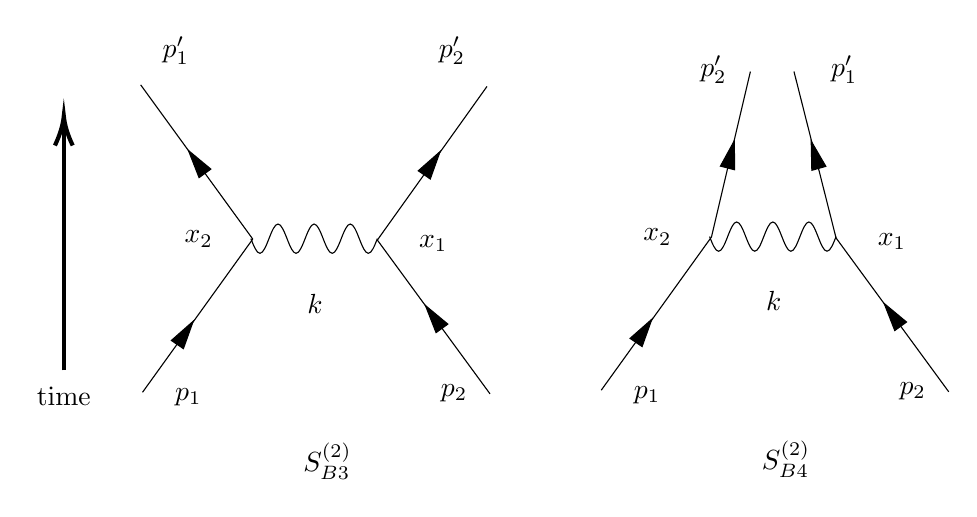
\begin{tikzpicture}[x=0.75pt,y=0.75pt,yscale=-1,xscale=1]
%uncomment if require: \path (0,300); %set diagram left start at 0, and has height of 300

%Straight Lines [id:da9046977999285625] 
\draw    (67.03,42.7) -- (121.04,117.01) ;
%Straight Lines [id:da06100511569815992] 
\draw    (121.04,117.01) -- (67.93,190.83) ;
%Shape: Wave [id:dp2673899563513945] 
\draw   (120.14,116.82) .. controls (121.56,120.43) and (122.91,123.87) .. (124.49,123.87) .. controls (126.06,123.87) and (127.42,120.43) .. (128.84,116.82) .. controls (130.26,113.21) and (131.62,109.77) .. (133.19,109.77) .. controls (134.77,109.77) and (136.13,113.21) .. (137.55,116.82) .. controls (138.97,120.43) and (140.32,123.87) .. (141.9,123.87) .. controls (143.47,123.87) and (144.83,120.43) .. (146.25,116.82) .. controls (147.67,113.21) and (149.03,109.77) .. (150.6,109.77) .. controls (152.18,109.77) and (153.54,113.21) .. (154.96,116.82) .. controls (156.38,120.43) and (157.73,123.87) .. (159.31,123.87) .. controls (160.88,123.87) and (162.24,120.43) .. (163.66,116.82) .. controls (165.08,113.21) and (166.44,109.77) .. (168.01,109.77) .. controls (169.59,109.77) and (170.95,113.21) .. (172.37,116.82) .. controls (173.79,120.43) and (175.14,123.87) .. (176.72,123.87) .. controls (178.3,123.87) and (179.65,120.43) .. (181.07,116.82) ;
%Straight Lines [id:da6329057798671613] 
\draw    (235.35,191.59) -- (181.07,117.48) ;
%Straight Lines [id:da680948881222658] 
\draw    (181.07,117.48) -- (233.9,43.46) ;
%Straight Lines [id:da4348608997197827] 
\draw [line width=1.5]    (30,180.27) -- (30,60.7) ;
\draw [shift={(30,57.7)}, rotate = 450] [color={rgb, 255:red, 0; green, 0; blue, 0 }  ][line width=1.5]    (14.21,-4.28) .. controls (9.04,-1.82) and (4.3,-0.39) .. (0,0) .. controls (4.3,0.39) and (9.04,1.82) .. (14.21,4.28)   ;
%Shape: Triangle [id:dp7748544979530381] 
\draw  [fill={rgb, 255:red, 0; green, 0; blue, 0 }  ,fill opacity=1 ] (92.34,156.6) -- (87.62,169.79) -- (81.83,165.86) -- cycle ;
%Shape: Triangle [id:dp6024942312731019] 
\draw  [fill={rgb, 255:red, 0; green, 0; blue, 0 }  ,fill opacity=1 ] (211.29,74.86) -- (206.57,88.05) -- (200.78,84.12) -- cycle ;
%Shape: Triangle [id:dp7430747380130274] 
\draw  [fill={rgb, 255:red, 0; green, 0; blue, 0 }  ,fill opacity=1 ] (204.24,149.03) -- (215.02,157.98) -- (209.35,162.08) -- cycle ;
%Shape: Triangle [id:dp5887628847311597] 
\draw  [fill={rgb, 255:red, 0; green, 0; blue, 0 }  ,fill opacity=1 ] (90.06,74.35) -- (100.84,83.3) -- (95.17,87.4) -- cycle ;
%Straight Lines [id:da9758876191029576] 
\draw    (360.8,36.3) -- (342.04,116.01) ;
%Straight Lines [id:da14762447663048084] 
\draw    (342.04,116.01) -- (288.93,189.83) ;
%Shape: Wave [id:dp35880322334435466] 
\draw   (341.14,115.82) .. controls (342.56,119.43) and (343.91,122.87) .. (345.49,122.87) .. controls (347.06,122.87) and (348.42,119.43) .. (349.84,115.82) .. controls (351.26,112.21) and (352.62,108.77) .. (354.19,108.77) .. controls (355.77,108.77) and (357.13,112.21) .. (358.55,115.82) .. controls (359.97,119.43) and (361.32,122.87) .. (362.9,122.87) .. controls (364.47,122.87) and (365.83,119.43) .. (367.25,115.82) .. controls (368.67,112.21) and (370.03,108.77) .. (371.6,108.77) .. controls (373.18,108.77) and (374.54,112.21) .. (375.96,115.82) .. controls (377.38,119.43) and (378.73,122.87) .. (380.31,122.87) .. controls (381.88,122.87) and (383.24,119.43) .. (384.66,115.82) .. controls (386.08,112.21) and (387.44,108.77) .. (389.01,108.77) .. controls (390.59,108.77) and (391.95,112.21) .. (393.37,115.82) .. controls (394.79,119.43) and (396.14,122.87) .. (397.72,122.87) .. controls (399.3,122.87) and (400.65,119.43) .. (402.07,115.82) ;
%Straight Lines [id:da07517307957898689] 
\draw    (456.35,190.59) -- (402.07,116.48) ;
%Straight Lines [id:da31330503553681854] 
\draw    (402.07,116.48) -- (381.8,36.3) ;
%Shape: Triangle [id:dp7411050182023194] 
\draw  [fill={rgb, 255:red, 0; green, 0; blue, 0 }  ,fill opacity=1 ] (313.34,155.6) -- (308.62,168.79) -- (302.83,164.86) -- cycle ;
%Shape: Triangle [id:dp81021383639529] 
\draw  [fill={rgb, 255:red, 0; green, 0; blue, 0 }  ,fill opacity=1 ] (390.1,69.86) -- (397.14,81.97) -- (390.4,83.87) -- cycle ;
%Shape: Triangle [id:dp5708438164475254] 
\draw  [fill={rgb, 255:red, 0; green, 0; blue, 0 }  ,fill opacity=1 ] (425.24,148.03) -- (436.02,156.98) -- (430.35,161.08) -- cycle ;
%Shape: Triangle [id:dp5376275039059243] 
\draw  [fill={rgb, 255:red, 0; green, 0; blue, 0 }  ,fill opacity=1 ] (353.09,69.58) -- (353.14,83.59) -- (346.36,81.87) -- cycle ;

% Text Node
\draw (90,193.27) node    {$p_{1}$};
% Text Node
\draw (218,191.27) node    {$p_{2}$};
% Text Node
\draw (84,26.27) node    {$p^{\prime }_{1}$};
% Text Node
\draw (217,26.27) node    {$p^{\prime }_{2}$};
% Text Node
\draw (95,117) node    {$x_{2}$};
% Text Node
\draw (208,119) node    {$x_{1}$};
% Text Node
\draw (151,148) node    {$k$};
% Text Node
\draw (157,224) node    {$S^{( 2)}_{B3}$};
% Text Node
\draw (311,192.27) node    {$p_{1}$};
% Text Node
\draw (439,190.27) node    {$p_{2}$};
% Text Node
\draw (343,35.27) node    {$p^{\prime }_{2}$};
% Text Node
\draw (406,35.27) node    {$p^{\prime }_{1}$};
% Text Node
\draw (316,116) node    {$x_{2}$};
% Text Node
\draw (429,118) node    {$x_{1}$};
% Text Node
\draw (372,147) node    {$k$};
% Text Node
\draw (378,223) node    {$S^{( 2)}_{B4}$};
% Text Node
\draw (30,192.87) node   [align=left] {time};


\end{tikzpicture}

    \caption{Moller Scattering}
    \label{fig:moller-scattering}
\end{figure}
In finding the result, take care to note that either $x_{1}$ or $x_{2}$ can occur first and this is already accounted for in the Dyson time ordering converted, via Wick's theorem, to normal ordering.

A separate issue is that in our expression for the transition amplitude, \textbf{the $p_{2}$ electron could be destroyed at $x_{2}$ instead of $x_{1}$ (and vice versa for the $p_{1}$ electron).} If you work the math you will see these are two different terms, each of which contributes to the amplitude. However, they have the same form if we simply switch dummy integration variables $x_{2} \leftrightarrow x_{1}$ in one of them. Hence, we will get two equal terms for the LHS of Fig. \ref{fig:moller-scattering} and two equal terms for the RHS. This allow us to use only one of them for the LHS and one for the RHS, but multiply the transition amplitude expression by 2. The final results are
\begin{equation}
\left.S_{M o l l e r}=\left(\prod_{\mathbf{p}}^{\text {all fermions}}\right) \sqrt{\frac{m}{V E_{p}}}\right)(2 \pi)^{4} \delta^{(4)}\left(p_{1}^{\prime}+p_{2}^{\prime}-p_{1}-p_{2}\right)\left(\mathcal{M}_{B 3}^{(2)}+\mathcal{M}_{B 4}^{(2)}\right)
\end{equation}
\begin{equation}
\begin{aligned}
&\mathcal{M}_{B 3}^{(2)}=+e^{2} \bar{u}_{r_1^{\prime}}\left(\mathbf{p}_{1}^{\prime}\right) \gamma^{\mu} u_{r_1}\left(\mathbf{p}_{1}\right) i D_{F \mu \nu}\left(k=p_{1}-p_{1}^{\prime}\right) \bar{u}_{r_{2}^{\prime}}\left(\mathbf{p}_{2}^{\prime}\right) \gamma^{\nu} u_{r_{2}}\left(\mathbf{p}_{2}\right)\\
&\mathcal{M}_{B 4}^{(2)}=-e^{2} \bar{u}_{r_{2}^{\prime}}\left(\mathbf{p}_{2}^{\prime}\right) \gamma^{\mu} u_{r_{1}}\left(\mathbf{p}_{1}\right) i D_{F \mu \nu}\left(k=p_{1}-p_{2}^{\prime}\right) \bar{u}_{r_{1}^{\prime}}\left(\mathbf{p}_{1}^{\prime}\right) \gamma^{v} u_{r_{2}}\left(\mathbf{p}_{2}\right)
\end{aligned}
\end{equation}
In the process of finding $\mathcal{M}_{B 3}^{(2)},$ we have to normal order. In so doing, we put the destruction operators $\psi^{+}\left(p_{1}\right)$ and $\psi^{+}\left(\mathbf{p}_{2}\right)$ at the end. But they could be ordered there as $\psi^{+}\left(p_{1}\right) \psi^{+}\left(p_{2}\right),$ or as $\psi^{+}\left(p_{2}\right) \psi^{+}\left(p_{1}\right) .$ Either would be correct normal order, but the sign of the resulting amplitude would be different. \redp{\textbf{The key is that in finding $\mathcal{M}_{B 4}^{(2)},$ we have to normal order in the same order as we did for. $\mathcal{M}_{B 3}^{(2)}$}}.

\subsection{The Electron/Positron Closed Loop Term \texorpdfstring{$S_D^{(2)}$}{TEXT}}
For the closed loop terms, we have
\begin{equation}
S_{D}^{(2)}=-\frac{1}{2 !} e^{2} \iint d^{4} x_{1} d^{4} x_{2}(N \left\{\linktwotermsl{\bar{\psi}}{\linktwoterms{\cancel{A}}{ \psi)_{x_{1}}(\bar{\psi}}{\cancel{A}} }{\psi})_{x_{2}}\right\}+N\left\{(\bar{\psi} \linktwotermsl{\cancel{A}}{ \linktwoterms{\psi}{)_{x_{1}}(}{\bar{\psi}}}{ \cancel{A}} \psi)_{x_{2}}\right\})
\label{electron-close-loop}
\end{equation}
In the manner detailed in the Box above, we can reorder either of these by switching adjacent fields (and introducing a minus sign each time we switch fermions). Doing this to the first term makes it look like the second term. Thus, (\ref{electron-close-loop}) becomes
\begin{equation}
S_{D}^{(2)}=-e^{2} \iint d^{4} x_{1} d^{4} x_{2}N\left\{(\bar{\psi} \linktwotermsl{\cancel{A}}{ \linktwoterms{\psi}{)_{x_{1}}(}{\bar{\psi}}}{ \cancel{A}} \psi)_{x_{2}}\right\}
\label{electron-close-loop2}
\end{equation}
which is represented by the following Feynman diagram
\begin{figure}[H]
    \centering
\tikzset{every picture/.style={line width=0.75pt}} %set default line width to 0.75pt        
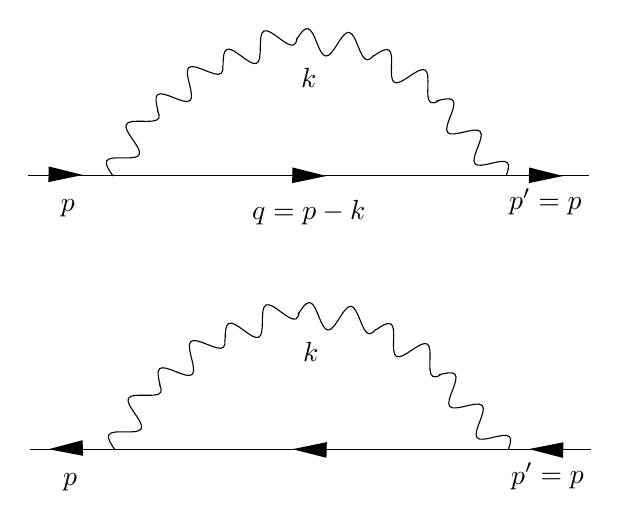
\begin{tikzpicture}[x=0.75pt,y=0.75pt,yscale=-1,xscale=1]
%uncomment if require: \path (0,300); %set diagram left start at 0, and has height of 300

%Straight Lines [id:da3309419816061372] 
\draw    (55.87,111.2) -- (325.87,111.2) ;
%Shape: Wave [id:dp1690099098873552] 
\draw   (96.77,111.45) .. controls (94.75,108.52) and (92.83,105.72) .. (93.68,104.12) .. controls (94.54,102.53) and (97.94,102.58) .. (101.5,102.64) .. controls (105.07,102.7) and (108.46,102.76) .. (109.32,101.16) .. controls (110.18,99.57) and (108.25,96.77) .. (106.23,93.83) .. controls (104.2,90.89) and (102.28,88.09) .. (103.14,86.5) .. controls (103.99,84.9) and (107.39,84.96) .. (110.96,85.02) .. controls (114.52,85.08) and (117.92,85.13) .. (118.77,83.54) .. controls (119.25,82.64) and (118.86,81.37) .. (118.06,79.9) ;
%Shape: Wave [id:dp6849760876199679] 
\draw   (118.44,80.2) .. controls (117.59,76.73) and (116.78,73.43) .. (118.15,72.24) .. controls (119.51,71.06) and (122.67,72.31) .. (125.98,73.63) .. controls (129.3,74.95) and (132.45,76.21) .. (133.82,75.02) .. controls (135.18,73.83) and (134.38,70.53) .. (133.53,67.07) .. controls (132.68,63.61) and (131.87,60.31) .. (133.24,59.12) .. controls (134.6,57.93) and (137.76,59.18) .. (141.07,60.51) .. controls (144.39,61.83) and (147.54,63.08) .. (148.91,61.89) .. controls (149.68,61.23) and (149.76,59.9) .. (149.53,58.24) ;
%Shape: Wave [id:dp4145403198216897] 
\draw   (149.75,58.16) .. controls (149.81,54.6) and (149.87,51.2) .. (151.49,50.4) .. controls (153.11,49.59) and (155.85,51.61) .. (158.72,53.73) .. controls (161.58,55.85) and (164.32,57.86) .. (165.94,57.06) .. controls (167.56,56.26) and (167.62,52.86) .. (167.68,49.3) .. controls (167.74,45.73) and (167.8,42.33) .. (169.42,41.53) .. controls (171.04,40.73) and (173.78,42.74) .. (176.64,44.86) .. controls (179.51,46.98) and (182.25,49) .. (183.87,48.2) .. controls (184.78,47.75) and (185.2,46.48) .. (185.4,44.82) ;
%Shape: Wave [id:dp37643260046922233] 
\draw   (184.87,46.06) .. controls (186.78,43.05) and (188.61,40.18) .. (190.41,40.34) .. controls (192.21,40.51) and (193.49,43.66) .. (194.83,46.96) .. controls (196.16,50.27) and (197.45,53.41) .. (199.25,53.58) .. controls (201.05,53.74) and (202.88,50.88) .. (204.79,47.87) .. controls (206.7,44.86) and (208.52,41.99) .. (210.33,42.15) .. controls (212.13,42.32) and (213.41,45.46) .. (214.75,48.77) .. controls (216.08,52.08) and (217.36,55.22) .. (219.17,55.39) .. controls (220.18,55.48) and (221.2,54.62) .. (222.23,53.31) ;
%Shape: Wave [id:dp9599988483851968] 
\draw   (222.15,53.63) .. controls (225.11,51.64) and (227.93,49.75) .. (229.51,50.62) .. controls (231.1,51.49) and (231.01,54.89) .. (230.9,58.45) .. controls (230.8,62.02) and (230.71,65.42) .. (232.29,66.29) .. controls (233.88,67.16) and (236.7,65.27) .. (239.66,63.28) .. controls (242.62,61.3) and (245.44,59.41) .. (247.03,60.28) .. controls (248.61,61.15) and (248.52,64.55) .. (248.41,68.11) .. controls (248.31,71.68) and (248.22,75.08) .. (249.8,75.95) .. controls (250.69,76.44) and (251.97,76.06) .. (253.45,75.28) ;
%Shape: Wave [id:dp887728068451431] 
\draw   (252.66,75.14) .. controls (256.07,74.33) and (259.31,73.57) .. (260.5,74.93) .. controls (261.69,76.29) and (260.5,79.41) .. (259.24,82.67) .. controls (257.98,85.93) and (256.78,89.05) .. (257.97,90.41) .. controls (259.16,91.77) and (262.41,91.01) .. (265.81,90.2) .. controls (269.22,89.4) and (272.46,88.64) .. (273.65,90) .. controls (274.84,91.36) and (273.65,94.48) .. (272.39,97.74) .. controls (271.13,101) and (269.93,104.12) .. (271.12,105.48) .. controls (272.31,106.84) and (275.56,106.08) .. (278.96,105.27) .. controls (282.37,104.47) and (285.61,103.71) .. (286.8,105.07) .. controls (287.75,106.16) and (287.18,108.37) .. (286.26,110.89) ;
%Shape: Triangle [id:dp7611450922119929] 
\draw  [fill={rgb, 255:red, 0; green, 0; blue, 0 }  ,fill opacity=1 ] (80.93,110.85) -- (65.86,113.98) -- (66.01,107.11) -- cycle ;
%Shape: Triangle [id:dp16707753725067276] 
\draw  [fill={rgb, 255:red, 0; green, 0; blue, 0 }  ,fill opacity=1 ] (198.37,111.35) -- (183.3,114.48) -- (183.44,107.61) -- cycle ;
%Shape: Triangle [id:dp18464177276205462] 
\draw  [fill={rgb, 255:red, 0; green, 0; blue, 0 }  ,fill opacity=1 ] (312.37,111.35) -- (297.3,114.48) -- (297.44,107.61) -- cycle ;
%Straight Lines [id:da2482645667024742] 
\draw    (56.87,243.2) -- (326.87,243.2) ;
%Shape: Wave [id:dp7204922677035164] 
\draw   (97.77,243.45) .. controls (95.75,240.52) and (93.83,237.72) .. (94.68,236.12) .. controls (95.54,234.53) and (98.94,234.58) .. (102.5,234.64) .. controls (106.07,234.7) and (109.46,234.76) .. (110.32,233.16) .. controls (111.18,231.57) and (109.25,228.77) .. (107.23,225.83) .. controls (105.2,222.89) and (103.28,220.09) .. (104.14,218.5) .. controls (104.99,216.9) and (108.39,216.96) .. (111.96,217.02) .. controls (115.52,217.08) and (118.92,217.13) .. (119.77,215.54) .. controls (120.25,214.64) and (119.86,213.37) .. (119.06,211.9) ;
%Shape: Wave [id:dp3337602221620415] 
\draw   (119.44,212.2) .. controls (118.59,208.73) and (117.78,205.43) .. (119.15,204.24) .. controls (120.51,203.06) and (123.67,204.31) .. (126.98,205.63) .. controls (130.3,206.95) and (133.45,208.21) .. (134.82,207.02) .. controls (136.18,205.83) and (135.38,202.53) .. (134.53,199.07) .. controls (133.68,195.61) and (132.87,192.31) .. (134.24,191.12) .. controls (135.6,189.93) and (138.76,191.18) .. (142.07,192.51) .. controls (145.39,193.83) and (148.54,195.08) .. (149.91,193.89) .. controls (150.68,193.23) and (150.76,191.9) .. (150.53,190.24) ;
%Shape: Wave [id:dp4347619235507304] 
\draw   (150.75,190.16) .. controls (150.81,186.6) and (150.87,183.2) .. (152.49,182.4) .. controls (154.11,181.59) and (156.85,183.61) .. (159.72,185.73) .. controls (162.58,187.85) and (165.32,189.86) .. (166.94,189.06) .. controls (168.56,188.26) and (168.62,184.86) .. (168.68,181.3) .. controls (168.74,177.73) and (168.8,174.33) .. (170.42,173.53) .. controls (172.04,172.73) and (174.78,174.74) .. (177.64,176.86) .. controls (180.51,178.98) and (183.25,181) .. (184.87,180.2) .. controls (185.78,179.75) and (186.2,178.48) .. (186.4,176.82) ;
%Shape: Wave [id:dp18507857213489687] 
\draw   (185.87,178.06) .. controls (187.78,175.05) and (189.61,172.18) .. (191.41,172.34) .. controls (193.21,172.51) and (194.49,175.66) .. (195.83,178.96) .. controls (197.16,182.27) and (198.45,185.41) .. (200.25,185.58) .. controls (202.05,185.74) and (203.88,182.88) .. (205.79,179.87) .. controls (207.7,176.86) and (209.52,173.99) .. (211.33,174.15) .. controls (213.13,174.32) and (214.41,177.46) .. (215.75,180.77) .. controls (217.08,184.08) and (218.36,187.22) .. (220.17,187.39) .. controls (221.18,187.48) and (222.2,186.62) .. (223.23,185.31) ;
%Shape: Wave [id:dp02539109071774759] 
\draw   (223.15,185.63) .. controls (226.11,183.64) and (228.93,181.75) .. (230.51,182.62) .. controls (232.1,183.49) and (232.01,186.89) .. (231.9,190.45) .. controls (231.8,194.02) and (231.71,197.42) .. (233.29,198.29) .. controls (234.88,199.16) and (237.7,197.27) .. (240.66,195.28) .. controls (243.62,193.3) and (246.44,191.41) .. (248.03,192.28) .. controls (249.61,193.15) and (249.52,196.55) .. (249.41,200.11) .. controls (249.31,203.68) and (249.22,207.08) .. (250.8,207.95) .. controls (251.69,208.44) and (252.97,208.06) .. (254.45,207.28) ;
%Shape: Wave [id:dp4254288717826974] 
\draw   (253.66,207.14) .. controls (257.07,206.33) and (260.31,205.57) .. (261.5,206.93) .. controls (262.69,208.29) and (261.5,211.41) .. (260.24,214.67) .. controls (258.98,217.93) and (257.78,221.05) .. (258.97,222.41) .. controls (260.16,223.77) and (263.41,223.01) .. (266.81,222.2) .. controls (270.22,221.4) and (273.46,220.64) .. (274.65,222) .. controls (275.84,223.36) and (274.65,226.48) .. (273.39,229.74) .. controls (272.13,233) and (270.93,236.12) .. (272.12,237.48) .. controls (273.31,238.84) and (276.56,238.08) .. (279.96,237.27) .. controls (283.37,236.47) and (286.61,235.71) .. (287.8,237.07) .. controls (288.75,238.16) and (288.18,240.37) .. (287.26,242.89) ;
%Shape: Triangle [id:dp2499057150249553] 
\draw  [fill={rgb, 255:red, 0; green, 0; blue, 0 }  ,fill opacity=1 ] (66.94,242.96) -- (81.81,239.01) -- (82.05,245.87) -- cycle ;
%Shape: Triangle [id:dp7780285755044771] 
\draw  [fill={rgb, 255:red, 0; green, 0; blue, 0 }  ,fill opacity=1 ] (184.37,243.03) -- (199.44,239.94) -- (199.29,246.8) -- cycle ;
%Shape: Triangle [id:dp6157200253057087] 
\draw  [fill={rgb, 255:red, 0; green, 0; blue, 0 }  ,fill opacity=1 ] (298.37,242.97) -- (313.47,240) -- (313.26,246.86) -- cycle ;

% Text Node
\draw (191,64) node    {$k$};
% Text Node
\draw (305,124) node    {$p^{\prime } =p$};
% Text Node
\draw (75,127) node    {$p$};
% Text Node
\draw (191,129) node    {$q=p-k$};
% Text Node
\draw (192,196) node    {$k$};
% Text Node
\draw (306,256) node  [rotate=-359.69]  {$p^{\prime } =p$};
% Text Node
\draw (76,259) node    {$p$};


\end{tikzpicture}
    \caption{Electron Closed Loop(top) and Positron Closed Loop(bottom)}
    \label{fig:electron-positron-closed-loop}
\end{figure}
\textbf{The dosed loop diagrams are also called self-energy diagrams.} In Fig.\ref{fig:electron-positron-closed-loop}, with closed loops, however, one of the virtual particles' 4-momentum can be anything. That is, for any value of $k$(the virtual photon 4-momentum),$q$ simply takes on the value $q=p-k$. The sum total of $k$ and $q$ must equal $p$, but this does not determine $k$ and $q$ separately. \redp{Thus, we need to integrate the expression for the transition amplitude of Fig.\ref{fig:electron-positron-closed-loop} over all values of $k$} i.e., over all values of $k^{0}$ from $-\infty$ to $+\infty$, and all yalues of $\mathbf{k}$ from $-\infty$ to $\infty$ along all three spatial directions.
$$
S_{\text {eloop}}=\left\langle e_{\mathbf{p}^{\prime}, s^{\prime}}\left|S_{D}^{(2)}\right|{e_{\mathbf{p}, s}^-}\right\rangle
$$
$$
=\left\langle e^-_{\mathbf{p}^{\prime} . s^{\prime}}\left|-e^{2} \iint d^{4} x_{1} d^{4} x_{2} i D_{F \mu \nu}\left(x_{1}-x_{2}\right)(\bar{\psi}^-)_{x_{1}} \gamma^{\mu} i S_{F}\left(x_{1}-x_{2}\right) \gamma^{\nu}\left(\psi^{+}\right)_{x_{2}}\right| e_{\mathbf{p} . s}^{-}\right\rangle
$$
$$
=-e^{2}\left\langle e_{p^{\prime}, s}^{-}\right| \iint d^{4} x_{1} d^{4} x_{2} i D_{F \mu \nu}\left(x_{1}-x_{2}\right)\left(\sum_{\mathbf{p}^{\prime}, s^{\prime\prime}} \sqrt{\frac{m}{V E_{p^{\prime \prime}}} \bar{u}_{s^{\prime\prime}}}\left(\mathbf{p}^{\prime \prime}\right) c_{s^{\prime\prime}}^{\dagger}\left(\mathbf{p}^{\prime\prime}\right) e^{i p^{\prime\prime} x_{1}}\right) \gamma^{\mu} \times
$$
$$
i S_{F}\left(x_{1}-x_{2}\right) \gamma^{\nu} \sqrt{\frac{m}{V E_{p}}} u_{s}(\mathbf{p}) e^{-i p x_{2}}|0\rangle
$$
Re-arranging factors, \textbf{\bluep{and integrate over spatial coordinates, we have}}
$$
S_{\text {e loop }}=-e^{2} \iint d^{4} q d^{4} k\left(\frac{1}{(2 \pi)^{4}}\right) \underbrace{\left(\frac{-i g_{\mu \nu}}{k^{2}+i \varepsilon}\right)}_{i D_{\mu \nu}(k)}\underbrace{\left(\int e^{-i kx_{1}} e^{-i q x_{1}} e^{i p_{1}^{\prime}x_1} d^{4} x_{1}\right)}_{(2 \pi)^{4} \delta^{(4)}\left(q-\left(p^{\prime}-k\right)\right)}\underbrace{\left(\int e^{i k x_{2}} e^{i q x_{2}} e^{-i p x_{2}} d^{4} x_{2}\right)}_{(2 \pi)^{4} \delta^{(4)}(q-(p-k))}\times
$$
$$
\frac{m}{V} \sqrt{\frac{1}{E_{p^{\prime}} E_{p}}} \bar{u}_{s^{\prime}}\left(\mathbf{p}^{\prime}\right) \gamma^{\mu} \frac{1}{(2 \pi)^{4}} \underbrace{i\left(\frac{(\not q+m)}{q^{2}-m^{2}+i \varepsilon}\right)}_{i S_{F}(q)} \gamma^{\nu} u_{s}(\mathbf{p})
$$
With the Dirac delta functions, integration over $q$ leaves $p^{\prime}-k=p-k$, meaning $p^{\prime}=p$, and thus,
$$
S_{e l o o p}=-e^{2} \delta^{(4)}\left(p-p^{\prime}=0\right) \frac{m}{V E_{p}} \int d^{4} k i D_{F \mu \nu}(k) \bar{u}_{s^{\prime}}(p) \gamma^{\mu} i S_{F}(p-k) \gamma^{\nu} u_{s}(p)
$$
We can show that only the $s=s^{\prime}$ spin state survives. Thus, the electron loop transition amplitude is
\begin{qt}
    \begin{equation}
S_{e l o o p}=\prod_{\mathbf{p}^{\prime}}^{\text {all fermions }} \sqrt{\frac{m}{V E_{p^{\prime}}}}(2 \pi)^{4} \delta^{(4)}\left(p-p^{\prime}\right) \mathcal{M}_{e l o o p}
\end{equation}
where
\begin{equation}
\mathcal{M}_{e l o o p}=\frac{-e^{2}}{(2 \pi)^{4}} \int d^{4} k i D_{F \mu \nu}(k) \bar{u}_{s}(\mathbf{p}) \gamma^{\mu} i S_{F}(p-k) \gamma^{\nu} u_{s}(\mathbf{p})
\end{equation}
\end{qt}

\subsection{The Photon Closed Loop Term \texorpdfstring{$S_E^{(2)}$}{TEXT}}
Like the electron, the photon has a closed loop interaction:
\begin{equation}
S_{E}^{(2)}=-\frac{1}{2 !} e^{2} \iint d^{4} x_{1} d^{4} x_{2} N \left\{(\linktwotermsl{\bar{\psi}}{ \cancel{A} \linktwoterms{\psi}{)_{x_{1}}(}{\bar{\psi}} \cancel{A}}{ \psi})_{x_{2}}\right\}
\label{photon-closed-loop}
\end{equation}
As presented by the Feynman diagram of Fig.\ref{fig:photon-closed-loop}, the photon closed loop (or self-energy) diagram is also known as a \redp{vacuum polarization loop} diagram because, in it, the chargeless photon sitting in the vacuum is polarized, i.e., it split into a particle with plus(pole) charge and a particle with negative (pole) charge.
\begin{figure}[H]
    \centering

\tikzset{every picture/.style={line width=0.75pt}} %set default line width to 0.75pt        

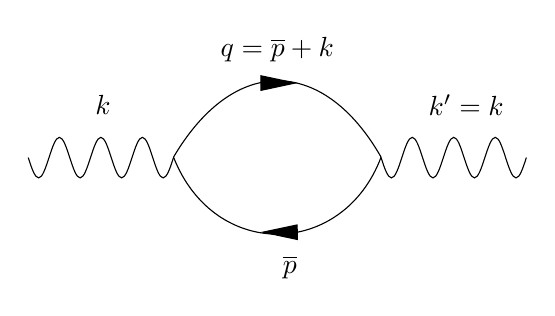
\begin{tikzpicture}[x=0.75pt,y=0.75pt,yscale=-1,xscale=1]
%uncomment if require: \path (0,300); %set diagram left start at 0, and has height of 300

%Shape: Wave [id:dp03799766308452357] 
\draw   (69,148.23) .. controls (70.63,153.24) and (72.19,158) .. (74,158) .. controls (75.81,158) and (77.37,153.24) .. (79,148.23) .. controls (80.63,143.23) and (82.19,138.47) .. (84,138.47) .. controls (85.81,138.47) and (87.37,143.23) .. (89,148.23) .. controls (90.63,153.24) and (92.19,158) .. (94,158) .. controls (95.81,158) and (97.37,153.24) .. (99,148.23) .. controls (100.63,143.23) and (102.19,138.47) .. (104,138.47) .. controls (105.81,138.47) and (107.37,143.23) .. (109,148.23) .. controls (110.63,153.24) and (112.19,158) .. (114,158) .. controls (115.81,158) and (117.37,153.24) .. (119,148.23) .. controls (120.63,143.23) and (122.19,138.47) .. (124,138.47) .. controls (125.81,138.47) and (127.37,143.23) .. (129,148.23) .. controls (130.63,153.24) and (132.19,158) .. (134,158) .. controls (135.81,158) and (137.37,153.24) .. (139,148.23) ;
%Curve Lines [id:da03627181894428755] 
\draw    (139,148) .. controls (168.87,97.47) and (211.87,100.47) .. (239,148) ;
%Curve Lines [id:da8952061471565331] 
\draw    (139,148) .. controls (158.87,198.47) and (220.87,196.47) .. (239,148) ;
%Shape: Wave [id:dp9595032443711723] 
\draw   (239,148.23) .. controls (240.63,153.24) and (242.19,158) .. (244,158) .. controls (245.81,158) and (247.37,153.24) .. (249,148.23) .. controls (250.63,143.23) and (252.19,138.47) .. (254,138.47) .. controls (255.81,138.47) and (257.37,143.23) .. (259,148.23) .. controls (260.63,153.24) and (262.19,158) .. (264,158) .. controls (265.81,158) and (267.37,153.24) .. (269,148.23) .. controls (270.63,143.23) and (272.19,138.47) .. (274,138.47) .. controls (275.81,138.47) and (277.37,143.23) .. (279,148.23) .. controls (280.63,153.24) and (282.19,158) .. (284,158) .. controls (285.81,158) and (287.37,153.24) .. (289,148.23) .. controls (290.63,143.23) and (292.19,138.47) .. (294,138.47) .. controls (295.81,138.47) and (297.37,143.23) .. (299,148.23) .. controls (300.63,153.24) and (302.19,158) .. (304,158) .. controls (305.81,158) and (307.37,153.24) .. (309,148.23) ;
%Shape: Triangle [id:dp9825029435409027] 
\draw  [fill={rgb, 255:red, 0; green, 0; blue, 0 }  ,fill opacity=1 ] (197.6,112.3) -- (181.17,115.81) -- (181.1,108.81) -- cycle ;
%Shape: Triangle [id:dp365323645361745] 
\draw  [fill={rgb, 255:red, 0; green, 0; blue, 0 }  ,fill opacity=1 ] (182.13,184.15) -- (198.57,180.67) -- (198.63,187.67) -- cycle ;

% Text Node
\draw (105,123) node    {$k$};
% Text Node
\draw (280,123) node    {$k^{\prime } =k$};
% Text Node
\draw (189,96) node    {$q=\overline{p} +k$};
% Text Node
\draw (195,201) node    {$\overline{p}$};


\end{tikzpicture}
    
    \caption{Photon Closed Loop}
    \label{fig:photon-closed-loop}
\end{figure}

Using the equation (\ref{contraction-spinor-field}), we can re-express (\ref{photon-closed-loop}) as
\begin{equation}
S_{E}^{(2)}=-\frac{1}{2 !} e^{2} \iint d^{4} x_{1} d^{4} x_{2}\left(-i S_{F \eta \alpha}\left(x_{2}-x_{1}\right)\right) \gamma_{\alpha \beta}^{\mu} i S_{F \beta \delta}\left(x_{1}-x_{2}\right) \gamma_{\delta \eta}^{\nu} N\left\{\left(A_{\mu}^{+}+A_{\mu}^{-}\right)_{x_{1}}\left(A_{\nu}^{+}+A_{\nu}^{-}\right)_{x_{2}}\right\}
\end{equation}
Since $x_1$ and $x_2$, $\mu$ and $\nu$ are dummy indeces, we find
$$
\underbrace{\left(A_{\mu}^{-}\right)_{x_{1}}\left(A_{v}^{-}\right)_{x_{2}}}_{\text {will go to zero }}\quad\underbrace{\left(A_{\mu}^{+}\right)_{x_{1}}\left(A_{v}^{+}\right)_{x_{2}}}_{\text {will go to zero }}
$$
and
$$
\underset{loop}{S_{\gamma}}=\left\langle\gamma_{\mathbf{k}^{\prime}, r^{\prime}}\right| e^{2} \iint d^{4} x_{1} d^{4} x_{2} i S_{F \eta \alpha}\left(x_{2}-x_{1}\right) \gamma_{\alpha \beta}^{\mu} i S_{F \beta \delta}\left(x_{1}-x_{2}\right) \gamma_{\delta \eta}^{\nu}\left(A_{\mu}^{-}\right)_{x_{1}}\left(A_{\nu}^{+}\right)_{x_{2}}
$$
$$
=\frac{-e^{2}}{2 V a_{k}} \delta^{(4)}\left(k-k^{\prime}\right) \int d^{4} \bar{p}\int d^{4} \bar{p} \underbrace{S_{F \eta \alpha}(\bar{p}) \gamma_{\alpha \beta}^{\mu} S_{F \beta \delta}(\bar{p}+k) \gamma_{\delta \eta}^{v}}_{\text {trace in spinor space of matrix, } M_{\eta \eta}^{\mu v}}\varepsilon_{\mu, r^{\prime}}(\mathbf{k}) \varepsilon_{v, r}(\mathbf{k})
$$
\begin{qt}
    \begin{equation}
\mathcal{M}_{\gamma}=\frac{-e^{2}}{(2 \pi)^{4}}\left\{\operatorname{Tr} \int d^{4} \bar{p} S_{F}(\bar{p}) \gamma^{\mu} S_{F}(\bar{p}+k) \gamma^{\nu}\right\} \varepsilon_{\mu, r^{\prime}}(\mathbf{k}) \varepsilon_{v, r}(\mathbf{k})
\end{equation}
\begin{equation}
S_{\gamma{\text { loop}}}=\left(\prod_{\mathbf{k}}^{\text {bosons }} \sqrt{\frac{1}{2 V \omega_{\mathbf{k}}}}\right)(2 \pi)^{4} \delta^{(4)}\left(k-k^{\prime}\right) M_{\gamma \text { loop }}
\end{equation}
\redp{Note the real positrons have positive momenta, as in the real world, whereas the virtual positron, for
our Feynman diagram and our math, has momentum equal to the negative of its true value.}
\end{qt}
\subsection{The Vacuum Bubble Term \texorpdfstring{$S_F^{(2)}$}{TEXT}}
\begin{equation}
The final non-zero term is
S_{F}^{(2)}=-\frac{1}{2 !} e^{2} \iint d^{4} x_{1} d^{4} x_{2}(\linktwotermsll{\bar{\psi}}{ \linktwotermsl{\cancel{A}}{ \linktwoterms{\psi}{)_{x_{1}}(}{\bar{\psi}} }{\cancel{A}} }{\psi})_{x_{2}}
\end{equation}
\begin{figure}[H]
    \centering

\tikzset{every picture/.style={line width=0.75pt}} %set default line width to 0.75pt        

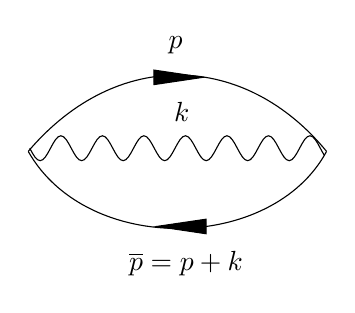
\begin{tikzpicture}[x=0.75pt,y=0.75pt,yscale=-1,xscale=1]
%uncomment if require: \path (0,300); %set diagram left start at 0, and has height of 300

%Curve Lines [id:da88424210762959] 
\draw    (391,142) .. controls (433.93,91.47) and (495.73,94.47) .. (534.73,142) ;
%Curve Lines [id:da08321555926143864] 
\draw    (391,142) .. controls (419.56,192.47) and (508.67,190.47) .. (534.73,142) ;
%Shape: Triangle [id:dp46422275430175963] 
\draw  [fill={rgb, 255:red, 0; green, 0; blue, 0 }  ,fill opacity=1 ] (475.23,106.3) -- (451.61,109.81) -- (451.51,102.81) -- cycle ;
%Shape: Triangle [id:dp600832008789588] 
\draw  [fill={rgb, 255:red, 0; green, 0; blue, 0 }  ,fill opacity=1 ] (453,178.15) -- (476.63,174.67) -- (476.7,181.67) -- cycle ;
%Shape: Wave [id:dp6468030283736343] 
\draw   (391.73,140.47) .. controls (393.36,143.54) and (394.92,146.47) .. (396.73,146.47) .. controls (398.54,146.47) and (400.1,143.54) .. (401.73,140.47) .. controls (403.36,137.39) and (404.92,134.47) .. (406.73,134.47) .. controls (408.54,134.47) and (410.1,137.39) .. (411.73,140.47) .. controls (413.36,143.54) and (414.92,146.47) .. (416.73,146.47) .. controls (418.54,146.47) and (420.1,143.54) .. (421.73,140.47) .. controls (423.36,137.39) and (424.92,134.47) .. (426.73,134.47) .. controls (428.54,134.47) and (430.1,137.39) .. (431.73,140.47) .. controls (433.36,143.54) and (434.92,146.47) .. (436.73,146.47) .. controls (438.54,146.47) and (440.1,143.54) .. (441.73,140.47) .. controls (443.36,137.39) and (444.92,134.47) .. (446.73,134.47) .. controls (448.54,134.47) and (450.1,137.39) .. (451.73,140.47) .. controls (453.36,143.54) and (454.92,146.47) .. (456.73,146.47) .. controls (458.54,146.47) and (460.1,143.54) .. (461.73,140.47) .. controls (463.36,137.39) and (464.92,134.47) .. (466.73,134.47) .. controls (468.54,134.47) and (470.1,137.39) .. (471.73,140.47) .. controls (473.36,143.54) and (474.92,146.47) .. (476.73,146.47) .. controls (478.54,146.47) and (480.1,143.54) .. (481.73,140.47) .. controls (483.36,137.39) and (484.92,134.47) .. (486.73,134.47) .. controls (488.54,134.47) and (490.1,137.39) .. (491.73,140.47) .. controls (493.36,143.54) and (494.92,146.47) .. (496.73,146.47) .. controls (498.54,146.47) and (500.1,143.54) .. (501.73,140.47) .. controls (503.36,137.39) and (504.92,134.47) .. (506.73,134.47) .. controls (508.54,134.47) and (510.1,137.39) .. (511.73,140.47) .. controls (513.36,143.54) and (514.92,146.47) .. (516.73,146.47) .. controls (518.54,146.47) and (520.1,143.54) .. (521.73,140.47) .. controls (523.36,137.39) and (524.92,134.47) .. (526.73,134.47) .. controls (528.54,134.47) and (530.1,137.39) .. (531.73,140.47) .. controls (532.4,141.73) and (533.06,142.97) .. (533.73,143.99) ;

% Text Node
\draw (467,196) node    {$\overline{p} =p+k$};
% Text Node
\draw (462,91) node    {$p$};
% Text Node
\draw (465,123) node    {$k$};


\end{tikzpicture}

    \caption{Vacuum Bubble Feynman Diagram}
    \label{fig:vacuum-bubble}
\end{figure}
\begin{qt}
    \begin{equation}
S_{F}^{(2)}=-\delta^{(4)}(0) \frac{e^{2}}{(2 \pi)^{4}} \iint S_{F \eta \alpha}(p+k) \gamma_{\alpha \beta}^{\mu} S_{F \beta \delta}(p) \gamma_{\delta \eta}^{\nu} i D_{F \mu \nu}(k) d^{4} k d^{4} p
\end{equation}
\end{qt}
In vacuum bubble means we start with zero 4-momentum in the vacuum, awe end with zero four-momentum in the vacuum, and in between we have a sum total 4 -momentum of zero for all the virtual particles mediating the interaction.

\section{Feynman Rules}
The rules themselves apply to what are termed \textbf{topologically different Feynman diagrams.} These are different from one another in ways other than simply changing labeling of vertices:
\begin{itemize}
    \item The S matrix element for a given interaction is 
    $$
S_{f i}=\delta_{f i}+\left((2 \pi)^{4} \delta^{(4)}\left(P_{f}-P_{i}\right)\right) (\prod^{\text {bosons }} \sqrt{\frac{1}{2 V \omega_{k}}})(\prod^{fermions} \sqrt{\frac{m}{V E_{\mathbf{P}}}})\mathcal{M}\quad\mathcal{M}=\sum_{n=1}^{\infty} \mathcal{M}^{(n)}
$$
where $P_{f}$ is the total 4-momentum of all final particles, $P_{i}$ is the total 4-momentum of all initial particles, and the contribution $\mathcal{M}^{(n)}$ comes from the $n$ th order perturbation term of the S operator, $S^{(n)}$
\item The Feynman amplitude $\mathcal{M}^{(n)}$ is obtained from all of the topologically distinct, connected (i.e., all lines connected to one another in a given diagram) Feynman diagrams which contain $n$ vertices. The contribution to each $\mathcal{M}^{(n)}$ is obtained by the following:

\begin{easylist}
  \ListProperties(Style1*=\bfseries,Numbers2=l,Mark1={},Mark2={)},Indent2=1em)
 @ For each vertex, include a factor $ie\gamma^{\mu}$
    
    @ For each internal photon line, labeled by 4-momentum $k$, include a factor $i D_{F \mu v}(k)=i \frac{-g_{\mu v}}{k^{2}+i \varepsilon}$
    
    @ For each internal fermion line, labeled by 4-momentum $p$, write a factor $i S_{F}(p)=i \frac{\not p+m}{p^{2}-m^{2}+i \varepsilon}$
    
    @ For each external line, write one of the following spinor factors, where $\mathbf{p}$ and $\mathbf{k}$ indicate basis states of corresponding 3 -momenta, $r$ represents spin state for fermions and polarization state for photons,
    @@ for each initial electron: $u_{r}(\mathbf{p})$
@@ for each final electron: $\bar{u}_{r}(\mathbf{p})$
@@ for each initial positron: $\bar{v}_{r}(\mathbf{p})$
@@ for each final positron: $v_{r}(\mathbf{p})$
@@ for each initial photon: $\varepsilon_{r, \mu}(\mathbf{k})$
@@ for each final photon: $\quad \varepsilon_{r, \mu}(\mathbf{k})$
@The spinor factors ( $\gamma$ matrices, $S_{F}$ functions, spinors) for each fermion line are ordered so that, reading from right to left, they occur in the same sequence as following the fermion line in the direction of its arrows through the vertex. (Order is important as it conveys spinor matrix multiplication order when we do not show spinor indices.)
@The four-momenta at each vertex are conserved (same total after as before).
@ For each closed loop of internal fermions only (without photons inside the loop itself, like what we call a "photon loop" which internally has an electron and a positron), take the trace (in spinor space) of the resulting matrix and multiply by a factor of $(-1)$
@ For each 4 -momentum $q$ which is not fixed by 4-momentum conservation, carry out the integration $\frac{1}{(2 \pi)^{4}} \int d^{4} q$ One such integration for each closed loop (fermion/fermion or fermion/photon loop).
@ Multiply the expression by (-1) for each interchange of neighboring fermion operators (each associated with a particular spinor factor) which would be required to place the expression in appropriate normal order. "Appropriate", when we are adding sub amplitudes, means each sub amplitude must be in the same, not just any, normal order of destruction and creation operators.
\end{easylist}
\end{itemize}
\begin{mybox}
Each term in $\mathcal{H}_I^I$, or equivalently in $\mathcal{L}_I^I$(since $\mathcal{L}_{I}^{I}=-\mathcal{H}_{I}^{I}$) results in a vertex interaction comprising the particles generated by the particular fields occurring in that term. Here so far, in QED, the only term in $\mathcal{L}_{I}^{I}$ is $\bar{\psi} \cancel{A} \psi$, so this gives rise to a vertex with two Dirac fermions and a photon.
\end{mybox}
\section{Including Other Charged Leptons in QED}
So far, we have dealt only with charged leptons of the electron/positron type. As physicists have learned from experiment, there are two more families of leptons, the muon/anti-muon (symbols
and $\mu^{\dagger}$ and the tau/anti-tau particle (symbols $\tau^{-}$ and $\tau^{+}$ ) families. Electrons, muons, and taus all have -1 charge. Positrons, anti-muons and anti-taus all have +1 charge. Electrons and positrons have the same mass. Muons and anti-muons have the same mass, which is about 200 times the electron mass. Taus and anti-taus have the same mass, which is about 170 times the muon mass. \textbf{The new interaction Hamiltonian that correctly describes all three families is}
\begin{equation}
\mathcal{H}_{I}^{I}=-\mathcal{L}_{I}^{I}=-e \sum_{l=1}^{3} \bar{\psi}_{l} A^{\mu} \gamma_{\mu} \psi_{l}=-e \sum_{l=1}^{3}\left(\bar{\psi}_{l}^{+}+\bar{\psi}_{l}^{-}\right)\left(\cancel{A}^{+}+\cancel{A}^{-}\right)\left(\psi_{l}^{+}+\psi_{l}^{-}\right)
\end{equation}
where the summation over $l$ represents a separate Hamiltonian density for electrons/positrons $(l=$
1), muons/anti-muons $(l=2),$ and taus/anti-taus $(l=3) .$ 
\subsection{Feynman Rules for Multiple Families}
\begin{easylist}
  @ Obtain the Feynman amplitude assuming all leptons are electrons/positrons
  @ For lines representing other lepton "flavors" replace spinor and/or propagators with those representing the other flavers.
  @ The only difference in the form of the result will be the masses.
\end{easylist}
\subsection{Elastic vs Inelastic Scattering}
The term inelastic scattering (or inelastic interaction) refers to \textbf{the particles involved changing into different types of particles with different masses (recall we mean "rest mass" by the term "mass")}, and hence some \bluep{kinetic energy must be converted into mass ( or vice versa depending on the particular interaction).}

The total amount of energy (in the form of mass plus kinetic energy) must stay the same. But if the total mass changes, then that change must be compensated for by an equivalent opposite change in kinetic energy.

Elastic scattering (or elastic interaction), on the other hand, implies we have the same type final particles (with the same masses) as the initial particles. No mass is created out of, or destroyed to yield, kinetic energy. \textbf{All energy exchange is purely kinetic, and this is a characteristic of classical elastic interactions, hence the name}.

\section{Attraction and Repulsion of Particles}
For virtual particles, \redp{3-momenturn can actually be in the opposite direction of velocity}. In fact, for attraction, this sort of behavior is essential. 3-momentum in other cases can be in other directions not parallel to virtual particle velocity (where we define that velocity in terms of the length vector between emission and absorption events divided by the time between them.)

Of course, in reality, we are looking at particles which are field-like in the sense that they are
spreading out in space. An interaction is more like an interaction of one particle field with another, and during this interaction, 3-momentum of.appropriate direction is transferred. Again, the Feynman diagrams tend to make us think of point-like particles, rather than field-like particles.

In all cases, however, we do find total 3-momentum and total energy, including all real and virtual particles, are conserved. These conservation laws still hold.

Now consider two macroscopic. charged objects approaching one another along the same line of action.When they are repulsing each other, they lose kinetic energy, and the total energy
$$
E_{\text {total}}=K E_{1}+V_{\text {classical}}+K E_{2}=\text { constant }
$$
where $V_{\text {classical}} \propto \frac{q_{1} q_{2}}{r}>0$. As their distance gets smaller, KE of the macro bodies decreases, but the electric field potential energy increases. In QFT, we would say the kinetic energies of the macro bodies plus all the energy of the virtuals is conserved,
$$
E_{\text {total}}=K E_{1}+E_{\text {virtuals}}+K E_{2}=\text { constant }
$$
And so, we can see that what is interpreted classically as classical field energy, is, in the quantum realm, energy of virtual particles,
$$
V_{\text {classical}}=E_{\text {virtuals}}>0
$$

Similar to repulsion, the classical energy relation for attraction is
$$
E_{\text {total}}=K E_{1}+V_{\text {cluascical}}+K E_{2}=const.
$$
where $V_{\text {classical}} \propto \frac{q_{1} q_{2}}{r}<0$. Given that we must have the same energy relation, in terms of virtual particles, it must mean that \textbf{the virtual particles energy must be negative as two objects approach}.
% Please add the following required packages to your document preamble:
% 
\begin{table}[H]
\caption{Summary of Virtual Photon Properties for 1D Attraction and Repulsion}
\centering
\begin{tabular}{|c|c|c|c|c|}
\hline
\multirow{2}{*}{}                                                          & \multicolumn{2}{c|}{Virtual particles in repulsion} & \multicolumn{2}{c|}{virtual particle in attraction} \\ \cline{2-5} 
                                                                           & 3-momentum                      & Energy            & 3-momentum                       & Energy           \\ \hline
\begin{tabular}[c]{@{}c@{}}Approaching and receding\\ objects\end{tabular} & $\mathbf{v}$ direction          & positive          & $-\mathbf{v}$ direction          & negative         \\ \hline
\end{tabular}
\end{table}

\section{A Solved Exercise}
Draw the two Feynman diagram for the interaction $\gamma \gamma \rightarrow e^{+} e^{-} .$ Using Feynman's rules, write out the amplitude for one of the diagrams.

\textbf{Solution}

\begin{figure}[H]
    \centering
\tikzset{every picture/.style={line width=0.75pt}} %set default line width to 0.75pt        

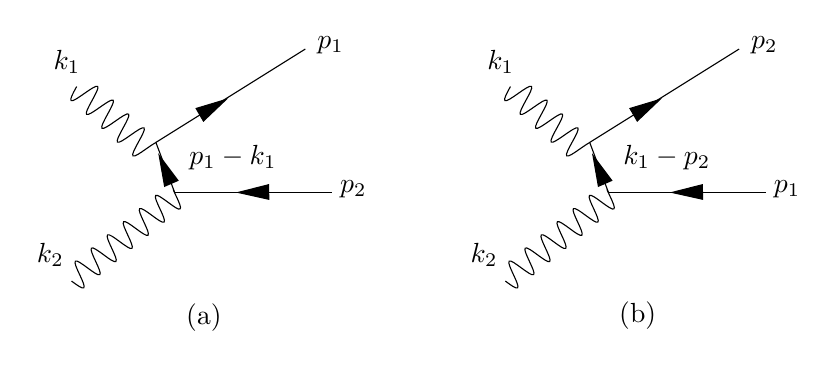
\begin{tikzpicture}[x=0.75pt,y=0.75pt,yscale=-1,xscale=1]
%uncomment if require: \path (0,300); %set diagram left start at 0, and has height of 300

%Shape: Wave [id:dp42261345767317293] 
\draw   (79.69,79.75) .. controls (77.97,82.9) and (76.33,85.9) .. (77,86.5) .. controls (77.68,87.1) and (80.48,85.14) .. (83.41,83.09) .. controls (86.35,81.03) and (89.15,79.07) .. (89.82,79.67) .. controls (90.5,80.28) and (88.86,83.27) .. (87.14,86.42) .. controls (85.42,89.57) and (83.78,92.56) .. (84.46,93.17) .. controls (85.13,93.77) and (87.93,91.81) .. (90.87,89.75) .. controls (93.8,87.7) and (96.6,85.74) .. (97.28,86.34) .. controls (97.95,86.94) and (96.31,89.94) .. (94.59,93.09) .. controls (92.87,96.24) and (91.23,99.23) .. (91.91,99.84) .. controls (92.58,100.44) and (95.38,98.48) .. (98.32,96.42) .. controls (101.25,94.36) and (104.05,92.41) .. (104.73,93.01) .. controls (105.4,93.61) and (103.76,96.61) .. (102.04,99.76) .. controls (100.32,102.9) and (98.68,105.9) .. (99.36,106.51) .. controls (100.03,107.11) and (102.83,105.15) .. (105.77,103.09) .. controls (108.7,101.03) and (111.5,99.08) .. (112.18,99.68) .. controls (112.85,100.28) and (111.22,103.28) .. (109.49,106.43) .. controls (107.77,109.57) and (106.13,112.57) .. (106.81,113.18) .. controls (107.48,113.78) and (110.28,111.82) .. (113.22,109.76) .. controls (115,108.52) and (116.72,107.31) .. (117.96,106.68) ;
%Shape: Wave [id:dp4663385617467217] 
\draw   (77.23,173.48) .. controls (79.89,175.43) and (82.42,177.29) .. (83.12,176.72) .. controls (83.82,176.15) and (82.5,173.3) .. (81.1,170.31) .. controls (79.71,167.32) and (78.39,164.48) .. (79.09,163.9) .. controls (79.79,163.33) and (82.32,165.19) .. (84.97,167.15) .. controls (87.63,169.1) and (90.16,170.96) .. (90.86,170.39) .. controls (91.56,169.81) and (90.23,166.97) .. (88.84,163.98) .. controls (87.45,160.99) and (86.13,158.14) .. (86.83,157.57) .. controls (87.53,157) and (90.06,158.86) .. (92.71,160.81) .. controls (95.37,162.77) and (97.89,164.63) .. (98.6,164.05) .. controls (99.3,163.48) and (97.97,160.63) .. (96.58,157.64) .. controls (95.19,154.66) and (93.87,151.81) .. (94.57,151.24) .. controls (95.27,150.66) and (97.8,152.52) .. (100.45,154.48) .. controls (103.1,156.43) and (105.63,158.29) .. (106.33,157.72) .. controls (107.03,157.15) and (105.71,154.3) .. (104.32,151.31) .. controls (102.93,148.32) and (101.6,145.48) .. (102.3,144.9) .. controls (103,144.33) and (105.53,146.19) .. (108.19,148.14) .. controls (110.84,150.1) and (113.37,151.96) .. (114.07,151.39) .. controls (114.77,150.81) and (113.45,147.97) .. (112.06,144.98) .. controls (110.66,141.99) and (109.34,139.14) .. (110.04,138.57) .. controls (110.74,138) and (113.27,139.85) .. (115.93,141.81) .. controls (118.58,143.77) and (121.11,145.62) .. (121.81,145.05) .. controls (122.51,144.48) and (121.19,141.63) .. (119.8,138.64) .. controls (118.4,135.65) and (117.08,132.81) .. (117.78,132.23) .. controls (118.48,131.66) and (121.01,133.52) .. (123.66,135.48) .. controls (126.32,137.43) and (128.85,139.29) .. (129.55,138.72) .. controls (130.25,138.14) and (128.93,135.3) .. (127.53,132.31) .. controls (127.05,131.28) and (126.58,130.26) .. (126.19,129.35) ;
%Straight Lines [id:da1794479383390909] 
\draw    (126.87,130.67) -- (202.87,130.67) ;
%Straight Lines [id:da4474428063722128] 
\draw    (126.87,130.67) -- (117.87,106.67) ;
%Straight Lines [id:da25489428858325125] 
\draw    (117.87,106.67) -- (189.87,61.67) ;
%Shape: Triangle [id:dp9417697592251211] 
\draw  [fill={rgb, 255:red, 0; green, 0; blue, 0 }  ,fill opacity=1 ] (157.53,130.78) -- (172.15,127.06) -- (172.25,134.05) -- cycle ;
%Shape: Triangle [id:dp905894856195697] 
\draw  [fill={rgb, 255:red, 0; green, 0; blue, 0 }  ,fill opacity=1 ] (119.45,112.94) -- (128.49,125) -- (122.07,127.79) -- cycle ;
%Shape: Triangle [id:dp730772445251452] 
\draw  [fill={rgb, 255:red, 0; green, 0; blue, 0 }  ,fill opacity=1 ] (151.71,85.98) -- (140.78,96.38) -- (137.27,90.32) -- cycle ;
%Shape: Wave [id:dp5681697616106831] 
\draw   (288.69,79.75) .. controls (286.97,82.9) and (285.33,85.9) .. (286,86.5) .. controls (286.68,87.1) and (289.48,85.14) .. (292.41,83.09) .. controls (295.35,81.03) and (298.15,79.07) .. (298.82,79.67) .. controls (299.5,80.28) and (297.86,83.27) .. (296.14,86.42) .. controls (294.42,89.57) and (292.78,92.56) .. (293.46,93.17) .. controls (294.13,93.77) and (296.93,91.81) .. (299.87,89.75) .. controls (302.8,87.7) and (305.6,85.74) .. (306.28,86.34) .. controls (306.95,86.94) and (305.31,89.94) .. (303.59,93.09) .. controls (301.87,96.24) and (300.23,99.23) .. (300.91,99.84) .. controls (301.58,100.44) and (304.38,98.48) .. (307.32,96.42) .. controls (310.25,94.36) and (313.05,92.41) .. (313.73,93.01) .. controls (314.4,93.61) and (312.76,96.61) .. (311.04,99.76) .. controls (309.32,102.9) and (307.68,105.9) .. (308.36,106.51) .. controls (309.03,107.11) and (311.83,105.15) .. (314.77,103.09) .. controls (317.7,101.03) and (320.5,99.08) .. (321.18,99.68) .. controls (321.85,100.28) and (320.22,103.28) .. (318.49,106.43) .. controls (316.77,109.57) and (315.13,112.57) .. (315.81,113.18) .. controls (316.48,113.78) and (319.28,111.82) .. (322.22,109.76) .. controls (324,108.52) and (325.72,107.31) .. (326.96,106.68) ;
%Shape: Wave [id:dp9172238171778244] 
\draw   (286.23,173.48) .. controls (288.89,175.43) and (291.42,177.29) .. (292.12,176.72) .. controls (292.82,176.15) and (291.5,173.3) .. (290.1,170.31) .. controls (288.71,167.32) and (287.39,164.48) .. (288.09,163.9) .. controls (288.79,163.33) and (291.32,165.19) .. (293.97,167.15) .. controls (296.63,169.1) and (299.16,170.96) .. (299.86,170.39) .. controls (300.56,169.81) and (299.23,166.97) .. (297.84,163.98) .. controls (296.45,160.99) and (295.13,158.14) .. (295.83,157.57) .. controls (296.53,157) and (299.06,158.86) .. (301.71,160.81) .. controls (304.37,162.77) and (306.89,164.63) .. (307.6,164.05) .. controls (308.3,163.48) and (306.97,160.63) .. (305.58,157.64) .. controls (304.19,154.66) and (302.87,151.81) .. (303.57,151.24) .. controls (304.27,150.66) and (306.8,152.52) .. (309.45,154.48) .. controls (312.1,156.43) and (314.63,158.29) .. (315.33,157.72) .. controls (316.03,157.15) and (314.71,154.3) .. (313.32,151.31) .. controls (311.93,148.32) and (310.6,145.48) .. (311.3,144.9) .. controls (312,144.33) and (314.53,146.19) .. (317.19,148.14) .. controls (319.84,150.1) and (322.37,151.96) .. (323.07,151.39) .. controls (323.77,150.81) and (322.45,147.97) .. (321.06,144.98) .. controls (319.66,141.99) and (318.34,139.14) .. (319.04,138.57) .. controls (319.74,138) and (322.27,139.85) .. (324.93,141.81) .. controls (327.58,143.77) and (330.11,145.62) .. (330.81,145.05) .. controls (331.51,144.48) and (330.19,141.63) .. (328.8,138.64) .. controls (327.4,135.65) and (326.08,132.81) .. (326.78,132.23) .. controls (327.48,131.66) and (330.01,133.52) .. (332.66,135.48) .. controls (335.32,137.43) and (337.85,139.29) .. (338.55,138.72) .. controls (339.25,138.14) and (337.93,135.3) .. (336.53,132.31) .. controls (336.05,131.28) and (335.58,130.26) .. (335.19,129.35) ;
%Straight Lines [id:da804466301192061] 
\draw    (335.87,130.67) -- (411.87,130.67) ;
%Straight Lines [id:da9456286266176618] 
\draw    (335.87,130.67) -- (326.87,106.67) ;
%Straight Lines [id:da029609280510542235] 
\draw    (326.87,106.67) -- (398.87,61.67) ;
%Shape: Triangle [id:dp22104050771755757] 
\draw  [fill={rgb, 255:red, 0; green, 0; blue, 0 }  ,fill opacity=1 ] (366.53,130.78) -- (381.15,127.06) -- (381.25,134.05) -- cycle ;
%Shape: Triangle [id:dp9760192036699857] 
\draw  [fill={rgb, 255:red, 0; green, 0; blue, 0 }  ,fill opacity=1 ] (328.45,112.94) -- (337.49,125) -- (331.07,127.79) -- cycle ;
%Shape: Triangle [id:dp5166985545513405] 
\draw  [fill={rgb, 255:red, 0; green, 0; blue, 0 }  ,fill opacity=1 ] (360.71,85.98) -- (349.78,96.38) -- (346.27,90.32) -- cycle ;

% Text Node
\draw (202,60) node    {$p_{1}$};
% Text Node
\draw (213,129) node    {$p_{2}$};
% Text Node
\draw (155,114) node    {$p_{1} -k_{1}$};
% Text Node
\draw (75,68) node    {$k_{1}$};
% Text Node
\draw (67,161) node    {$k_{2}$};
% Text Node
\draw (411,60) node    {$p_{2}$};
% Text Node
\draw (422,129) node    {$p_{1}$};
% Text Node
\draw (364,114) node    {$k_{1} -p_{2}$};
% Text Node
\draw (284,68) node    {$k_{1}$};
% Text Node
\draw (276,161) node    {$k_{2}$};
% Text Node
\draw (141,191) node   [align=left] {(a)};
% Text Node
\draw (350,190) node   [align=left] {(b)};


\end{tikzpicture}

    \caption{Feynman's diagram for $\gamma \gamma \rightarrow e^{+} e^{-}$}
    \label{fig:rree-diagram}
\end{figure}
\bluep{Note the positron propagator relations will carry 4-momentum with opposite sign of what we would find physically,i.e., $k_1=p_1+\bar{q}_{phys}\rightarrow\bar{q}_{phys}=k_1-p_1\rightarrow\bar{q}=p_1-k_1$ in going from left to right time flow.}

Follow direction of fermion arrows thru RH vertex: $iS_F(p_1-k_1)ie\gamma^{\nu}v_{r_2}(\mathbf{p}_2)$

Including other vertex (LH one) fermion only: $\bar{u}_{r_1}(\mathbf{p}_1)ie\gamma^{\mu}iS_F(p_1-k_1)ie\gamma^{\nu}v_{r_2}(\mathbf{p}_2)$

Including external initial photons: $\bar{u}_{r_1}(\mathbf{p}_1)ie\gamma^{\mu}iS_F(p_1-k_1)ie\gamma^{\nu}v_{r_2}(\mathbf{p}_2)\varepsilon_{\mu,r_1}(\mathbf{k}_1)\varepsilon_{\nu,r_3}(\mathbf{k}_2)$

Thus, $\mathcal{M}^{(2)}_{(a)}=-e^2\bar{u}_{r_1}(\mathbf{p}_1)\gamma^{\mu}iS_F(p_1-k_1)\gamma^{\nu}v_{r_2}(\mathbf{p}_2)\varepsilon_{\mu,r_1}(\mathbf{k}_1)\varepsilon_{\nu,r_3}(\mathbf{k}_2)$, where
$$
S^{(2)}_{\gamma \gamma \rightarrow e^{+} e^{-}}=\frac{1}{2V\sqrt{\omega_1\omega_2}}\frac{m}{2V\sqrt{E_1E_2}}(2\pi)^4\delta^{(4)}(p_1+p_2-k_1-k_2)(\mathcal{M}^{(2)}_{(a)}+\mathcal{M}^{(2)}_{(b)})
$$
\end{document}
